% !TEX TS-program = pdflatex
% !TEX encoding = UTF-8 Unicode

%\documentclass[a4paper,twoside]{article}%                                        use larger type; default would be 10pt
\documentclass[a4paper]{article}%                                                 use larger type; default would be 10pt
\usepackage[utf8]{inputenc}%                                                      set input encoding (not needed with XeLaTeX)

%%% PAGE DIMENSIONS ------------------------------------------------------------
\usepackage{geometry}%              to change the page dimensions
\geometry{a4paper}%                                                               or letterpaper (US) or a5paper or....
\usepackage[parfill]{parskip}%                                                    Activate to begin paragraphs with an empty line rather than an indent

%%% HEADERS & FOOTERS ----------------------------------------------------------
\usepackage{fancyhdr}%                                                            This should be set AFTER setting up the page geometry
\pagestyle{fancy}%                                                                options: empty , plain , fancy
\renewcommand{\headrulewidth}{0pt}%                                               customise the layout...
\lhead{}\chead{}\rhead{}
\lfoot{}\cfoot{page \thepage}\rfoot{}

%%% SECTION TITLE APPEARANCE ---------------------------------------------------
\usepackage{sectsty}
\allsectionsfont{\sffamily\mdseries\upshape}%                                     (See the fntguide.pdf for font help)

%%% PACKAGES -------------------------------------------------------------------
\usepackage[font=small,labelfont=bf,textfont=it]{caption}%                        stylize captions
\usepackage[pdftex]{graphicx}%                                                    support the \includegraphics command and options
\usepackage{booktabs}%                                                            for much better looking tables
\usepackage{array}%                                                               for better arrays (eg matrices) in maths
\usepackage{paralist}%                                                            very flexible & customisable lists (eg. enumerate/itemize, etc.)
\usepackage{verbatim}%                                                            adds environment for commenting out blocks of text & for better verbatim
\usepackage{subfig}%                                                              make it possible to include more than one captioned figure/table in a single float
\usepackage{mathtools}%                                                           for math environments like align
\usepackage{amssymb}%                                                             for symbols like \therefore
\usepackage{verbatim}%                                                            for including text as appears, verbatim
\usepackage{listings}%                                                            for including external files as text, eg code
\usepackage{color}%                                                               for coloring of files and images
\usepackage{overpic}%                                                             for adding annotations to pictures
\usepackage[alsoload=astro]{siunitx}%                                                             for units \SI{}{}, \si{}, \num{} etc.
\usepackage{multirow}%                                                            for multiple row spanning cells in tables
\usepackage{rotating}%                                                            for the \begin{sideways} environment for sideways text

%%% EQUATIONS ------------------------------------------------------------------
\numberwithin{equation}{section}%                                                 Number equations by section (change for different levels)
	\DeclareSIUnit\pixel{pix}
	\DeclareSIUnit\ADU{ADU}
    \DeclareSIUnit\electron{\text{e}^{-{}}}
	\DeclareSIUnit\erg{erg}
    \DeclareSIUnit\year{yr}

%% BIBIOGRAPHY ------------------------------------------------------------------
\usepackage{cite}

%%% ToC (table of contents) APPEARANCE -----------------------------------------
%\usepackage[nottoc,notlof,notlot]{tocbibind}                                   % Put the bibliography in the ToC
%\usepackage[titles,subfigure]{tocloft}                                         % Alter the style of the Table of Contents
%\renewcommand{\cftsecfont}{\rmfamily\mdseries\upshape}
%\renewcommand{\cftsecpagefont}{\rmfamily\mdseries\upshape}                     % No bold!
\setcounter{tocdepth}{2}

%%% PDF LINKS AND STYLE --------------------------------------------------------
\usepackage[unicode=true,
    bookmarks=true,bookmarksnumbered=true,bookmarksopen=true,
    bookmarksopenlevel=2, breaklinks=false,pdfborder={0 0 0},backref=false,
    colorlinks=false] {hyperref}%                                                 for links in pdf file, no colors
\hypersetup{pdftitle={Cosmic Re-ionisation},
    pdfauthor={Extragalactic Astrophysics and Cosmology Group Studies}}%		  set name of document and author here

%%% END Article customizations

%%% NEW COMMANDS ---------------------------------------------------------------
\renewcommand{\d}{\,\mathrm{d}}%                                                  for integrals
\newcommand{\dx}[2]{\frac{\textrm{d}#1}{\textrm{d}#2}}%                           for derivatives
\newcommand{\dd}[2]{\frac{\textrm{d}^2#1}{\textrm{d}#2^2}}%                       for double derivatives
\newcommand{\pd}[2]{\frac{\partial#1}{\partial#2}}%                               for partial derivatives
\newcommand{\pdd}[2]{\frac{\partial^2#1}{\partial#2^2}}%                          for double partial derivatives
\newcommand{\e}[1]{\text{e}^{#1}}%                                                for exponentials
\newcommand{\code}[1]{\texttt{#1}}%                                               for verbatim code view
\newcommand{\inter}[1]{\shortintertext{#1}}%                                      shorter version of intertext
\newcommand{\under}[1]{\underline{#1}}%                                           for vectors etc.

\let\vaccent=\v{}%                                                                rename builtin command \v{} to \vaccent{}
\newcommand{\uv}[1]{\ensuremath{\hat{#1}}}%                                       for unit vector
\newcommand{\abs}[1]{\left|#1\right|}%                                            for absolute value
\newcommand{\avg}[1]{\left<#1\right>}%                                            for average
\let\underdot=\d%                                                                 rename builtin command \d{} to \underdot{}
\newcommand{\ket}[1]{\left|#1\right>}%                                            for Dirac bras
\newcommand{\bra}[1]{\left<#1\right|}%                                            for Dirac kets
\newcommand{\braket}[2]{\left<#1\vphantom{#2} \right|
    \left.#2 \vphantom{#1} \right>}%                                              for Dirac brackets
\newcommand{\matrixel}[3]{\left<#1\vphantom{#2#3} \right|
    #2 \left|#3 \vphantom{#1#2}\right>}%                                          for Dirac matrix elements
\newcommand{\grad}[1]{\nabla#1}%                                                  for gradient
\let\divsymb=\div%                                                                rename builtin command \div to \divsymb
\renewcommand{\div}[1]{\nabla\cdot#1}%                                            for divergence
\newcommand{\curl}[1]{\nabla\times#1}%                                            for curl
\let\baraccent=\={}%                                                              rename builtin command \= to \baraccent
\renewcommand{\=}[1]{\stackrel{#1}{=}}%                                           for putting numbers above =

\newcolumntype{L}{>{\centering\arraybackslash}m{3em}}

%*******************************************************************************
%******************************** END HEADER ***********************************
%*******************************************************************************

\begin{document}
%!TEX root = mainfile.tex
\begin{titlepage}
  \begin{center}
    \vspace*{\fill}

    \centering
    
\includegraphics[scale=1.0]{Logo.pdf}
    \vfill

    \hrule
    {\LARGE\bf Extragalactic Astrophysics and Cosmology\\Cosmic Reionization \\[0.4cm]}
    \hrule

    \vfill
    \large
    School of Physics and Astronomy\\
    University of Birmingham

    \vfill
    { Joe Baumber,
    	James Bryant,
    	Lewis Clegg,
    	Bethany Johnson,
    	Andrew King,
    	Owen McConnell,
    	Catherine McDonald,
    	Michael O'Neill,
    	Jonathan Shepley,
    	Dorothy Stonell,
    	Rahim Topadar,
    	Josh Wainwright\\}
    \vfill

    \vfill
    \textit{Supervisors:} Graham Smith, Alistair Sanderson, Melissa Gillone \\
    		\vfill
    \textit{Date:} March 2013
    \vfill
    \vfill

    \begin{abstract}
        This study deduces that reionization began at a redshift of $z=17.82$ and ended at a redshift of $z=7\pm 1.8$. This is calculated by directly applying the dynamics of star formation and the ionization rate of neutral hydrogen in the Intergalactic Medium. A photometry strategy consisting of 3 multi-band surveys is proposed in order to observe Lyman Break Galaxies across redshifts 6--17. The surveys will locate $100.5\pm37.0$, $138.7\pm 100.6$, $358.1\pm 158.6$ galaxies in redshift ranges 6--8.5, 8.5--10 and 10--17 respectively. These surveys will be completed by the James Webb Space Telescope and Euclid which are planned for launch in the coming decade. A follow up spectroscopy survey will be used to confirm the redshift and properties of 24, 4 and 48 galaxies in these 3 surveys respectively. The spectroscopy will be carried out using James Webb Space Telescope and a combination of single and multi-slit spectroscopy. It is shown that the use of known gravitational lenses, located between redshift 0.5--0.7, is very beneficial for discovering high redshift candidates as it can increase the depth of surveys by up to 3 magnitudes.
    \end{abstract}


  \end{center}
\end{titlepage}

%\thispagestyle{empty}
%\vspace*{\fill}
%\noindent
%\begin{tabular}{ll}
%\end{tabular}

%\cleardoublepage
%\cleardoublepage

\newpage
\tableofcontents
\addcontentsline{toc}{section}{Contents}
\listoffigures
\listoftables
\newpage

\pagestyle{headings}
    %!TEX root = mainfile.tex

\section{Introduction} %fold
\label{section:Introduction}
	The evolution of the Universe has been divided up by cosmologists into several epochs; each characterised by their unique physical properties. This project focuses on the Epoch of Re-ionization (EoR) whereby high energy photons produced during active star formation ionized the neutral hydrogen in the Inter-Galactic Medium (IGM). In order to probe this particular era and learn more about it, early (high redshift) galaxies are being studied as it is believed that they produced these first ionizing photons and hence their birth should understandably correlate directly to the beginning of the Epoch of Cosmic Re-ionization. (more detail in section~\ref{sec:cosmic_re_ionisation}).

	There are many unanswered questions in cosmology; one of the most crucial is the nature of dark energy and matter which make up around 95\% of the universe\cite{WMAP9}. These mysterious substances are thought to be the key driving force behind the evolution and expansion of the universe. By studying and mapping the distribution of Hydrogen during the EoR and tracking the evolution of stars and galaxies we are able to infer more about the effects of dark energy and what it might consist of. There are many different theories about what dark matter consist of; the current most popular theories fall under the ``Cold Dark Matter'' model where dwarf galaxies are thought to be key building blocks in the hierarchical structure formation of the first galaxies\cite{Cignoni}.

	The process of Cosmic Re-ionization is crucial to our understanding of the evolution of the Universe as it forms the bridge between our present and a distant, ill-understood past. It links our current familiar universe whereby stars and galaxies are more common than the grains of sand on Earth's beaches to its past; when the Universe was a barren soup of free particles devoid of structure and life as we know it. Understanding the mechanisms of structure formation and what drives the collapse and formation of structure is fundamental in refining the Concordance Cosmology Model. Completing the picture of what happened during the EoR will enable us to more accurately predict where the Universe is headed and how it may eventually end, will it be in a ``big crunch'' or a ``big freeze''?

	The light from this era is so far away, and hence dim, that technology is only just allowing astronomers to see these early galaxies using high-powered telescopes and sophisticated detection process. There are a number of different projects in progress investigating this particular period of the universe and there are many more in the pipeline, these will be discussed in more detail in part~\ref{prt:observations}.

    \subsection{Structure of Study} %fold
    \label{Structure_of_Study}
		This study aims to develop an observing strategy based on original calculations for galaxy distributions and ultimately estimate the redshift range over which the EoR occurred. The group is split into two subgroups; a predictions group and an observational strategy group. The principal aim of the predictions group is to produce a set of calculations yielding the number of galaxies within the appropriate range of redshifts for re-ionization, with the inclusion of influences such as cosmic variance which skew the distribution. By considering the star formation rates and the ionization rate of neutral hydrogen the upper and lower bounds of this range respectively is determined. The final observing strategy explores which facilities to use; both current and planned and any adjustments required. The plan calculates the amount of observing time required to identify and confirm the properties of galaxies during the EoR. It also considers how to limit objects which will spoil our results; contaminants such as foreground stars and Supernovae events. The strategy aims to see further than previously achieved in this field and help to drive the understanding of re-ionization to new heights.
	%subsection Structure_of_Study (end)
%section Introduction (end)

\newpage

\part{General Theory} % (fold)
\label{prt:general_theory}
    %!TEX root = mainfile.tex

\section{Cosmic Re-Ionization} % (fold)
\label{sec:cosmic_re_ionisation}
	It is now universally accepted that the Universe began with the Big Bang whereby matter erupted from a singularity in an unexplained burst of energy. Following this the Universe was so hot (approximately $10^{12}$--$10^{15}$\,\si{\kelvin}\cite{liddle2003introduction}) that the photons had enough energy to suppress the binding of nucleons and so the Universe remained a soup of free baryons, leptons and energetic photons (amongst other things) until just a few minutes after the Big Bang during the Epoch of Nucleosynthesis when the protons and neutrons could begin to form atomic nuclei. Approximately \num{300000} years after the Big Bang came the Epoch of Decoupling when the majority of photons had lost a large proportion of their energy from frequent collisions within the plasma and hence most were left with less than the minimum hydrogen ionization energy of \SI{13.6}{\electronvolt}\cite{liddle2003introduction}. This allowed the electrons to finally bind to the hydrogen nuclei to form neutral hydrogen atoms, free from interfering photons. These newly retired photons were now able to travel across the Universe. With the photons having too little energy to interact with matter the Universe had become a transparent highway to our present and the photons set out on a journey which lasted almost as long as the age of the Universe, eventually arriving at Earth as a blanket of radiation known as the Cosmic Microwave Background.

	Meanwhile, in the wake of Decoupling matter was able to interact without disturbance from photons; atomically and gravitationally. Small density fluctuations, seen from Earth as small temperature fluctuations in the Cosmic Microwave Background, began to grow to such an extent that their gravity became large enough to attract matter, as more and more matter was attracted the gravitation became stronger and hence attracted more matter. This was the beginning of structure formation and the era known as ``Cosmic Re-ionization''. As more and more matter accumulated, stars began to form with high enough core temperatures to create photons with enough energy to once again ionize the neutral hydrogen in the IGM. As more stars formed, more of these high energy photons were being produced; gradually transforming the dark, neutral Universe to its current ionized state.

	In order for these photons to ionize the IGM, they evidently must reach it and hence must escape from their resident galaxy. The rate at which these photons were produced and escaped determines the length of time over which re-ionization occurred if one defines the end of re-ionization as being the point at which all, or at least the vast majority, of neutral hydrogen has been ionized. This requires one to understand how these early galaxies formed and thus infer their characteristic temperatures to see how many photons may have had enough energy to fully ionize the neutral hydrogen. Then one must consider what fraction of these photons could escape from the galaxy having managed to avoid interactions with the dust and neutral hydrogen within it. The specifics of this topic will be covered in more detail in Section~\ref{sec:determining_the_rate_of_re_ionizing_photons}.
% section cosmic_re_ionisation (end)

    %!TEX root = mainfile.tex

\section{Gravitational Lensing} % (fold)
\label{sec:gravitational_lensing}

	\subsection{Introduction} % (fold)
	\label{sub:introduction}
		Contrary to a popularly held belief that it was Newton who first referred to gravitational lensing in his publication ``Opticks''\cite{Newton_Opticks} (put into context, it is clear that he was discussing diffraction), the first person to allude directly to the bending of light due to gravitational attraction was Henry Cavendish. Around the turn of the 19th century Cavendish used Newton's corpuscular theory to correctly calculate the bending of light around a massive object.  Around the same time, German astronomer Johann Soldner was independently addressing the same problem\cite{Soldner} and although his results were similar to those obtained by Cavendish, his method was fundamentally flawed due to incorrect assumptions\cite{Conceptual_origins_of_GL}.

		The subject of gravitational lensing was then largely put to rest until 1915 when Einstein postulated his theory of General Relativity, from which it is clear that massive objects will cause light to bend as a result of the curvature of spacetime. Despite having complete and correct calculations of the phenomenon of gravitational lensing, including the lens equation and the position of images, Einstein displayed very little interest in it. He mentions it only briefly in his notebooks and published a single, very short discussion in Science Magazine upon the request of a friend at the end of which he dismissively comments that there is ``no great chance of this phenomenon being observed''\cite{Einstein_science_magazine}.

		During a solar eclipse in 1919, Eddington measured the positions of stars lying close to the Sun and observed that their positions appeared at a greater distance from the Sun than expected, thereby giving the first experimental evidence for the bending of light around the Sun\cite{Eddington_GL_evidence}. 5 years later, Chwolson published a paper on the idea that `fake double stars' may be observed as a result of the gravitational lensing effect and postulated that if source, lens and observer are perfectly aligned then a `Chwolson ring', later renamed ``Einstein ring'', would form around the lens\cite{Conceptual_origins_of_GL}.

		The true pioneer of the subject, however, is generally considered to be Czech astronomer\cite{F_Link_GL} Frantisek Link. Through detailed calculations of image magnification and positions, Link concluded that in some cases gravitational lensing would make faint sources visible. Optimistic about the possibility of observing these sources, particularly for spiral nebulae, he published a detailed paper on his wide ranging calculations which included the deflection undergone by light rays passing massive objects, the resulting change in intensity of sources and the invariance of source surface brightness. Following this, there was again a period of lack of interest, during which only a few papers were published on the subject until the discovery of the first lens in 1979 by Walsh, Carswell and Weymann. From here onwards, it became a topic of intense interest to astronomers and many more lenses and faint sources have since been discovered\cite{Conceptual_origins_of_GL}.
	% subsection introduction (end)

	\subsection{Concept} % (fold)
	\label{sub:concept}
		The bending of light around a massive object is a direct result of Einstein's theory of relativity and the curvature of spacetime. This effect can cause massive objects to act as lenses for background sources by bending the light such that rays that otherwise would not have been detected converge at the observer, resulting in a brighter image being observed. The increase in flux reaching the observer can result in significant magnification of a source, for example, one of the most distant objects known was observed behind the cluster Abell 2218 with a magnification factor of 30, equivalent to a decrease of 3.7 AB magnitudes\cite{Distant_object_Abell2218}. Studying the magnification and properties of the images can yield information about both the lens and the source, making it an extremely useful tool\cite{Hartle}.
		\begin{figure}[!htbp]
			\centering
				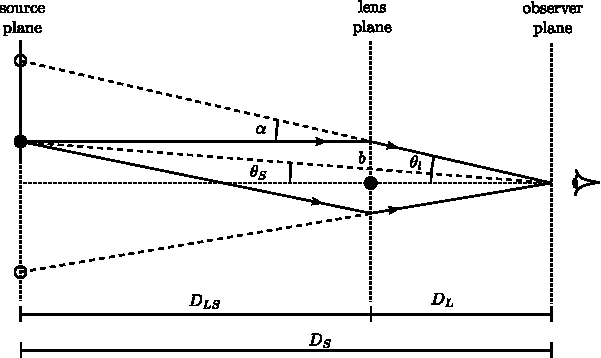
\includegraphics[width=0.6\textwidth]{../Images/Lensing_light_bending.pdf}
			\caption[Diagram of a gravitational lens]{In this schematic diagram of a gravitational lens, DL, DS and DLS represent the observer-lens, observer-source and lens-source distances respectively. $\theta_i$ is the image angle and $\theta_S$ the source angle, relative to the observer-lens axis. The light ray (solid line) passes by the lens at impact parameter $b$ and as a result is deflected by angle $\alpha$, converging with a second ray at the observer. The dotted lines indicate the position at which the images are observed\cite{Lensing_light_bending_diagram}.\label{fig:Lensing_light_bending}}
		\end{figure}

		The schematic diagram in Figure~\ref{fig:Lensing_light_bending} shows a gravitational lens acting on light from a background source in such a way as to form two images. The distances between observer, lens and source are so large in comparison to the impact parameter $b$ that to good approximation, the lens radius is negligible and it can be modelled as a thin lens. It is therefore reasonable to assume that the light travels in straight lines at all times except in the lens plane where the complete deflection occurs. Furthermore, it can be assumed that for all values of $b$, the deflection angle is given by
		\begin{align}
			\alpha &= \frac{4GM}{c^2 b}
		\end{align}
		where $M$ is the mass of the lens, c the speed of light and $G$ is the gravitational constant. In realistic lensing situations, all the angles shown in Figure~\ref{fig:Lensing_light_bending} are very small, hence the small angle approximation can be applied to yield the lens equation
		\begin{align}
			\theta_i D_S &= \theta_S D_S + \alpha D_{LS}
		\end{align}
		and also to approximate the impact parameter to $b\approx\theta_i DL$, it follows that
		\begin{align}
			\theta_i &= \theta_S + \frac{\theta_E^2}{\theta_i} \label{eq:einstein_angle}
		\end{align}
		where $\theta_E$ corresponds to the Einstein angle (or Einstein radius), given by
		\begin{align}
			\theta_E &= \frac{4GM}{c^2}\frac{D_{LS}}{D_L D_S}
		\end{align}
		sets the characteristic angular scale for any lensing system\cite{Hartle}.

		Lensing in which multiple images are formed and the source is significantly magnified is known as strong lensing. For strong lensing to occur, it is a mathematical requirement for the projected surface density to be greater than the critical surface density which is given by\cite{Critical_surface_density}
		\begin{align}
			\Sigma_c &= \frac{c^2}{4\pi G}\frac{D_S}{D_L D_{LS}}
		\end{align}
		Usually strong lensing requires the lens to have a high mass and the source angle $\theta_S$ to be relatively small. In the rare case that the source, lens and observer in a lensing system are perfectly aligned, a ring of light is observed around the lens, known as an Einstein ring. This ring will be at a constant distance from the centre of the ring equal to the Einstein radius. More commonly, the source is offset from the observer-lens axis, resulting in the formation of multiple images. The number of images formed by a lens is always odd, however, using the limit of a small but finite spherical lens, one image is formed directly behind the lens and is not observed since the lens will always be brighter.
		\begin{figure}[!htbp]
			\centering
				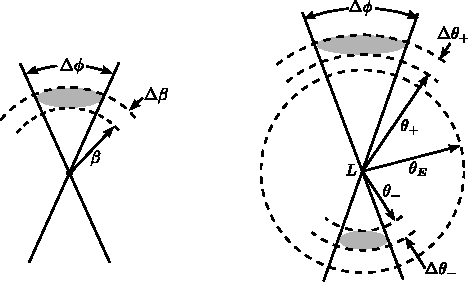
\includegraphics[width=0.6\textwidth]{../Images/Lensing_image_positions2.pdf}
				\caption[Schematic diagram of location of images]{Schematic diagram of location of images. The centre labelled L represents the observer-lens axis. The diagram on the left shows what would be observed if the lens was not present. The right hand diagram includes the effects of lensing\cite{Hartle}.\label{fig:Lensing_image_positions2}}
		\end{figure}

		In the case shown in Figure~\ref{fig:Lensing_image_positions2} where two visible images are observed, one image will form inside the Einstein radius ($\theta_{i+}$) and the other outside ($\theta_{i+}$). The positions of these two images are calculated by solving the Equation~\ref{eq:einstein_angle} giving
		\begin{align}
			\theta_{i\pm} &= \frac{1}{2}\left( \theta_S \pm {(\theta_S^2 + 4\theta_E^2)} ^{\frac{1}{2}} \right) \label{eq:image_position}
		\end{align}
		yielding the positions of the two unobstructed images as shown in Figure~\ref{fig:Lensing_image_positions2} one inside the Einstein radius, the other outside. Unlike optical lenses, gravitational lenses are achromatic, so the frequency of the light has no effect on the position of the images. As a result, images of the same object have exactly the same spectra and can easily be identified\cite{Hartle}.

		The azimuthal angle $\phi$ remains unchanged with and without the lens but as shown in figure lensing image positions, the polar angle and the width of the images are changed. The observed images are, therefore, stretched out into arcs and at any given radius will have the same curvature of a circle with origin at the centre of the lens\cite{Image_arc_curvature}. The change in the polar angle $\theta$ can be calculated by differentiating Equation~\ref{eq:image_position}, giving
		\begin{align}
			\Delta\theta_{i\pm} &= \frac{1}{2}\left( 1 \pm \frac{\theta_S}{(\theta_S^2 +4\theta_E^2)}^{\frac{1}{2}} \right) \Delta\theta_S
		\end{align}
		This shape distortion results from the fact that the sources are not point objects but in fact have light coming from a large area of the sky. The light from each end of the object will take different paths through the sky and will pass the lens at a different distance. The light will therefore be bent differently for different parts of the galaxy and the shape is distorted\cite{Arc_shapes_site}.

		The magnification of the source is given by the ratio of the image brightness to the source brightness. The surface brightness of any given source remains constant\cite{Hartle} but the effective solid angle $\Omega$ subtended by the detector is increased by the lens, hence the flux received by the detector, given by
		\begin{align}
			F &= (\text{surface brightness}) \times \Omega
		\end{align}
		is also increased. As the observed brightness of the source depends on the flux, the magnification is given by
		\begin{align}
			\mu &= \frac{F_{i\pm}}{F_S} = \frac{\Omega_{i\pm}}{\Omega_S}
			\intertext{Since in the small angle approximation, $\sin\theta \approx \theta$, the solid angles for the image and source are given by $\theta_{i\pm}\Delta\theta_{i\pm}\Delta\phi$ and $\theta_S \Delta_S \phi$ respectively. Given that $\Delta\phi$ is the same for both images, the magnification can be expressed as}
			\mu_{\pm} &= \left| \left( \frac{\theta_{i\pm}}{\theta_S} \dx{\theta_{i\pm}}{\theta_S} \right) \right| \\
			&=\frac{1}{4}\left( \frac{\theta_S}{{(\theta_S^2 +4\theta_E^2)}^{\frac{1}{2}}} + \frac{{(\theta_S^2 +4\theta_E^2)}^{\frac{1}{2}}}{\theta_S} \pm 2 \right)
			\intertext{For a lens modelled as a single isothermal sphere, this reduces to}
			\mu_\pm &= \frac{\theta_{i\pm}}{\theta_S} = \left( 1\mp \frac{\theta_E}{\theta_\pm} \right)^{-1}
		\end{align}
		The change in AB magnitude is then found using Equation~\ref{eq:magnitude_conversion}\cite{IOP_ABmagnification_site},
		\begin{align}
			\Delta m &= -2.5\log(\mu) \label{eq:magnitude_conversion}
		\end{align}
		The smaller the angle between the observer-lens axis and the source $\theta_S$, the greater the magnification of the source.
	% subsection concept (end)

% section gravitational_lensing (end)


% part general_theory (end)
\newpage
\part{Predictions} % (fold)
\label{prt:predictions}
    %!TEX root = mainfile.tex

\section{Predictions Group} % (fold)
\label{sec:predictions_group}
	In order for those attempting to observe high redshift galaxies to propose a detailed experimental plan, it is important to know how many galaxies one is expecting to observe within a certain volume of the sky. This is the fundamental purpose of the predictions sub-group; to be able to compute this quantity with the depth of the surveyed volume corresponding directly to redshift. In order to do this, a computer program is required to efficiently calculate this number as a function of redshift, field of view and apparent magnitude enabling those observing to make an informed prediction of the telescope one would need and the observing time required to make definitive observation of such elusive galaxies.

	This section of the project was structured chronologically as follows:
	\begin{itemize}
		\item Research how early galaxies are professionally predicted.
		\item Find a general Schechter function in terms of luminosity and/or magnitude.
		\item Mathematically process this function to ensure it is consistent with the units used by those carrying out the observations.
		\item Build a computer program to automate the process of calculating the number of galaxies from the Schechter function.
		\item Find plausible starting parameters to use in primary program.
		\item Collate parameter data from published papers.
		\item Determine parameter evolution with time.
		\item Plot these results to produce a visual description of how these parameters affect the outcome.
		\item Give expected number of galaxies to the observers.
		\item Refine technique with the inclusion of more advanced adaptations.
	\end{itemize}

	In addition to running a program to calculate the total number of galaxies, there is also a separate program to determine the redshifts at which re-ionization began and ended to be included when calculating the number of galaxies in the main code.

	The beginning of re-ionization has been determined by equating the star formation rate density with the critical star formation rate density required for matter to collapse into galaxies (see section..OWEN). The end of re-ionization occurs when the photons produced in star formation have completely ionized the IGM and hence required direct application of star formation rate densities also. This will be covered in more detail in section~\ref{sec:lower_redshift_limit_on_re-ionization}.

% section predictions_group (end)

    %!TEX root = mainfile.tex

\section{Cosmological Distances} % (fold)
\label{sec:cosmological_distances}
	This section introduces some of the important distances used in various prediction calculations. First of all is the comoving distance between two observers at different redshifts. This is calculated via equation~\ref{fig:comoving_distance}\cite{distance_measures_cosmology},
	\begin{align}
		D_{C}(z)=\frac{c}{H_{0}}\int^{z_{2}}_{z_{1}}\frac{\d{z'}}{E(z')} \label{fig:comoving_distance}
	\end{align}
	where $E(z)$ is the dimensionless Hubble parameter which is,
	\begin{align}
		E(z)=\sqrt{\Omega_{M}{(1+z)}^{3}+\Omega_{R}{(1+z)}^{4}+\Omega_{\Lambda}}
	\end{align}
	Where $\Omega_{M}$, $\Omega_{R}$ and $\Omega_{\Lambda}$ are the different density parameters for mass, radiation and dark energy respectively.

	To calculate the comoving distance to an object at a particular redshift the integral above must be done for $z_{1}=0$ up to an arbitrary $z$. Comoving distance is the distance between two comoving observers i.e.\ both moving with respect to the Hubble flow (factoring out the expansion of the universe). In the project this has been used to determine a volume of space for a given redshift range. This was done by finding the volume difference between two shells of comoving radius at two different redshifts.

	The luminosity distance is the distance that a photon travels from a source to an observer. As a photon will undergo a Doppler shift and be redshifted into longer wavelengths (red part of the spectrum). Therefore the luminosity distance is essentially a redshifted transverse comoving distance\cite{distance_measures_cosmology}, which for a flat universe is the comoving distance therefore,
	\begin{align}
		D_{L}(z)=(1+z)D_{C}(z)
	\end{align}
	In this project the luminosity distance has been used to convert between magnitudes, luminosity and flux.

	Also, the angular diameter distance is simply the proper distance along a radius $r_{e}$ where this is the radius at the time of emission. Therefore angular diameter distance is,
	\begin{align}
		D_{A} &= r_{e}a_{e} = \frac{a_{0}r_{e}}{1+z_{e}}
		\intertext{where $a_{0}r_{e}$ in a flat universe is the same as,}
		D_{A}(z) &= \frac{D_{C}}{1+z}
	\end{align}
	This is used to convert angular seperations in telescope images to actual angular seperations and then can determine the size of objects\cite{distance_measures_cosmology}.
% section cosmological_distances (end)

\section{Schechter Function} % (fold)
\label{sec:schechter_function}
	One important part of our project is to determine the luminosity function at high redshift, which is a plot of the number density of galaxies binned against their respective luminosities. A schechter function is used to fit this luminosity function. A schechter function is a form that has a power law which has a certain cut-off at which it becomes an exponential curve. The schechter function in terms of luminosity i.e.\ the luminosity function is shown in equation~\ref{eq:shechter_luminosity}\cite{cosmo_number_densities}.
	\begin{align}
		\phi(L)=\frac{\phi^{*}}{L^{*}}\frac{L}{L^{*}}^{\alpha}e^{-L/L^{*}} \label{eq:shechter_luminosity}
	\end{align}
	$\phi^{*}$ is the normalization factor in units of \si{\per\mega\parsec\cubed}, $\alpha$ is the gradient of the faint end slope of the luminosity function and $L^{*}$ is the characteristic luminosity at which the function changes from a power law to an exponential cut off. Therefore there are a majority of lower luminosity galaxies and not many bright ones.

	There are two basic methods to determine the best fit parameters of the schechter function\cite{luminosity_functions_online}. The first one is to take cluster samples and bin them by apparent magnitude then fit a schechter function trying to minimize the error. The other way is to use the ``maximum likelihood method''. This method takes a flux limited sample and finds the probability that a galaxy actually has a particular luminiostity at respective distances and then define a likelihood function which is the joint probability of finding all luminosities at their respective distances. These are then the most likely parameters consistent with the data and a schechter form. However in this project schechter parameters were simply cited from various articles as we are not doing any observations ourselves to get our predictions.

	The luminosity function can then be integrated to find the number density in \si{\per\mega\parsec\cubed},
	\begin{align}
		\rho_{N}=\int^{\infty}_{L}\phi(L)\d{L}
	\end{align}
	Where $L$ is the lower limit luminosity that can be seen in the universe, this is needed as the luminosity function tends to infinity at the faint end.

	It is easier to plot the luminosity function on the log scale and therefore most of the papers we cite state the absolute magnitude schechter function instead which is obtained by substituting,
	\begin{align}
		\frac{L}{L*}=10^{0.4(M^{*}-M)}
	\end{align}
	which is then multiplied by the derivative and rearranged to get the equation,
	\begin{align}
		\phi(M)=\phi^{*}(\ln(10)){\left[10^{0.4(M^{*}-M)}\right]}^{\alpha+1}\e{\left[-10^{0.4(M^{*}-M)}\right]}
	\end{align}
	Where $M^{*}$ is the characteristic absolute magnitude where the cut off happens.

	However a range of apparent magnitudes is normally observed, rather than absolute magnitudes and so the absolute magnitude equation above is changed to it's apparent magnitude form, using the simple relationship below,
	\begin{align}
		m=M+5((\log_{10}D_{L})-1)
	\end{align}
	Where $D_{L}$ is the luminosity distance. Note that the derivative of this substitution is 1 and so does not need to be accounted for.

	Or the luminosity density of galaxies in \si{\erg\per\second\per\mega\parsec\cubed\per\hertz} can also be calculated using,
	\begin{align}
		\rho_{L}=\int^{\infty}_{L}L\phi(L)dL
	\end{align}
	This will become useful for calculating star formation rates in later sections.
% section schechter_function (end)

\section{Lower Redshift limit on Re-ionization} % (fold)
\label{sec:lower_redshift_limit_on_re-ionization}
	In the project the way that the lower redshift limit has been calculated is to first calculate the rate of photons capable of ionizing a hydrogen atom via equation~\ref{eq:rate_of_ionising_photons}\cite{2010Natur.468...49R}.
	\begin{align}
		\frac{\d{n_{ion}}}{\d{t}}=f_{esc}\zeta\rho_\text{SFR}\label{eq:rate_of_ionising_photons}
	\end{align}
	Where $f_{esc}$ is the fraction of ionizing photons that escape a galaxy, $\zeta$ is the number of hydrogen-ionizing photons produced per second per unit star formation rate and $\rho_\text{SFR}$ is the star formation rate per unit volume.

	Therefore by integrating this equation up to the age of the universe at a specific redshift a total number of photons capable of ionizing the universe can be outputted. The number of ionizing photons are then equated to the total number of hydrogen atoms in the IGM of the universe to get a lower redshift limit of re-ionization.

	First of all the program gets the critical density of the universe by,
	\begin{align}
		\rho_{crit}(z)=\frac{3H{(z)}^{2}}{8\pi G}
	\end{align}
	Then by multiplying this by the baryonic density parameter, $\Omega_{b}=0.045\pm0.004$, the baryonic density is achieved. By then multiplying by the fraction of hydrogen, calculated from big bang nucleosynthesis, the total density of hydrogen in the universe can be obtained.

	From the 7 year WMAP survey\cite{2011ApJS..192...18K}, we can get the primordial Helium fraction to be $Y=0.33\pm0.09$. Where we assume that Hydrogen fraction ($X$) is simply $1-Y$ (therefore 0 metallicity). Although a simplifying assumption it is not too bad as the errors on fraction of helium are higher than the actual fraction of heavier elements.

	Then finally dividing the mass density of hydrogen by the atomic mass unit the code obtains a number density of hydrogen. In the code a redshift time relation $\frac{1}{(1+z)}\propto t^{2/3}$, assuming a matter dominated universe, is used and therefore,
	\begin{align}
		t &= \frac{t_{0}}{{(1+z)}^{3/2}} \\
		\Rightarrow \dx{t}{z} &= \frac{3}{2}\frac{t_{0}}{{(1+z)}^{5/2}}
	\end{align}

	In the first version of the code, values of star formation rate densities from  various articles with redshifts varying from redshifts 4 to up to about 8 from\cite{2010MNRAS.401.2561W}, which determine star formation rates from observations of Gamma-ray bursts (GRBs) from deaths of massive short lived stars which can be directly related to star formation rate. Also compiling these values with those from\cite{2012ApJ...759L..38A}, which use a semi-analytical model to determine star formation rates from redshifts 9 to 16. These two papers with very different methods have surprising correlation in values.

	These values were then plotted against redshift. The function of redshift that was used for $\rho_\text{SFR}$ was,
	\begin{align}
		\rho_\text{SFR}(z)=0.399(\pm 0.181)\e{-0.253(\pm 0.118)z}-0.011(\pm 0.025)
	\end{align}
	However this equation will only work up to a redshift of around 5 as the star formation rate for galaxies will drop with redshifts lower than this due to the gas being used up and star formation will drop off. This should not effect our results too much however as the project tends to study redshifts higher than this anyway. Also there will be large errors on higher redshift values due to problems with extrapolating the data, and unrealistic numbers of star formation where in reality there would be none.
	%Reference to beth's section
	We also used rough estimates of $f_\text{esc}=0.2$ and $\zeta=10^{53.5}$ as stated in section~\ref{???}.

	The code also used a function of the global stellar mass density to figure out the amount of hydrogen that was calculated was in stars at a given redshift. This therefore gives us a certain fraction that is not part of the IGM and does not need to be ionized. These values were taken from the direct observations of three papers \cite{2006A&A...459..745F}, \cite{2003A&A...401...73W} and \cite{2003ApJS..149..289B}. The function of redshift that was calculated was,
	\begin{align}
		\rho_\text{stellar}(M_{\odot}\si{\per\mega\parsec\cubed})=\e{-0.81z+19.7}
	\end{align}
	but this does not have much effect on the number of hydrogen as the stellar fraction is very small, so this is not a significant contributing factor.

	The code then loops for different values of redshift from redshift 25 at redshift intervals of 0.1, calculating the number of ionizing photons at those different epochs and equating this to the hydrogen number. This then outputs ionized fraction against redshift, shown in figure \ref{fig:IonizedFraction1}.
	\begin{figure}[!htb]
		\centering
			\begingroup\endlinechar=-1
		  		\resizebox{0.7\textwidth}{!}{%
					% GNUPLOT: LaTeX picture with Postscript
\begingroup
  \makeatletter
  \providecommand\color[2][]{%
    \GenericError{(gnuplot) \space\space\space\@spaces}{%
      Package color not loaded in conjunction with
      terminal option `colourtext'%
    }{See the gnuplot documentation for explanation.%
    }{Either use 'blacktext' in gnuplot or load the package
      color.sty in LaTeX.}%
    \renewcommand\color[2][]{}%
  }%
  \providecommand\includegraphics[2][]{%
    \GenericError{(gnuplot) \space\space\space\@spaces}{%
      Package graphicx or graphics not loaded%
    }{See the gnuplot documentation for explanation.%
    }{The gnuplot epslatex terminal needs graphicx.sty or graphics.sty.}%
    \renewcommand\includegraphics[2][]{}%
  }%
  \providecommand\rotatebox[2]{#2}%
  \@ifundefined{ifGPcolor}{%
    \newif\ifGPcolor
    \GPcolortrue
  }{}%
  \@ifundefined{ifGPblacktext}{%
    \newif\ifGPblacktext
    \GPblacktexttrue
  }{}%
  % define a \g@addto@macro without @ in the name:
  \let\gplgaddtomacro\g@addto@macro
  % define empty templates for all commands taking text:
  \gdef\gplbacktext{}%
  \gdef\gplfronttext{}%
  \makeatother
  \ifGPblacktext
    % no textcolor at all
    \def\colorrgb#1{}%
    \def\colorgray#1{}%
  \else
    % gray or color?
    \ifGPcolor
      \def\colorrgb#1{\color[rgb]{#1}}%
      \def\colorgray#1{\color[gray]{#1}}%
      \expandafter\def\csname LTw\endcsname{\color{white}}%
      \expandafter\def\csname LTb\endcsname{\color{black}}%
      \expandafter\def\csname LTa\endcsname{\color{black}}%
      \expandafter\def\csname LT0\endcsname{\color[rgb]{1,0,0}}%
      \expandafter\def\csname LT1\endcsname{\color[rgb]{0,1,0}}%
      \expandafter\def\csname LT2\endcsname{\color[rgb]{0,0,1}}%
      \expandafter\def\csname LT3\endcsname{\color[rgb]{1,0,1}}%
      \expandafter\def\csname LT4\endcsname{\color[rgb]{0,1,1}}%
      \expandafter\def\csname LT5\endcsname{\color[rgb]{1,1,0}}%
      \expandafter\def\csname LT6\endcsname{\color[rgb]{0,0,0}}%
      \expandafter\def\csname LT7\endcsname{\color[rgb]{1,0.3,0}}%
      \expandafter\def\csname LT8\endcsname{\color[rgb]{0.5,0.5,0.5}}%
    \else
      % gray
      \def\colorrgb#1{\color{black}}%
      \def\colorgray#1{\color[gray]{#1}}%
      \expandafter\def\csname LTw\endcsname{\color{white}}%
      \expandafter\def\csname LTb\endcsname{\color{black}}%
      \expandafter\def\csname LTa\endcsname{\color{black}}%
      \expandafter\def\csname LT0\endcsname{\color{black}}%
      \expandafter\def\csname LT1\endcsname{\color{black}}%
      \expandafter\def\csname LT2\endcsname{\color{black}}%
      \expandafter\def\csname LT3\endcsname{\color{black}}%
      \expandafter\def\csname LT4\endcsname{\color{black}}%
      \expandafter\def\csname LT5\endcsname{\color{black}}%
      \expandafter\def\csname LT6\endcsname{\color{black}}%
      \expandafter\def\csname LT7\endcsname{\color{black}}%
      \expandafter\def\csname LT8\endcsname{\color{black}}%
    \fi
  \fi
  \setlength{\unitlength}{0.0500bp}%
  \begin{picture}(7200.00,4320.00)%
    \gplgaddtomacro\gplbacktext{%
      \put(747,595){\makebox(0,0)[r]{\strut{} 0}}%
      \put(747,1182){\makebox(0,0)[r]{\strut{} 0.2}}%
      \put(747,1768){\makebox(0,0)[r]{\strut{} 0.4}}%
      \put(747,2355){\makebox(0,0)[r]{\strut{} 0.6}}%
      \put(747,2942){\makebox(0,0)[r]{\strut{} 0.8}}%
      \put(747,3528){\makebox(0,0)[r]{\strut{} 1}}%
      \put(747,4115){\makebox(0,0)[r]{\strut{} 1.2}}%
      \put(849,409){\makebox(0,0){\strut{} 0}}%
      \put(2058,409){\makebox(0,0){\strut{} 5}}%
      \put(3267,409){\makebox(0,0){\strut{} 10}}%
      \put(4475,409){\makebox(0,0){\strut{} 15}}%
      \put(5684,409){\makebox(0,0){\strut{} 20}}%
      \put(6893,409){\makebox(0,0){\strut{} 25}}%
      \csname LTb\endcsname%
      \put(144,2355){\rotatebox{-270}{\makebox(0,0){\strut{}Ionised Fraction ($X$)}}}%
      \csname LTb\endcsname%
      \put(3871,130){\makebox(0,0){\strut{}Redshift (z)}}%
      \put(3871,4022){\makebox(0,0){\strut{}}}%
    }%
    \gplgaddtomacro\gplfronttext{%
      \csname LTb\endcsname%
      \put(6105,3948){\makebox(0,0)[r]{\strut{}Best Fit}}%
      \csname LTb\endcsname%
      \put(6105,3762){\makebox(0,0)[r]{\strut{}Lower Limit}}%
      \csname LTb\endcsname%
      \put(6105,3576){\makebox(0,0)[r]{\strut{}Upper Limit}}%
    }%
    \gplbacktext
    \put(0,0){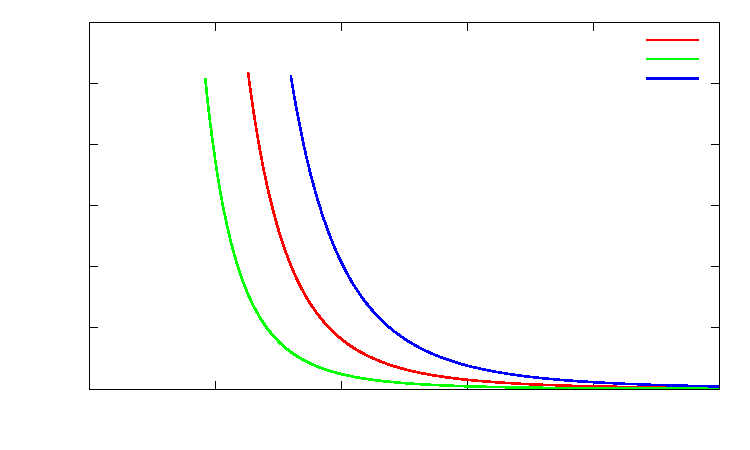
\includegraphics{GRAPH_StellarDens_exponential}}%
    \gplfronttext
  \end{picture}%
\endgroup

		  		}\endgroup
		\caption{Plot of modeled ionized fraction of the IGM as a function of redshift.\label{fig:IonizedFraction1}}
	\end{figure}

	From this we get that the universe is completely ionized at a redshift $6.3\pm1.7$, ignoring the rather large errors, this number is not a bad estimate of the epoch. We know this from articles which show from observations of Lyman-$\alpha$ emitters that there must be a large ionized fraction at 6.5, due to attenuation from neutral hydrogen\cite{Ota:arXiv0707.1561}. Various theoretical models of star formation rate predict a ionized universe at around 6 and it is stated that the Sunyaev-Zeldovich effect has put a limit that Reionization ends earlier than 5.8 \cite{2012MNRAS.423..862K}.

	However as recombination has not been included which will slow down the rate at which the universe is ionized or the fact that both the escape fraction and $\zeta$ are likely to change with redshift, this number is not actually realistic.

	\subsection{Evolving Escape Fraction} % (fold)
	\label{sub:evolving_escape_fraction}
		As already stated the previous results make a basic assumption of of the escape fraction to be about $20\%$ during the epoch of reionization. This is obviously not a very good assumption as it will evolve with redshift. However there lies a problem in this which is related to the previous section, section~\ref{???}(Beth's bit on fesc) which explained the difficulty in measuring this parameter as well as the problems in extrapolating out to higher redshifts much like in our star formation rates. This uncertainty in the measure is what leads to the differences stated in\cite{2012ApJ...759L..38A}, which states a higher fraction at higher redshift due to lack of dust, and\cite{2000ApJ...545...86W} which states the opposite, due to increasing disk densities and increasing density in the universe as a whole. However from\cite{2012arXiv1209.2123F} and\cite{2013MNRAS.428L...1M} by using recent semi-analytical model they found that the escape fraction does indeed increase with redshift and so this is the model that is used in this project.

		Once again using the fit program to fit a exponential to the escape fraction measurements and predictions from\cite{2012ApJ...759L..38A},\cite{2006ApJ...651L..89R} and\cite{2006MNRAS.371L...1I}. The functional form that is achieved is,
		\begin{align}
			f_\text{esc}(z)=\e{0.013\pm0.011-0.952\pm0.06}
		\end{align}
		The code is then run again with this escape fraction instead of the constant $20\%$, the results achieved are shown in \ref{fig:IonizedFraction2}
		\begin{figure}
			\centering
				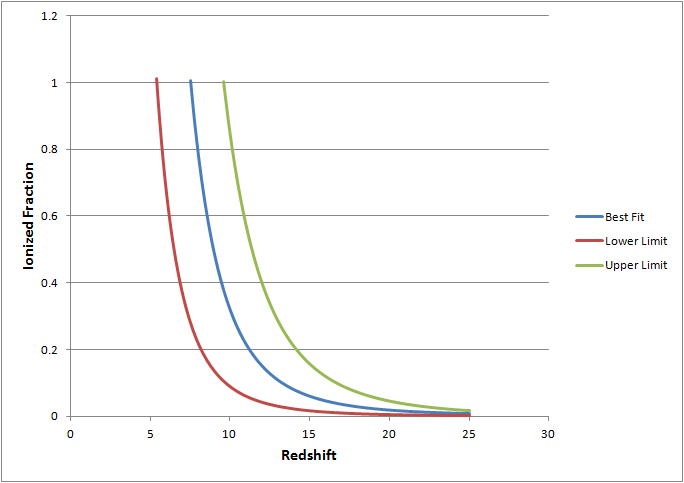
\includegraphics[width=0.8\textwidth]{F:/Extragalactic cosmology/IonizedFraction2.png}
				\caption{Plot of modeled ionized fraction of the IGM as a function of redshift with predicting evolving escape fraction.\label{fig:IonizedFraction2}}
		\end{figure}

		The graph in figure~\ref{fig:IonizedFraction2} shows that the addition of the evolving escape fraction has resulted in the universe being ionized quicker which is what is expected, since recombinations have not been included in this model. This model outputs a redshift of $7.5\pm2.1$, which shows the increase in redshift and also in error due to the error on $f_\text{esc}$ itself. It is very hard to determine whether this is an improvement or a hindrance to the previous model just due to the errors on measuring/predicting f_{esc}.

		%Not completed having trouble with it not sure if it should be included without conclusive results?
	% subsection evolving_escape_fraction (end)

	\subsection{Recombinations} % (fold)
	\label{sub:recombinations}
		To include Recombinations into our project, the rate at which hydrogen will recombine. The mean recombination time was found in \cite{2012MNRAS.423..862K} to be,
		\begin{align}
			\bar{t}_\text{rec} &= \frac{1}{C_{HII}\alpha_{B}(T_{0})\bar{n}_{H}(1+Y/4X)(1+z)^{3}}\\
			&\approx 0.93Gyr\left(\frac{3}{C_{HII}}\right)\left(\frac{T_{0}}{2\times 10^{4}K}\right)^{0.7}\left(\frac{7}{1+z}\right)^{3}
		\end{align}
		Where $C_{HII}$ is the clumping factor of ionized hydrogen and $T_{0}$ is the mean IGM temperature. Both of these values are plotted and fitted against redshift exactly in the same way as previous parameters. Where values of the clumping factor against redshift are cited from a theoretical model in\cite{2011MNRAS.412L..16R} and the IGM mean temperature is cited from\cite{2006MNRAS.373.1265O} based on simulations.

		The code then takes this equation for the mean recombination time of hydrogen and integrates the inverse of this from 0 to the specific $t(z)$. This will give us a mean total of hydrogen that will have recombined in that time period. However when this method is implemented into the code and ran, it outputs values of recombination that are insignificant because they are so low. This seems unphysical as we would expect the recombinations in the universe to be much higher than this and make a significant contribution to the rate at which the universe ionizes.
	% subsection recombinations (end)

% section lower_redshift_limit_on_re-ionization (end)

    %!TEX root = mainfile.tex

\section{Assumptions Made} % (fold)
\label{sec:assumptions_made}
	The mathematical model that will be used in our program is limited by certain assumptions about the universe that we are working in. Some of these are generally held to be true and are accepted widely in the scientific community, others are due to the constraints of what we can mathematically program and the observational data available from previous studies. A major assumption that we are making throughout our work on re-ionisation concerns the type of universe that we exist in. A related pair of assumptions which have firm mathematical basis are the ``Cosmological Principle'' and the ``Isotropic Universe Theorem''. These state that our observations, as made from the Earth, are not subject to any influence from our location within it, in other words, we are not in a privileged position in the universe. This is assumed for almost all cosmological studies and shall not be considered.

	An important assumption that we are forced to make is that the Schechter function that we use describes our universe sufficiently to make predictions from. This is not as trivial as it sounds since the function is derived from data collected from much lower redshifts than some that we are considering. Further data will allow the accuracy of these functions to be improved. We have collected data and mathematical contributions from a number of high redshift studies to attempt to reduce the possibility of error and increase the accuracy of our function to as high a redshift as possible.

	For the early stages of our investigation, we will assume that both parameter evolution and cosmic variance do not influence the results. Clearly, these are big assumptions to make and so will be integrated into the calculations at later stages. This will be discussed further later.

	\subsubsection{AB Magnitude} % (fold)
	\label{ssub:ab_magnitude}
		In order to keep consistancy between the parts of this project, we have used the AB magnitude system throughout. This is a system for measuring the magnutide of an object in the sky. It is defined as
		\begin{align}
			M(AB) &= -2.5\log(f_\nu) -48.60
		\end{align}
		where $f_\nu$ is the monochormatic flux measured in \si{\erg\per\second\per\square\centi\metre\per\hertz}.
	% subsubsection ab_magnitude (end)

% section assumptions_made (end)

    %!TEX root = mainfile.tex

\section{Parameter Values} % (fold)
\label{sec:parameter_values}
    There are also a number of parameters in the Schechter function that must be specified. In order to find suitable values to use, we collected data from a number of different sources covering several studies. All of the studies that have been performed in the past concern galaxies at lower redshifts than we are expecting to examine. To get an estimate for the value of each of the parameters at higher redshift, the values found were plotted and the fit extrapolated to cover the era necessary. Since some of the fits demonstrate that these parameters are not constant with time, their evolution shall be incorporated into the calculations.

    The values in the Schechter function that we have determined fits for are $\alpha$, $M^{*}$ and $\phi^{*}$. The data collected for each of these fits is shown in appendix~\ref{app:parameter_fit_data}.

    \subsection{Parameter Evolution} % (fold)
    \label{sub:parameter_evolution}
        The early stages of the models we used assumed that the parameters of the Schechter function were static with respect to time. This means that, when iterating over the redshift, the only property that changed was the co-moving volume. This is non-physical since it does not allow for changes in the characteristic mass and characteristic luminosity for different conditions in the universe. In order to improve the model, we collected data from a number of previous studies for three values, the characteristic mass, $M^*$, the Schechter normalisation, $\phi^*$ and the faint end slope parameter, $\alpha$.

        \subsubsection{Linear Parameter Evolution with Redshift} % (fold)
        \label{ssub:linear_parameter_evolution_with_redshift}

            In order to provide useful errors on the fits of the parameters, a technique called the pivot fit method is used to decouple the errors on $y$-intercept and gradient. This involved fitting the data after it has been normalised around the mean value. This normalisation simply involves taking the mean $x$- and $y$-value from each data point so that the graph is centred about the origin. This means that the $y$-intercept is fixed to zero and thus the fitting error applies only to the gradient. Subsequent linear fits shall be treated in this manner, so that errors quoted correspond to the gradient. For clarity of presentation, the data shall be plotted in its original form.

            The graph in figure~\ref{fig:alpha_evolution} shows the data collected, with the corresponding uncertainties, for the linear parameter, $\alpha$. From this data, a linear fit is taken. The relevant evolution, then, is governed by the equation $\alpha = -0.015z - 1.664$.
            \begin{figure}[!htb]
                \centering
                    \begingroup\endlinechar=-1
                        \resizebox{0.6\textwidth}{!}{%
                            % GNUPLOT: LaTeX picture with Postscript
\begingroup
  \makeatletter
  \providecommand\color[2][]{%
    \GenericError{(gnuplot) \space\space\space\@spaces}{%
      Package color not loaded in conjunction with
      terminal option `colourtext'%
    }{See the gnuplot documentation for explanation.%
    }{Either use 'blacktext' in gnuplot or load the package
      color.sty in LaTeX.}%
    \renewcommand\color[2][]{}%
  }%
  \providecommand\includegraphics[2][]{%
    \GenericError{(gnuplot) \space\space\space\@spaces}{%
      Package graphicx or graphics not loaded%
    }{See the gnuplot documentation for explanation.%
    }{The gnuplot epslatex terminal needs graphicx.sty or graphics.sty.}%
    \renewcommand\includegraphics[2][]{}%
  }%
  \providecommand\rotatebox[2]{#2}%
  \@ifundefined{ifGPcolor}{%
    \newif\ifGPcolor
    \GPcolortrue
  }{}%
  \@ifundefined{ifGPblacktext}{%
    \newif\ifGPblacktext
    \GPblacktexttrue
  }{}%
  % define a \g@addto@macro without @ in the name:
  \let\gplgaddtomacro\g@addto@macro
  % define empty templates for all commands taking text:
  \gdef\gplbacktext{}%
  \gdef\gplfronttext{}%
  \makeatother
  \ifGPblacktext
    % no textcolor at all
    \def\colorrgb#1{}%
    \def\colorgray#1{}%
  \else
    % gray or color?
    \ifGPcolor
      \def\colorrgb#1{\color[rgb]{#1}}%
      \def\colorgray#1{\color[gray]{#1}}%
      \expandafter\def\csname LTw\endcsname{\color{white}}%
      \expandafter\def\csname LTb\endcsname{\color{black}}%
      \expandafter\def\csname LTa\endcsname{\color{black}}%
      \expandafter\def\csname LT0\endcsname{\color[rgb]{1,0,0}}%
      \expandafter\def\csname LT1\endcsname{\color[rgb]{0,1,0}}%
      \expandafter\def\csname LT2\endcsname{\color[rgb]{0,0,1}}%
      \expandafter\def\csname LT3\endcsname{\color[rgb]{1,0,1}}%
      \expandafter\def\csname LT4\endcsname{\color[rgb]{0,1,1}}%
      \expandafter\def\csname LT5\endcsname{\color[rgb]{1,1,0}}%
      \expandafter\def\csname LT6\endcsname{\color[rgb]{0,0,0}}%
      \expandafter\def\csname LT7\endcsname{\color[rgb]{1,0.3,0}}%
      \expandafter\def\csname LT8\endcsname{\color[rgb]{0.5,0.5,0.5}}%
    \else
      % gray
      \def\colorrgb#1{\color{black}}%
      \def\colorgray#1{\color[gray]{#1}}%
      \expandafter\def\csname LTw\endcsname{\color{white}}%
      \expandafter\def\csname LTb\endcsname{\color{black}}%
      \expandafter\def\csname LTa\endcsname{\color{black}}%
      \expandafter\def\csname LT0\endcsname{\color{black}}%
      \expandafter\def\csname LT1\endcsname{\color{black}}%
      \expandafter\def\csname LT2\endcsname{\color{black}}%
      \expandafter\def\csname LT3\endcsname{\color{black}}%
      \expandafter\def\csname LT4\endcsname{\color{black}}%
      \expandafter\def\csname LT5\endcsname{\color{black}}%
      \expandafter\def\csname LT6\endcsname{\color{black}}%
      \expandafter\def\csname LT7\endcsname{\color{black}}%
      \expandafter\def\csname LT8\endcsname{\color{black}}%
    \fi
  \fi
  \setlength{\unitlength}{0.0500bp}%
  \begin{picture}(7200.00,4320.00)%
    \gplgaddtomacro\gplbacktext{%
      \put(747,915){\makebox(0,0)[r]{\strut{}-2.2}}%
      \put(747,1555){\makebox(0,0)[r]{\strut{}-2}}%
      \put(747,2195){\makebox(0,0)[r]{\strut{}-1.8}}%
      \put(747,2835){\makebox(0,0)[r]{\strut{}-1.6}}%
      \put(747,3475){\makebox(0,0)[r]{\strut{}-1.4}}%
      \put(747,4115){\makebox(0,0)[r]{\strut{}-1.2}}%
      \put(849,409){\makebox(0,0){\strut{} 0}}%
      \put(2058,409){\makebox(0,0){\strut{} 2}}%
      \put(3267,409){\makebox(0,0){\strut{} 4}}%
      \put(4475,409){\makebox(0,0){\strut{} 6}}%
      \put(5684,409){\makebox(0,0){\strut{} 8}}%
      \put(6893,409){\makebox(0,0){\strut{} 10}}%
      \csname LTb\endcsname%
      \put(144,2355){\rotatebox{-270}{\makebox(0,0){\strut{}Faint End Slope ($\alpha$)}}}%
      \csname LTb\endcsname%
      \put(3871,130){\makebox(0,0){\strut{}Redshift ($z$)}}%
      \put(3871,4022){\makebox(0,0){\strut{}}}%
    }%
    \gplgaddtomacro\gplfronttext{%
      \csname LTb\endcsname%
      \put(3297,762){\makebox(0,0)[r]{\strut{}$f(x) = -0.015x + -1.664$}}%
    }%
    \gplbacktext
    \put(0,0){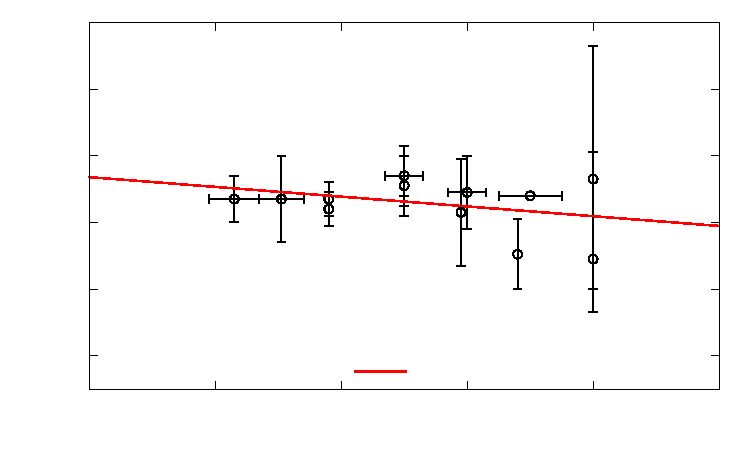
\includegraphics{GRAPH_Parameter_Fit_alpha_linear}}%
    \gplfronttext
  \end{picture}%
\endgroup

                        }\endgroup
                \caption{The evolution of $\alpha$ as a function of redshift according to past observational studies.\label{fig:alpha_evolution}}
            \end{figure}

            Figure~\ref{fig:phi_evolution} shows the data for the evolution of the normalisation parameter $\phi^{*}$. This value is known to be never less than zero. For this reason, coupled with an attempt to reduce the errors as far as possible, an exponential decrease with redshift was chosen. Although the errors for this fit are large, because of the errors on the data points, the region of concern, high redshift greater than 6, this evolution can be approximated to zero. In other words, during the times that we are considering, it can be approximated that there was no change in the value of the normalisation parameter, $\phi^*$.
            \begin{figure}[!htb]
                \centering
                    \begingroup\endlinechar=-1
                        \resizebox{0.6\textwidth}{!}{%
                            % GNUPLOT: LaTeX picture with Postscript
\begingroup
  \makeatletter
  \providecommand\color[2][]{%
    \GenericError{(gnuplot) \space\space\space\@spaces}{%
      Package color not loaded in conjunction with
      terminal option `colourtext'%
    }{See the gnuplot documentation for explanation.%
    }{Either use 'blacktext' in gnuplot or load the package
      color.sty in LaTeX.}%
    \renewcommand\color[2][]{}%
  }%
  \providecommand\includegraphics[2][]{%
    \GenericError{(gnuplot) \space\space\space\@spaces}{%
      Package graphicx or graphics not loaded%
    }{See the gnuplot documentation for explanation.%
    }{The gnuplot epslatex terminal needs graphicx.sty or graphics.sty.}%
    \renewcommand\includegraphics[2][]{}%
  }%
  \providecommand\rotatebox[2]{#2}%
  \@ifundefined{ifGPcolor}{%
    \newif\ifGPcolor
    \GPcolortrue
  }{}%
  \@ifundefined{ifGPblacktext}{%
    \newif\ifGPblacktext
    \GPblacktexttrue
  }{}%
  % define a \g@addto@macro without @ in the name:
  \let\gplgaddtomacro\g@addto@macro
  % define empty templates for all commands taking text:
  \gdef\gplbacktext{}%
  \gdef\gplfronttext{}%
  \makeatother
  \ifGPblacktext
    % no textcolor at all
    \def\colorrgb#1{}%
    \def\colorgray#1{}%
  \else
    % gray or color?
    \ifGPcolor
      \def\colorrgb#1{\color[rgb]{#1}}%
      \def\colorgray#1{\color[gray]{#1}}%
      \expandafter\def\csname LTw\endcsname{\color{white}}%
      \expandafter\def\csname LTb\endcsname{\color{black}}%
      \expandafter\def\csname LTa\endcsname{\color{black}}%
      \expandafter\def\csname LT0\endcsname{\color[rgb]{1,0,0}}%
      \expandafter\def\csname LT1\endcsname{\color[rgb]{0,1,0}}%
      \expandafter\def\csname LT2\endcsname{\color[rgb]{0,0,1}}%
      \expandafter\def\csname LT3\endcsname{\color[rgb]{1,0,1}}%
      \expandafter\def\csname LT4\endcsname{\color[rgb]{0,1,1}}%
      \expandafter\def\csname LT5\endcsname{\color[rgb]{1,1,0}}%
      \expandafter\def\csname LT6\endcsname{\color[rgb]{0,0,0}}%
      \expandafter\def\csname LT7\endcsname{\color[rgb]{1,0.3,0}}%
      \expandafter\def\csname LT8\endcsname{\color[rgb]{0.5,0.5,0.5}}%
    \else
      % gray
      \def\colorrgb#1{\color{black}}%
      \def\colorgray#1{\color[gray]{#1}}%
      \expandafter\def\csname LTw\endcsname{\color{white}}%
      \expandafter\def\csname LTb\endcsname{\color{black}}%
      \expandafter\def\csname LTa\endcsname{\color{black}}%
      \expandafter\def\csname LT0\endcsname{\color{black}}%
      \expandafter\def\csname LT1\endcsname{\color{black}}%
      \expandafter\def\csname LT2\endcsname{\color{black}}%
      \expandafter\def\csname LT3\endcsname{\color{black}}%
      \expandafter\def\csname LT4\endcsname{\color{black}}%
      \expandafter\def\csname LT5\endcsname{\color{black}}%
      \expandafter\def\csname LT6\endcsname{\color{black}}%
      \expandafter\def\csname LT7\endcsname{\color{black}}%
      \expandafter\def\csname LT8\endcsname{\color{black}}%
    \fi
  \fi
  \setlength{\unitlength}{0.0500bp}%
  \begin{picture}(7200.00,4320.00)%
    \gplgaddtomacro\gplbacktext{%
      \put(1053,595){\makebox(0,0)[r]{\strut{} 0}}%
      \put(1053,947){\makebox(0,0)[r]{\strut{} 0.0005}}%
      \put(1053,1299){\makebox(0,0)[r]{\strut{} 0.001}}%
      \put(1053,1651){\makebox(0,0)[r]{\strut{} 0.0015}}%
      \put(1053,2003){\makebox(0,0)[r]{\strut{} 0.002}}%
      \put(1053,2355){\makebox(0,0)[r]{\strut{} 0.0025}}%
      \put(1053,2707){\makebox(0,0)[r]{\strut{} 0.003}}%
      \put(1053,3059){\makebox(0,0)[r]{\strut{} 0.0035}}%
      \put(1053,3411){\makebox(0,0)[r]{\strut{} 0.004}}%
      \put(1053,3763){\makebox(0,0)[r]{\strut{} 0.0045}}%
      \put(1053,4115){\makebox(0,0)[r]{\strut{} 0.005}}%
      \put(1155,409){\makebox(0,0){\strut{} 0}}%
      \put(2303,409){\makebox(0,0){\strut{} 2}}%
      \put(3450,409){\makebox(0,0){\strut{} 4}}%
      \put(4598,409){\makebox(0,0){\strut{} 6}}%
      \put(5745,409){\makebox(0,0){\strut{} 8}}%
      \put(6893,409){\makebox(0,0){\strut{} 10}}%
      \csname LTb\endcsname%
      \put(144,2355){\rotatebox{-270}{\makebox(0,0){\strut{}Normalisation ($\phi^{*}$)}}}%
      \csname LTb\endcsname%
      \put(4024,130){\makebox(0,0){\strut{}Redshift ($z$)}}%
      \put(4024,4022){\makebox(0,0){\strut{}}}%
    }%
    \gplgaddtomacro\gplfronttext{%
      \csname LTb\endcsname%
      \put(6105,3948){\makebox(0,0)[r]{\strut{}$f(x) = 0.052e^{-1.487x} + 0.001$}}%
    }%
    \gplbacktext
    \put(0,0){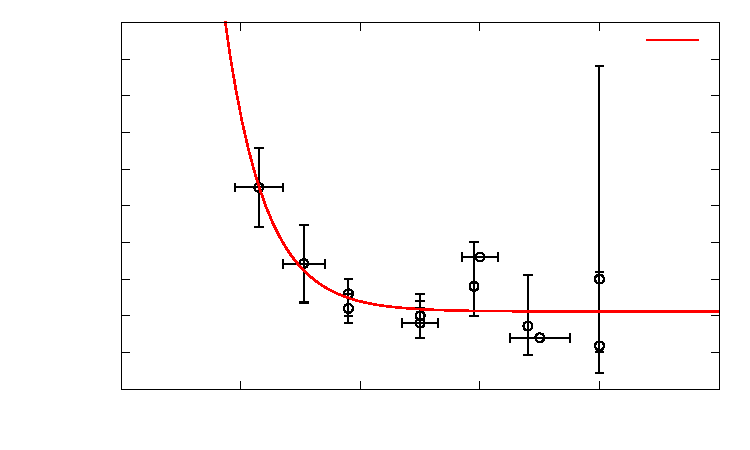
\includegraphics{GRAPH_Parameter_Fit_phi-star_exponential}}%
    \gplfronttext
  \end{picture}%
\endgroup

                        }\endgroup
                \caption{The evolution of $\phi^{*}$ as a function of redshift according to past observational studies.\label{fig:phi_evolution}}
            \end{figure}

            The final parameter is the characteristic magnitude, $M^*$. It was determined that a linear fit was best again and so the pivot method was used to reduce the error. The final equation used was $M^* = 0.221z - 21.642$.
            \begin{figure}[!htb]
                \centering
                    \begingroup\endlinechar=-1
                        \resizebox{0.6\textwidth}{!}{%
                            % GNUPLOT: LaTeX picture with Postscript
\begingroup
  \makeatletter
  \providecommand\color[2][]{%
    \GenericError{(gnuplot) \space\space\space\@spaces}{%
      Package color not loaded in conjunction with
      terminal option `colourtext'%
    }{See the gnuplot documentation for explanation.%
    }{Either use 'blacktext' in gnuplot or load the package
      color.sty in LaTeX.}%
    \renewcommand\color[2][]{}%
  }%
  \providecommand\includegraphics[2][]{%
    \GenericError{(gnuplot) \space\space\space\@spaces}{%
      Package graphicx or graphics not loaded%
    }{See the gnuplot documentation for explanation.%
    }{The gnuplot epslatex terminal needs graphicx.sty or graphics.sty.}%
    \renewcommand\includegraphics[2][]{}%
  }%
  \providecommand\rotatebox[2]{#2}%
  \@ifundefined{ifGPcolor}{%
    \newif\ifGPcolor
    \GPcolortrue
  }{}%
  \@ifundefined{ifGPblacktext}{%
    \newif\ifGPblacktext
    \GPblacktexttrue
  }{}%
  % define a \g@addto@macro without @ in the name:
  \let\gplgaddtomacro\g@addto@macro
  % define empty templates for all commands taking text:
  \gdef\gplbacktext{}%
  \gdef\gplfronttext{}%
  \makeatother
  \ifGPblacktext
    % no textcolor at all
    \def\colorrgb#1{}%
    \def\colorgray#1{}%
  \else
    % gray or color?
    \ifGPcolor
      \def\colorrgb#1{\color[rgb]{#1}}%
      \def\colorgray#1{\color[gray]{#1}}%
      \expandafter\def\csname LTw\endcsname{\color{white}}%
      \expandafter\def\csname LTb\endcsname{\color{black}}%
      \expandafter\def\csname LTa\endcsname{\color{black}}%
      \expandafter\def\csname LT0\endcsname{\color[rgb]{1,0,0}}%
      \expandafter\def\csname LT1\endcsname{\color[rgb]{0,1,0}}%
      \expandafter\def\csname LT2\endcsname{\color[rgb]{0,0,1}}%
      \expandafter\def\csname LT3\endcsname{\color[rgb]{1,0,1}}%
      \expandafter\def\csname LT4\endcsname{\color[rgb]{0,1,1}}%
      \expandafter\def\csname LT5\endcsname{\color[rgb]{1,1,0}}%
      \expandafter\def\csname LT6\endcsname{\color[rgb]{0,0,0}}%
      \expandafter\def\csname LT7\endcsname{\color[rgb]{1,0.3,0}}%
      \expandafter\def\csname LT8\endcsname{\color[rgb]{0.5,0.5,0.5}}%
    \else
      % gray
      \def\colorrgb#1{\color{black}}%
      \def\colorgray#1{\color[gray]{#1}}%
      \expandafter\def\csname LTw\endcsname{\color{white}}%
      \expandafter\def\csname LTb\endcsname{\color{black}}%
      \expandafter\def\csname LTa\endcsname{\color{black}}%
      \expandafter\def\csname LT0\endcsname{\color{black}}%
      \expandafter\def\csname LT1\endcsname{\color{black}}%
      \expandafter\def\csname LT2\endcsname{\color{black}}%
      \expandafter\def\csname LT3\endcsname{\color{black}}%
      \expandafter\def\csname LT4\endcsname{\color{black}}%
      \expandafter\def\csname LT5\endcsname{\color{black}}%
      \expandafter\def\csname LT6\endcsname{\color{black}}%
      \expandafter\def\csname LT7\endcsname{\color{black}}%
      \expandafter\def\csname LT8\endcsname{\color{black}}%
    \fi
  \fi
  \setlength{\unitlength}{0.0500bp}%
  \begin{picture}(7200.00,4320.00)%
    \gplgaddtomacro\gplbacktext{%
      \put(849,595){\makebox(0,0)[r]{\strut{}-22}}%
      \put(849,1098){\makebox(0,0)[r]{\strut{}-21.5}}%
      \put(849,1601){\makebox(0,0)[r]{\strut{}-21}}%
      \put(849,2104){\makebox(0,0)[r]{\strut{}-20.5}}%
      \put(849,2606){\makebox(0,0)[r]{\strut{}-20}}%
      \put(849,3109){\makebox(0,0)[r]{\strut{}-19.5}}%
      \put(849,3612){\makebox(0,0)[r]{\strut{}-19}}%
      \put(849,4115){\makebox(0,0)[r]{\strut{}-18.5}}%
      \put(951,409){\makebox(0,0){\strut{} 0}}%
      \put(2139,409){\makebox(0,0){\strut{} 2}}%
      \put(3328,409){\makebox(0,0){\strut{} 4}}%
      \put(4516,409){\makebox(0,0){\strut{} 6}}%
      \put(5705,409){\makebox(0,0){\strut{} 8}}%
      \put(6893,409){\makebox(0,0){\strut{} 10}}%
      \csname LTb\endcsname%
      \put(144,2355){\rotatebox{-270}{\makebox(0,0){\strut{}Characteristic Magnitude ($M^*$)}}}%
      \csname LTb\endcsname%
      \put(3922,130){\makebox(0,0){\strut{}Redshift ($z$)}}%
      \put(3922,4022){\makebox(0,0){\strut{}}}%
    }%
    \gplgaddtomacro\gplfronttext{%
      \csname LTb\endcsname%
      \put(3399,3948){\makebox(0,0)[r]{\strut{}$f(x) = 0.221x + -21.642$}}%
    }%
    \gplbacktext
    \put(0,0){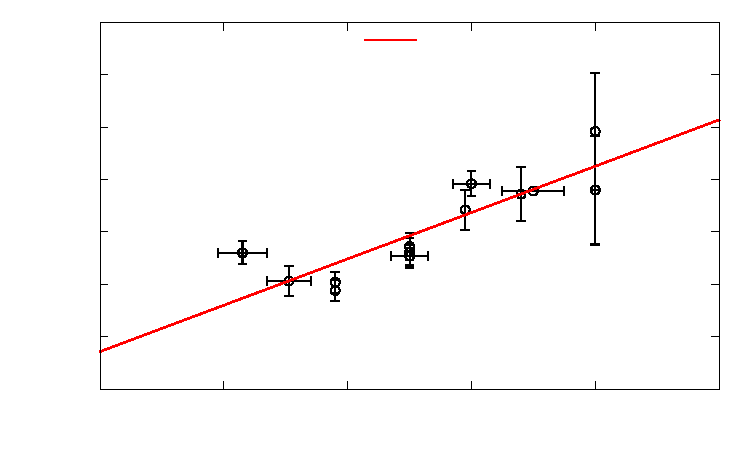
\includegraphics{GRAPH_Parameter_Fit_m-star_linear}}%
    \gplfronttext
  \end{picture}%
\endgroup

                        }\endgroup
                \caption{The evolution of $M^{*}$ as a function of redshift according to past observational studies.\label{fig:phi_evolution}}
            \end{figure}
        % subsubsection linear_parameter_evolution_with_redshift (end)
% subsection parameter_evolution (end)



    \section{Rate of Reionizing photons} % (fold)
\label{sec:rate_of_reionizing_photons}
	With a knowledge of the luminosity density, it is possible to calculate the star formation rate density, using the following formula.
	\begin{align}
		\rho_{SFR} &= 1\times 10^{-28}\rho_L
	\end{align}
	Using estimates of the fractional escape and zeta, we can use the formula above (7.7) to calculate the rate of reionization. From this, and the number of neutral hydrogen particles in the universe, it is possible to calculate the timescale of reionization.
	\begin{align}
	t =\frac{dNion}\d{t}\times \frac{1}{N_H}
	\end{align}
	Where t is the time between the start of reionization and the end, in seconds, Nion is the number of ionizing photons produced and $N_H$ is the number of Hydrogen atoms in the universe.

	As the number of photons produced roughly equalls the number of neutral hydrogen in the universe, it is possible to calculate a limit on the redshift accosiated with the end of reionization, given the corresponding opposite limit.

	A simulation of this was undergone using the equation above, and the resultant timescale was found to be\ldots

	\subsection{Techniques for Finding an Upper Limit on Redshift} % (fold)
	\label{sub:techniques_for_finding_an_upper_limit_on_redshift}
		We know that when $\rho_{SFR}$ and $\rho_{SFR}*$ are equal, reionization will begin. Knowing the Clumping factor (See Section X) it is possible to calculate the critical Star formation rate density, using the following equation,
		\begin{align}
		\rho_{SFR}*=2\times 10^3\frac{C}{f_{esc}} {\left( \frac{1+z}{10} \right )}^3
		\end{align}
		Where $f_{esc}$ is the fractional escape of photons from reionizing spheres, and C is the clumping factor. Combining with equation X it is possible to calculate the conditions for which reionization began as follows:
		\begin{align}
		1\times10^{-28}\int^{\infty}_{L}L\phi(L) dL=2\times 10^3\frac{C}{f_{esc}}{\left( \frac{1+z}{10} \right)}^3
		\end{align}
		Solving this equation, will give an upper z limit to reionization, and usign the timescale IN THE PREVIOUS SECTION it is possible to calculate both limits.

		The resultant values for redshift were z+/-z
	% subsection techniques_for_finding_an_upper_limit_on_redshift (end)

	\subsection{Jeans Mass for Collapse and Galaxy Formation} % (fold)
	\label{sub:jeans_mass_for_collapse_and_galaxy_formation}
		The Jeans Mass defines the cirtical mass of a cloud before it can collapse to form a galaxy, thereby limiting the minimum mass of a star foming galaxy. It is defined as the equation below:
		%\begin{align}
		%M_J=\left ( \frac{5kT}{Gm}\right ) ^{3/2} \left ( \frac{3}{4\pi\rho} \right ) ^{1/2}
		%\end{align}
		\begin{align}
		M_J = 5.73\times 10^3{\left(\frac{\Omega_mh}{0.15} \right)}^{-1/2} {\left( \frac{\Omega_b h^2}{0.022}\right)}^{-3/5} {\left( \frac {1+z}{10} \right)}^{3/2} M_\odot
		\end{align}
		Assuming an appropriate Mass-Luminosity ratio, this corresponds to an upper limit on both the Luminosity and the Absolute Magnitude (i.e.\ the dimmest ionizing galaxy.) This therefore provides a lower limit of magnitude to the schechter function, the L specified in the equation in the previous section

		\subsection{Mass-Luminosity Ratios}

		An appropriate Mass-Luminosity Formula is:
		\begin{align}
		L(M) = L_0 \times \frac {{(M/M_s)}^a} {q+{(M/M_s)}^{cd}}^{1/d}
		\end{align}
		where d=0.23, a=40 q=0.57 c=3.57\\
		\newline
		Or you can get the star formation rate of a galaxy from the mass (0911.1356v4) and from this you can obtain the Magnitude Kennicutt 1998 conversion from UV luminosity to AB magnitude and thereby to luminosity.
	% subsection jeans_mass_for_collapse_and_galaxy_formation (end)

	\subsection{Press Schechter Formalism} % (fold)
	\label{sub:press_schechter_formalism}
		PSF is a method of obtaining the number of objects with a specific mass within a certain volume. It assumes that the universe linearly ``clumped'' at the beginning of the universe, until a point where the density of the clumps break away from the rest of the universal expansion, and is treated as a massive body which collapses rapidly. (this occurs at around $\delta_c$\~1.68- Gunn and Gott). Press and Schechter suggest a probability distribution function of =:
		\begin{align}
		p(M,z)=-2p_0 \frac{\Delta P [\delta_v>\delta_c(z)]} {\Delta M} dM
		\end{align}
		Where $p_0$ is the mean density of the universe, and $\delta_c(z)$ is the overdensity threshold per redshift. P is the cumulative probability distribution of $\delta_v$ (volume)

		 It is from this that Schechter functions of luminosity and magnitude could arise\ldots
	% subsection press_schechter_formalism (end)

% section rate_of_reionizing_photons (end)

    %!TEX root = mainfile.tex

\section{Cosmic Variance} % (fold)
\label{sec:cosmic_variance}
	In general, the Universe can only be considered to be homogeneous at the most extreme distance scales ($>\SI{1}{\giga\parsec}$). At the scales which tend to be observed, matter in the Universe is not distributed uniformly and will gather together in massive clusters. Conversely, there will be empty regions of space, known as voids, where virtually no matter is present at all.

	Measurements deduced from observational surveys will certainly be affected by this large-scale cosmic structure. A measurement of an arbitrary region of the sky will have an associated uncertainty far greater than any sample variance due to Poisson statistics. This uncertainty is known as \emph{Cosmic Variance}, and will nearly always be the dominant source of error for any high-redshift cosmic survey. Given a probability distribution for the number counts, the cosmic variance is defined as:
	\begin{align}
		\sigma_v^2= \frac{\left \langle N^2 \right \rangle - \left \langle N \right \rangle^2}{\left \langle N \right \rangle}-\frac{1}{\left \langle N \right \rangle} \label{eq:cvstat}
	\end{align}
	where $\left \langle N \right \rangle$ is the mean and $\left \langle N^2 \right \rangle$ is the variance\cite{Trenti2008}.

	Any number or density measurement derived from a galaxy population is susceptible to cosmic variance. As an extreme example, it is reported to be potentially at the 50--70\% level in the HST UDF surveys\cite{Driver01102010}. Evidently, it will be particularly relevant to this study of cosmic re-ionization.

	\subsection{Factors which affect the Cosmic Variance} % (fold)
	\label{sub:factors_which_affect_the_cosmic_variance}
		Fortunately, there exist numerous ways of reducing the cosmic variance of a galaxy survey to a manageable amount, mostly accepted to be $<10\%$. As a general rule, this is achieved when a volume of \SI{e7}{\mega\parsec\cubed} is surveyed, with a square survey area over a single contiguous region\cite{Driver01102010}.

		The cosmic variance of a survey depends on three factors principally:
		\begin{itemize}
			\item it decreases steadily with volume
			\item it is reduced for higher aspect ratio surveys
			\item it is also reduced when multiple sight-lines are taken i.e.\ sparse sampling
		\end{itemize}
		Taking advantage of these factors, one can take steps to address the issue of cosmic variance.
	% subsection factors_which_affect_the_cosmic_variance (end)

		\subsubsection{Survey Volume} % (fold)
		\label{ssub:survey_volume}
			As mentioned above, the cosmic variance is heavily dependent on the volume of the survey, indicated by the steady decrease to lower percentages as larger volumes are surveyed, as in figure~\ref{fig:cv1}.  For volumes of \SI{e4}{\mega\parsec\cubed}, it is as much as 60\% whereas for \SI{e7}{\mega\parsec\cubed}, it will be 10\% and below.

			The dashed line below the main trend on the graph shows how the percentage uncertainty varies solely due to the sample variance. This gives some idea of the gulf between the effect of cosmic variance and that of Poisson statistics.
			\begin{figure}
				\centering
				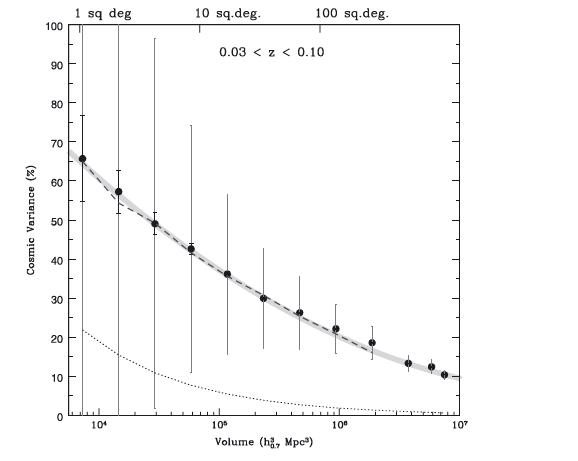
\includegraphics[width=0.7\textwidth]{../Images/cosmic_variance1.JPG}
				\caption{Graph showing the relation between the percentage cosmic variance and survey volume.\label{fig:cv1}}
			\end{figure}

			\begin{figure}
				\centering
				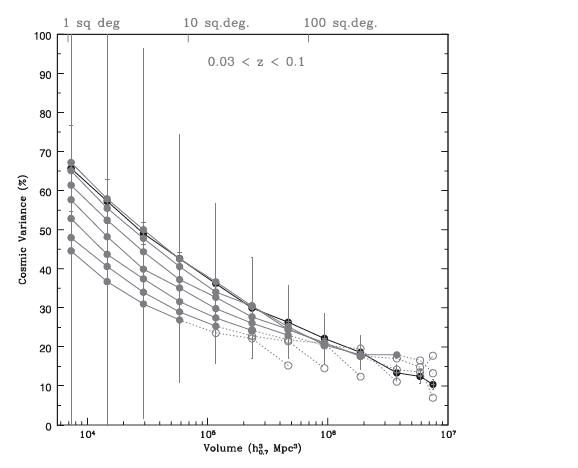
\includegraphics[width=0.7\textwidth]{../Images/cosmic_variance2.JPG}
				\caption{The same as for graph 1, this time with the additional grey points showing the dependence on aspect ratio. From the top to bottom they are 1:2, 1:4, 1:8, 1:16, 1:32, 1:64 and 1:128.}\label{fig:cv2}
			\end{figure}
		% subsubsection survey_volume (end)

		\subsubsection{Aspect Ratio} % (fold)
		\label{ssub:aspect_ratio}
			The aspect ratio of the survey is another crucial factor that can help deal with cosmic variance. For the same survey area, a long thin strip chosen over a standard square-shaped survey will decrease the cosmic variance. When taken to the extreme, this can cause a significant reduction. The same trend as for figure~\ref{fig:cv1} is shown in figure~\ref{fig:cv2}, but with the grey dots corresponding to higher aspect ratio surveys. The graph illustrates that, particularly for larger volumes, increasing the aspect ratio of a survey can make a huge reduction in the cosmic variance uncertainty.
		% subsubsection aspect_ratio (end)

		\subsubsection{Sparse Sampling} % (fold)
		\label{ssub:sparse_sampling}
			One might tackle cosmic variance in a very effective manner via the method of \emph{sparse sampling}, whereby several identical observing areas are distributed randomly across the sky. As opposed to one contiguous survey, these multiple sight-lines in different directions allow a more representative portion of the sky to be surveyed.

			It has been shown that cosmic variance is reduced with the number, $N$ of such sight-lines by $\frac{1}{\sqrt{N}}$. This holds irrespective of the base survey area\cite{Driver01102010}.
		% subsubsection sparse_sampling (end)

	\subsection{General Formula} % (fold)
	\label{sub:general_formula}
		In order to address cosmic variance in the code itself, an empirical formula was employed. In a paper (Driver and Robotham, 2010), this formula was derived using data from the SDSS (Sloan Digital Sky Survey), and extrapolated out to higher redshifts\cite{Driver01102010}. Due to its extrapolated nature, it should be noted that this is an approximate formula. Nonetheless, it should output a robust estimate of the cosmic variance for given surveys. Additionally, through it one can deduce possible ways to reduce the cosmic variance to below 10\%.
		\begin{align}
			\zeta _{CV}(\%)=\frac{\left( 1.00-0.03\sqrt{X-1} \right)\times \left( 219.7-52.4\log_{10}\left(291.0\times AB \right) + 3.21\log_{10}{\left(291.0\times AB\right)}^{2} \right)}{\sqrt{NC/291.0}} \label{eq:cvmain}
		\end{align}
		The formula employs the median redshift transverse lengths $A$ and $B$, and the radial depth $C$, all given in \si{\mega\parsec}, to represent the volume of each survey sample. The number of such samples i.e.\ the number of sight-lines is $N$. The aspect ratio is dealt with in the amplitude term at the front of the expression, where the aspect ratio 1:128 would be submitted as $X=128$, for example.

		Although it is extrapolated from an equation that applies at $z<0.1$, it takes advantage of the fact that cosmic variance should vary according to Poisson statistics along the radial length. This means that a survey with twice the radial depth will have $\sqrt{2}$ less cosmic variance. Hence the factor of $\sqrt{C}$ in the denominator. Equation~\ref{eq:cvmain} does not, however, make any corrections for the evolution of the clustering signature of the galaxy population, with this expected to be lower towards higher redshift. Correspondingly, any estimate output should be treated as an upper limit.

		This equation has been entered into the code which, from the survey parameters input, calculates the required quantities and gives an estimate of the cosmic variance as a percentage of the number counts expected to be observed. Furthermore, it will inform the user of how many random pointings of such a survey are necessary to achieve less than $10\%$ cosmic variance.
	% subsection general_formula (end)
% section cosmic_variance (end)

%written and researched by Lewis Clegg, coded by Andy King.

    %!TEX root = mainfile.tex

\section{Clumping Factor} % (fold)
\label{sec:clumping_factor}
(Lewis)

	hydrogen which already has been reionized may still play a significant role in the evolution of the Universe during the epoch of reionization, as it is still possible for it to recombine and become neutral once more. The average rate of recombinations is a significant factor which acts to slow down the expansion of the ionization front into the neutral inter-galactic medium. This rate, in turn, is proportional to a value known as the Clumping Factor. This factor is essentially a measure of the inhomogeneity in a medium, in this case, ionized hydrogen. In the what is known as the density field method, it is simply given by
	\begin{align}
		C_{DF} &=\frac{\left \langle n_\text{HII}^2 \right \rangle}{\left \langle n_\text{HII} \right \rangle^2}, \label{eq:clumpingnHII}
	\end{align}
	where $n_\text{HII}$ is the number density of ionized hydrogen in the inter-galactic medium, and $\left \langle n_\text{HII} \right \rangle$ is the average of this value\cite{2012ApJ...747..100S}.

	Many analytical and computational models are available which use the clumping factor to correct for recombinations during the reionization process. Some treat it as a global parameter, that is constant at all points in space. However, many believe a single value of the clumping factor will overestimate the recombination rate. Consequently, they choose to adopt a local parameter, which varies due to the density gradient of the inter-galactic medium. This also accounts for the negligible contribution of neutral gas to the recombination\cite{MNL2:MNL2993}.

	Other simulations generate a clumping factor which evolves over the period during which reionization took place. One such model (Iliev et al.~2007) has clumping evolving with redshift as\cite{Pawlik21042009},
	\begin{align}
		C &=26.2917\times \e{-0.1822z+0.003505z^2}. \label{eq:clumpingredshift}
	\end{align}
	For simplicity, in this project, the simpler method using a global variable was chosen. However, a redshift dependence scenario corresponding to that from equation~(\ref{eq:clumpingredshift}) was adopted, for better accuracy in the evolution of the critical star formation rate.
% section clumping_factor (end)

    %!TEX root = mainfile.tex

\section{Determining the rate of re-ionizing photons} % (fold)
\label{sec:determining_the_rate_of_re_ionizing_photons}
	When calculating the rate of re-ionizing photons, there are two important constants to be considered. These are the escape fraction of photons emitted by young stars which manage to escape from the galaxy, $f_\text{esc}$, and the number of hydrogen ionizing photons produced per second per unit star formation rate, $\zeta$. For the purposes of this project we will be using well established values nevertheless it is still important to understand how these values are obtained.

	\subsection{Escape Fraction} % (fold)
	\label{sub:escape_fraction}
		This value is the escape fraction of photons. If this number were one then every single photon that’s produced would escape from the galaxy into the IGM to contribute to the ionization of the neutral hydrogen however this is not the case. This figure is in fact much smaller meaning that most of the photons never reach the IGM at all. This is due to the neutral hydrogen within the galaxy itself absorbing the photons before they can escape. The amount of neutral hydrogen, the density and size of the galaxy and whether or not the galaxy is part of a cluster all contribute to the value of fesc and hence it is notoriously difficult to determine.

		It is often obtained by measuring the flux of UV photons below the Lyman limit of 912\AA which emerge from galaxies using methods such as intrepid spectroscopic and narrow-band imaging\cite{robertson2010early}. This is because only a certain fraction of the photons that were produced do emerge having managed to avoid interaction with the neutral gas within the galaxy thus measuring this flux directly and making assumptions of how many were initially produced would result in an estimate of the escape fraction. This comes with its own difficulties as often those photons which have managed to escape the galaxy are further absorbed by the IGM along the line of sight, reducing the flux that can be observed. As this method relies on observations it has not been possible to determine the escape value for high redshift galaxies and so it has been assumed that the number obtained from observations of lower redshift galaxies is approximately consistent at earlier cosmic times. As this value is so difficult to determine and varies from galaxy to galaxy it hasn’t been confirmed but instead has been constrained so hence this project will trial a range of these values to see how this can affect the rate of re-ionizing photons. Robertson et al.’s 2010 paper estimates this value to lie within the range $0.1\lesssim f_\text{esc}\lesssim 0.2$\cite{robertson2010early} whereas Inoue (2006) claims that ``fesc increases from a value less than 0.01 at $z\le1$ to about 0.1 at $z\ge 4$''\cite{inoue2006escape}. This contradicts the assumption that the escape fraction doesn’t alter with redshift however the approximate range of this value is what is required for this project not necessarily its evolution with time. Furthermore there isn’t enough data available to determine this to a great deal of accuracy and hence the extrapolated value for the escape fraction at high redshifts would be an approximation. As the value for the escape fraction can only vary from 0 to 1 its exact value cannot greatly alter the outcome of the calculation and thus an approximate value is sufficient within the realms of this project.

		The escape fraction can also be determined using galaxy formation simulations which is exactly what was done by Wood and Loeb in 2000. They found that the escape fraction at $z\approx 10$ is $\le1$\% for stars\cite{gnedin2008escape}. Calculating the escape fraction of ionizing photons from disk galaxies as a function of galaxy mass and redshift requires a complex code and that certain assumptions be made. These are that the gas in the disks is isothermal and radially exponential and that the source of radiation is either the stars within the disks or a central quasar. The mechanics of the program extend well beyond the scope of this project however the outcome of $f_\text{esc}=0.01$ is of use. As this particular paper was published in 2000 and has made relatively idealistic assumptions its legitimacy nowadays can be questioned. Therefore for the purposes of this project the observed values of $f_\text{esc}\approx 0.1$ have been used.
	% subsection escape_fraction (end)

	\subsection{Hydrogen Ionizing Photons Produced per Second per Unit Star Formation Rate} % (fold)
	\label{sub:hydrogen_ionizing_photons_produced_per_second_per_unit_star_formation_rate}
		The number of hydrogen ionizing photons produced per second per unit star formation rate is a very difficult number to pinpoint as it is not obvious how it could be determined numerically or observationally. This is because it is heavily dependent upon the characteristics of the star and, as each star is unique and stars themselves are so numerous, this becomes a very complex situation to simulate and thus it is common to take a representative average value for $\zeta$. Furthermore at the high redshifts considered in this project the stars are so far away that much bigger objects such as galaxies must instead be observed making it near-enough impossible to establish the activity of a single star.

		For the purposes of this project it has been assumed that $\zeta=10^{53.5}$\si{s^{-1}.M_{\odot}^{-1}.yr^{-1}}\cite{robertson2010early}. This particular value has been realised through the same detection methods as the escape fraction however as with fesc its precise value remains uncertain.

		The value for $\zeta$ can also be obtained numerically; more detail is included in Schull’s 2011 paper\cite{shull2012critical}. This applies a very complicated method however it essentially converts the star formation rate density into numbers of OB sequence stars and computes the total number of ionizing photons produced by a star of a certain mass over its lifetime. Combining this with the rate at which stars of this mass are formed would give a good estimate for $\zeta$. As this method is highly complex it is not clear to what extent it relates to the specifics of this project and hence although it is a highly advanced way of calculating $\zeta$ it is perhaps more sensible for the value obtained in Robertson to be used as this is a very common and better understood figure.
	% subsection hydrogen_ionizing_photons_produced_per_second_per_unit_star_formation_rate (end)
% section determining_the_rate_of_re_ionizing_photons (end)

% part predictions (end)
\newpage
\part{Observations} % (fold)
\label{prt:observations}
    %!TEX root = mainfile.tex
\section{Observing Strategy Group} % (fold)
\label{sec:observing_strategy_group}
	This primary aim of this subgroup is to formulate an observing strategy capable of probing the depths of the Epoch of Re-ionization. Our strategy is going to be based upon using optical techniques to detect candidate Lyman Break Galaxies (LBG) and confirming their properties using spectroscopy.

	The study of this era in the universe’s history has come a long way in the past 30 years and with the selection of new telescopes and radio arrays being designed currently it is only set to accelerate over the coming decades. It is a massive understatement to say such distant redshifts are very difficult to see and it is a testament to scientific and engineering achievement that we are able to take the detailed images we can. The light from these galaxies is so faint that it can take a very long time to see anything. Due to this lengthy nature of the projects, time on telescopes is highly sought after and very competitive.

	This strategy must therefore be as complete as possible with as many influencing factors included. This strategy will have two main focuses:
	\begin{itemize}
		\item Using the most efficient methods available in order to limit the observing time required.
		\item To probe the beginning of re-ionization; there have been few observations above $z=10$ and future telescopes will have the ability to break new frontiers and observe what happened at these earliest moments of structure formation.
	\end{itemize}

	Our strategy will look to utilise the capabilities of the new technology to further the scientific understanding of the EoR.

	The observing strategy will be established as follows:
	\begin{itemize}
		\item Research possible telescopes capable of observing high-redshift objects.
		\item Explore the advantages and disadvantages of ground and space-based telescopes.
		\item Identify the most efficient telescope for a wide survey of the sky to locate candidates; this will be determined using exposure time calculations.
		\item Research gravitational lensing, its possible application in assisting our wide surveys and how we might locate more lenses.
		\item Identify the telescope which will produce the highest resolution imaging of in a narrower deep survey; this will be established using exposure time calculations and observational limits of the system.
		\item Identify a telescope capable of spectroscopically confirming the nature and redshift of the candidates.
		\item Investigate the application of methods such as colour-colour diagrams for selecting candidates and removing contaminants from the sample.
		\item Compile a ‘Final Observing Strategy’ capable of observing the EoR using numerical predictions from the predictions subgroup.
	\end{itemize}
	This `Final Observing Strategy' will give calculations of the observation time required (inc.\ photometry, overheads, spectroscopy), the timescale on which the project can be actioned, the limitations of our strategy, possible areas for optimisation/refinement and areas for further research.

% section observing_strategy_group (end)

    %!TEX root = mainfile.tex

\section{Determining Redshift} % (fold)
\label{sub:determingin_redshift}
	Need a section on candidates and how the contaminants are eliminated.
	(COMBINE WITH JOE'S COLOUR STUFF?)

	Section~\ref{sec:contaminants} described how contaminants could be eliminated from the large number of potential high redshift galaxies. Taking the remaining objects, the following methods are used to check whether they are in fact LBGs.

	\subsection{Filters and the Dropout Technique} % (fold)
		\label{ssub:filters_and_the_dropout_technique}
		Using photometry, the redshift of a LBG can be estimated using the dropout technique: The flux from the galaxy can be measured in three different bands, ideally two above and one below the Lyman break. If the galaxy is a high redshift Lyman break galaxy, it would be expected that, so long as the filters were correct for the redshift expected, one image would not see the galaxy whereas the other two would observe flux. Below in figure~\ref{fig:drop_out_at_z7}, the dropout technique is shown for a model galaxy of redshift seven.
		\begin{figure}[!htb]
			\centering
			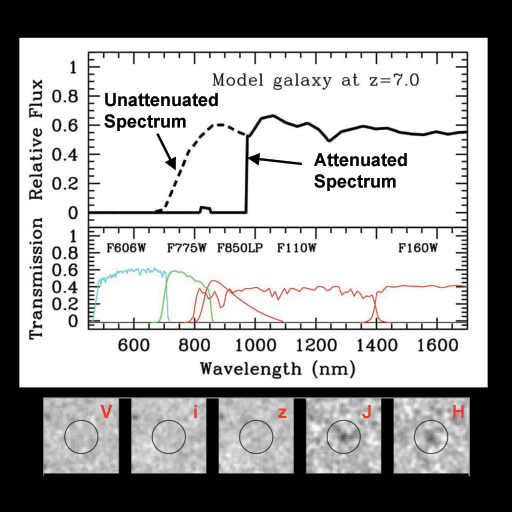
\includegraphics[width=0.5\textwidth]{../Images/drop_out_at_z7.png}
			\caption{Dropout technique for model redshift 7 galaxy\cite{first_galaxies_dropout_at_z7}.\label{fig:drop_out_at_z7}}
		\end{figure}

		The neutral hydrogen has attenuated almost all flux at wavelengths shorter than approximately 1 micrometre. The galaxy has been imaged in several different bands, and the longer wavelength filters show flux, whereas those at wavelengths corresponding to blue-ward of Lyman alpha do not. The galaxies that the group look to study have been shifted such that the drop happens in the infrared. The wavelength of the drop can be worked out using the known rest wavelength of Lyman alpha, as well as the factor by which the wavelength shifts due to the expansion of the universe, as shown in equation~\ref{eq:dropout_wavelength}.
		\begin{align}
			\text{Rest wavelength of Lyman alpha} \times (1+z) &= \text{observed wavelength of drop}\label{eq:dropout_wavelength}
		\end{align}

		Since the rest wavelength of Lyman alpha is known and the observed wavelength of the drop can be measured, the redshift of the galaxy can be determined. This
		is only a rough estimate when doing photometry since the flux is simply a number in each of the bands. For example, if the bands do not overlap, and the drop happens between two bands, it will not be known at what point the drop occurred, only the range in which it occurred. This motivates the use of bands which are close together or potentially even overlapping. Figure~\ref{fig:filter-systems} shows some different bands and their bandwidth, for different filter systems. Johnson-Cousins- Glass is one of the oldest and still the most commonly used system\cite{BasicObservationalKnowledge}.
		\begin{figure}[!htb]
			\centering
			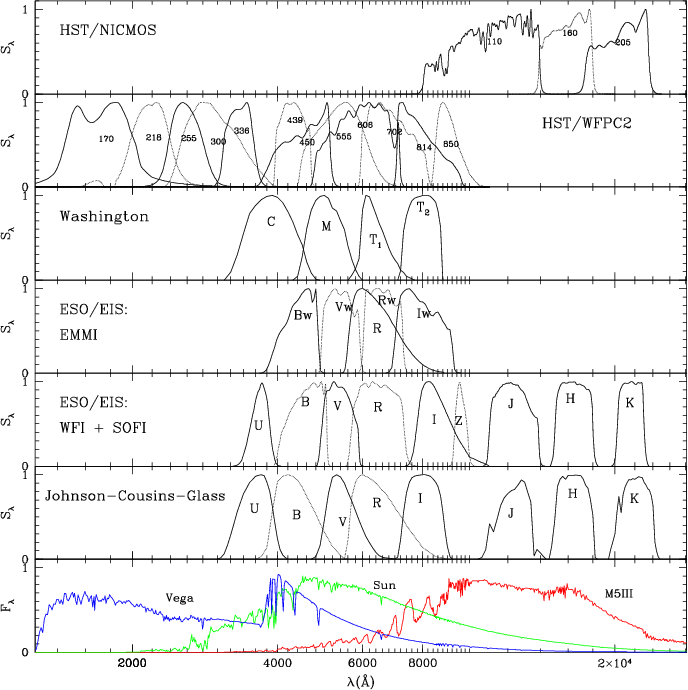
\includegraphics[width=0.65\textwidth]{../Images/filter-systems.png}
			\caption{Various filtering systems\cite{refId0}.\label{fig:filter-systems}}
		\end{figure}

		The bandwidth (or passband) is the wavelength range that can pass through the filter. Filters in different parts of the spectrum are given a common name, for example I band at \SI{806}{\nano\metre}. When observing LBGs, it is beneficial to have three filters in a row so that the position of the drop can be more accurately measured. As can be seen, there are gaps between the J H and K filters, meaning if the drop occurs between J and H, full flux should be observed in H and K and virtually no flux should be seen in J. (the panels beneath figure~\ref{fig:filter-systems} show an image (or lack thereof) of the $z=7$ galaxy in each of the V, I, z, J and H bands)

		Table~\ref{tab:filter_characteristics} below shows a list of filter names, the central wavelength of that filter, the bandwidth the filter covers, and range of redshifts for which the Lyman alpha drop would be covered. (This  range assumes the bandwidth covers 50\% either side of the central wavelength)
		\begin{table}[ht]
			\begin{center}
				\begin{tabular}{c|c|c|c}
					Filter 	& Central wavelength & Bandwidth & Redshift coverage \\
					\hline \hline
					V 	& \SI{551}{\nano\metre}	 & \SI{88}{\nano\metre} & 3.17--3.90 \\
					i 	& \SI{806}{\nano\metre}	 & \SI{149}{\nano\metre} & 5.01--7.25 \\
					Y 	& \SI{1020}{\nano\metre} & \SI{120}{\nano\metre} & 6.90--7.88 \\
					J 	& \SI{1220}{\nano\metre} & \SI{213}{\nano\metre} & 9.16--9.91 \\
					H 	& \SI{1630}{\nano\metre} & \SI{307}{\nano\metre} & 11.14--13.67 \\
					K 	& \SI{2190}{\nano\metre} & \SI{390}{\nano\metre} & 15.41--18.61
				\end{tabular}
			\end{center}
			\caption{Data highlighting which filters would be useful for observing particular redshift galaxies\cite{Galactic_Astronomy_Binney_Merrifield}}
			\label{tab:filter_characteristics}
		\end{table}

		Table~\ref{tab:filter_characteristics} must be taken into consideration that two filters should be red-ward of the drop and one blue-ward. One the fluxes have been measured in all three bands, if the object is indeed a LBG, there should be a sharp drop in flux in  one of the bands. However this does not totally rule out other possibilities: Some other objects could also exhibit a drop in flux, posing as LBGs, so usually a follow up method is used, and this is spectroscopy. Spectroscopy The drop out technique provides a good indication that a galaxy is a high redshift Lyman break galaxy, however the best way to confirm this is with spectroscopy. Spectroscopy involves\ldots

		At loads of different wavelengths, measure the spectra. Look for the drop

		Use ground based such as KECK or space based, JWST will have one.

		%JOHN IS DOING SPECTROSCOPY. I AM NOT NEEDED HERE.
		% subsection filters_and_the_dropout_technique (end)

% subsection determining_redshift (end)

    %!TEX root = mainfile.tex

\section{Photometry and Colour} % (fold)
\label{sec:Photometry_Colour}
	Photometry today is used primaily with CCDs, which can convert the transmitted flux into an electric signal which can then be interpretted as a magnitude. The magnitude system used in this project was the AB magnitude system as outlined in Section~\ref{ssub:ab_magnitude}.

	In this project wide and intermediate filters have been used predominantly. A common method for making these filters is to use coloured glass which either pass all light above a certain wavelength or pass all light up to a certain wavelength, these are known as cutoff filters. A bandpass filter can be made by combining two types of coloured glass, one which will act as the low wavelength cutoff and the other as the high wavelength cutoff. Filters don't transmit 100\% of the wavelengths that are allowed to pass, and the cutoff isn't at an exact frequency.

	To detect lyman-break galaxies the dropout method is used, which uses at least three filters to get enough spectral information to identify the object as a candidate for being a lyman break galaxy (see dropout method Section~\ref{ssub:dropout_technique}). However, observing the drop due to the Gunn-Peterson effect is not enough to confirm the identities of these candidates, other observational methods need to be used to be certain the object is a lyman break galaxy and not a contaminant. One of the most effective ways of eliminating contaminants is to use the colour of the object between different filters, obtained from the photometric measurements. The filters for each telescope were decided by determining where the lyman-break wavelength would appear at a certain redshift, using the equation,
	\begin{align}
		z=\frac{{{\lambda}_\text{obs}}-{{\lambda}_\text{emit}}}{{{\lambda}_\text{emit}}}
	\end{align}
	and finding which filter would contain this wavelength. The two filters either side of this filter were chosen as well for colour observations and for the dropout technique. The table below shows the filters used for various red shift ranges, with the filter in the middle of each redshift range being the filter where the lyman break would be observed. Note that the James Webb telescope and Euclid are the only telescopes shown because they were the telescopes chosen for the strategy.
	\begin{table}[ht]
		\centering
			\begin{tabular}{c|c|c}
				Redshift range &Telescope &Filters   \\
				\hline \hline
				6-7.5	   &James-Webb&  F070w, F090w, F115w \\
				7.5-8.5&James-Webb&  F090w, F115w, F150w \\
				8.5-10 &Euclid&  Y, J, H\\
				10-14  &James-Webb& F115w, F150w, F200w\\
				14-15  &0.105& F150w, F200w, F277w\\
			\end{tabular}
		\caption{Table showing filters used for different redshift ranges}
		\label{tab:colour_filters}
	\end{table}.


    \subsection{Contaminants} %fold
    \label{sub:Contanimants}
    	\subsubsection{Sources of Contamination} % (fold)
    	\label{ssub:sources_of_contamination}
    	%Need to be one level lower, may change

		    \subsubsection*{Low Mass Stars} % (fold)
		    \label{sub:low_mass_stars}
		        These can easily be identified due to the high resolution imaging provided by JWST and Euclid. The Point-spread function (PSF) obtained will allow us to determine which sources are point-like and which are extended. We should be able to avoid significant contamination by removing any point-like sources from the results as all galaxies should have a great enough diameter.
		    % subsection low_mass_stars (end)

		    \subsubsection*{Spurious Sources} % (fold)
		    \label{sub:spurious_sources}
		        By stipulating that we will be requiring detections in two bands the influence of spurious sources will be negligible. Finding detections in 2/3 bands at reasonable confidence interval ($S/N =5$) is very improbable. By inspecting the negative with the same requirements for detection we are able to easily identify any such sources.\cite{Bouwens2011}.
		    % subsection spurious_sources (end)

		    \subsubsection*{Supernovae and other transient sources} % (fold)
		    \label{sub:supernovae_and_other_transient_sources}
		        Events such as Supernovae happen incredibly quickly releasing a vast amount of energy, as seen in Figure~\ref{fig:SNe_1987a}. These events can spoil images due to their short duration by introducing new data in only a portion of the sample. These effects are usually only considered when taking exposures years apart or when combining multiple sources over a long time scale. Such events are very unlikely to contaminate our results as we propose to take our images close in time.
		        \begin{figure}[htbp]
		            \centering
		            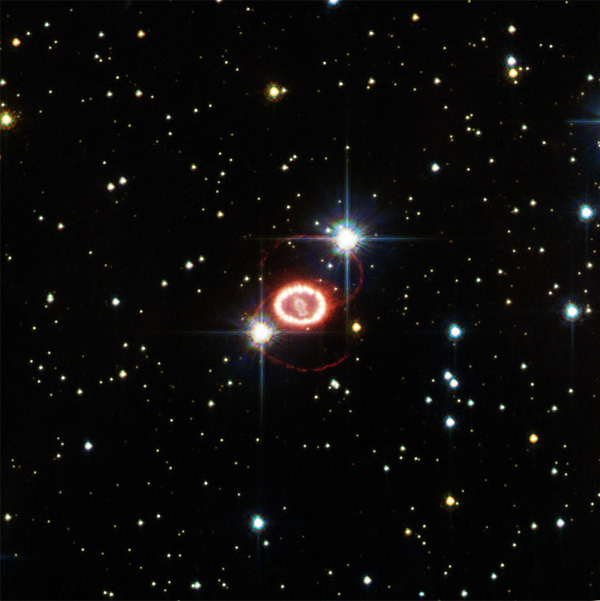
\includegraphics[width=0.6\textwidth]{../Images/SNe_1987a.jpg}
		            \caption{The shock wave from Supernova 1987a imaged by HST in 2006.\label{fig:SNe_1987a}}
		        \end{figure}
   			 % subsection supernovae_and_other_transient_sources (end)

		    \subsubsection*{Lower Redshift Sources and photometric scattering} % (fold)
		    \label{sub:lower_redshift_sources_and_photometric_scattering}
		        This category is likely to provide the greatest source of contamination for the surveyed area. It will do so increasingly at high redshifts where its affect on the faintest magnitudes is most greatly felt. Its affect is most influential with a small S/N ratio for the observations, by fixing this at a level of $S/N = 5$ we can be confident that the contamination will be low. Detecting a source in another band such as b435, v606, i775 for YJH photometry would class it as a contaminant and then should be removed from sample, however we wont use this as it would too greatly increase the time.
		    % subsection lower_redshift_sources_and_photometric_scattering (end)

    	% subsubsection sources_of_contamination (end)
    	\subsubsection{Eliminatiing Contaminants} % (fold)
    	\label{sub:eliminatiing_contaminants}
			The \emph{colour} of an object in photometry is defined as the difference in magnitude between two filters\cite{Romanishin}. If there are two filters, for example purposes let them be called A and B, where A has a lower central wavelength, the colour for an object in these two filters would be,
			\begin{align}
				m_A-m_B=-2.5\log\left(\frac{f_A}{f_B}\right).
			\end{align}
			where $f_A$ and $f_B$ are the specific flux denisites of the filters A and B\cite{Romanishin}. The colour is therefore equivalent to the ratio of specific flux densities, this means two objects with the same colour can have different magnitudes in each of the filters. If the colour is positive it is said to be `red' and if it is negative it is said to be `blue', i.e. an an object which is red between two filters has a lower flux in the blueward filter compared to the redward filter and an object which is red has a larger flux in the blueward filter than the redward one.  The larger the value is, it is said that the `redder' the object is. To eliminate contaminants from observations, a colour-colour diagram can be made using three filters, with two colour values for each object. For instance if the observations were done in the J, H and K filters, the colour colour diagram would be (H-K) plotted against (J-H). Although this study does not take any observtions, colour diagrams can be built up for observations by simulating a catalog of lyman break galaxies at high redshift and determine colour windows for observations using the program Hyperz. Lyman-break galaxies are very red in colour for the filter blueward of the break and over the break due to the extreme drop in flux blueward of the lyman-break, and they will be a low red value or even blue value for the colour between the filter over the break and redward of the break, due to the decrease in flux past the break. In this way contaminants as described in Section~\ref{sec:contaminants} can be removed quickly from observations.
    	% subsection eliminatiing_contaminants (end)
	%subsection Eliminating_Contaminants (end)
% section contaminants (end)

    \subsection{Hyperz} %fold
	\label{sub:Hyperz}
		To eliminate contaminates and predict colour windows for observations the program Hyperz and its subprogram `make\_catalog' can be used to produce a catalog of synthetic galaxies and their magnitudes in different filters at different redshifts.

        \subsubsection{Inputs} %fold
        \label{subsub:Hyperz_inputs}
			To produce this catalog, a set of inputs are put into the catalog file. The operation of the program is quite complex and is only summarised here. Also, the operation of make catalog is slightly different to Hyperz and a full manual for make catalog was not obtainable. The program starts with a sample Spectral Energy Distribution (SED), which has key features such as the lyman-break which will appear as the redshift is increased, the program combines this with a sample burst spectrum, which assumes the stars formed quickly, which is a good assumption for high redshift galaxies\cite{hyperz}. The Predictions group schecter function used the \SI{1500}{\angstrom} rest UV wavelength with the assumption that the flux from a lyman break galaxy was approximately the same for \SI{1350}{\angstrom} to \SI{1750}{\angstrom}. The program uses a known magnitude in a reference filter to fit the SED and to find the magnitde of the object in other bands. Using the Prediction's group program, a range of magnitudes can be found for a certain redshift interval by looking at the number of galaxies for a certain magnitude at a certain redshift. As the redshifted \SI{1500}{\angstrom} line will move with redshift, a range of reference filters were required to cover the redshift range for the observing strategy. As the flux is assumed to be constant over the range \SI{1350}{\angstrom}--\SI{1750}{\angstrom}, this meant a single filter could be used for a wide interval of redshifts. The reference filters were chosen to have a central wavelength as close to the central \SI{1500}{\angstrom} wavelength for that redshift. The reference magnitudes were based upon the predictions program for calculating the number density of galaxies. For each redshift range a lower magnitude was chosen based on whether any galaxies were observed below the chosen magnitude. The maximum magnitude was chosen to 35, as this was the limit the observing strategy had chosen to use. The reference magnitude ranges are therefore different sizes, and this is perhaps not wise to be able to compare similar redshifts, further consideration of reference magnitudes would have been desirable. Below is a table listing the reference filters used. Note that filter 44 was not correctly labelled in the database of filters! This created unforseen problems for the Euclid magnitudes and it wasn't apparant for a long time that the reference filter was to blame.
			\begin{table}[ht]
				\begin{center}
					\begin{tabular}{c|c|c}
						Redshift range & reference filter number&reference magnitudes \\
						\hline \hline
						6-7.5	   &34&27-35\\
						7.5-8.5&55&27.5-35\\
						8.5-10 &44&28-35\\
						10-14  &35&29-35\\
						14-15  &72&30-35\\
					\end{tabular}
				\end{center}
				\caption{Table showing reference filters and magnitudes used}
				\label{tab:reference_filters}
			\end{table}.

			There are several other inputs which are easy to understand: the user chooses the range of redshifts for the catalog, the formation redshift, which is when the galaxies started forming and to keep consistency between the two groups, the same cosmological constants were used as the predicitons group, which were: $\Omega_M=0.27$, $\Omega_\Lambda=0.73$ and $H_0=\SI{71}{\kilo\metre\per\second\per\mega\parsec}$. Two other parameters which are slightly more complex are the age of the galaxies and the reddening law. To simplify the calculations, the age of the galaxies was set such that galaxies at the same redshift have the same age, forming at the same moment at the formation reshift. The other choice for the galaxies to be born somewhere randomly between the formation redshift and the observed redshift. The reddening law is a more detailed input and is considered below.
		%subsubsection Inputs (end)

		\subsubsection{Reddening Law} % (fold)
		\label{ssub:reddening_law}
			Hyperz can account for Reddening of galaxies. Reddening refers to the SED of a galaxy appearing redder than it actually is and is one of the effects due to the prescence of dust. Dust is matter within galaxies that inteferes with the photons travelling towards the observer. Through spectral analysis, it has been determined that dust is composed of substances such as Carbon, silicate materials, water and ammonia in the form of ice amongst other substances \cite{stein1983dust}. Dust can absorb (and emit) photons, with absorbtion occuring most in the UV and therefore the spectrum appears reddened\cite{stein1983dust}. Hyperz allows the user to select one of five laws to apply to the catalogs produced, and the law that was chosen for the purposes of this study was the Calzetti et al. (2000). There were two reasons for this: it seems to be the law that most recent papers use and appears to be a more general approximation than other laws which are based on specific galaxies and it is a law for starburst galaxies, which corresponds to the sample spectrum used. The program asks for a maximum and minimum value of extinction in terms of magnitude, defined as $A_V$. Several steps are required to get to this required value. Starting with the equation
			\begin{align}
				A_\lambda=k(\lambda)E(B-V)=\frac{k(\lambda)A_V}{R_V}
			\end{align}
			where $A_\lambda$ is defined as the extinction at a certain wavelength, $k(\lambda)$ is the reddening curve, E(B-V) is the colour excess and $R_V$ is a constant \cite{hyperz}. The equation can be arranged to find $A_V$,
			\begin{align}
				A_V=\frac{k(\lambda)A_\lambda}{R_V}.
			\end{align}
			$R_V$ is given as $4.05 {\pm} 0.8$ \cite{hyperz} for the Calzetti law and
			\begin{align}
				k(\lambda)=2.659(-1.857+\frac{1.040}{\lambda})+R_V
			\end{align}
			for $0.12{\mu}m \le \lambda \le 0.63{\mu}m$ for the Calzetti law\cite{hyperz}. $\lambda$ is assumed to be the emitted wavelength from the galaxy, which will be assumed to be 1216$\angstrom$ as an assumption to simplify the calculation. The only unknown is $A_\lambda$. From the equation
            \begin{align}
				f_{obs}(\lambda)=f_{int}(\lambda)10^{-0.4A_\lambda}
			\end{align}
			where $f_{obs}$ is the observed flux and $f_{int}$ is the intrinsic flux, which is the flux if no reddening occured\cite{hyperz}. It can be seen that if $A_\lambda=0$ then there is no reddening, which leads to a value of zero for $A_V$. This can then be set for the minimum value for the Reddening law, although it will be very improabable for there to be no extinction, it is theoretically possibly and simplifies the situation. the maximum value for $A_V$ is harder to find as this project doesn't take any observations and the program from the predictions group gives intrinsic fluxes, so values were found using NED's Coordinate and Galactic Extinction Calculator\cite{NEDex}. Using a set of galaxies from various papers in a redshift range of 6--9, their Right Ascension and Declination were inputted into the calculator, which then found values of $A_\lambda$ for a range of filters. For each redshift the filter chosen contained the redshifted lyman break for those galaxies, the galaxy with the maximum extinction value was chosen for each redshift range. In the table below are the values obtained. For redshift 10--15 the data was extrapolated to find values. The maximum difference in $A_\lambda$ between redshifts was found for the known galaxies, and then this was applied for each increase in redshift.
			\begin{table}[ht]
				\begin{center}
					\begin{tabular}{c|c|c}
						Redshift range & $A_\lambda$ & $A_V$  \\
						\hline \hline
						6-7.5	   &0.013&  0.0044 \\
						7.5-8.5&0.013&  0.0044 \\
						8.5-10 &0.036&  0.0122\\
						10-14  &0.082&  0.0277\\
						14-15  &0.105&  0.0355\\
					\end{tabular}
				\end{center}
				\caption{Table showing values of Extinction for different redshift values}
				\label{tab:extinction_values}
			\end{table}.

			These values were put into the catalog. Many assumptions were made to find this value, so it may be incorrect. Articles tend to have a much bigger value for the maximum extinction, for example in the Hyperz manual it is 1.2. However the best possible figure was obtained with the resources avalaible. the extinction due to the Milky Way has not been considered which might have made a significant difference.
		% subsubsection reddening_law (end)

		\subsubsection{Vega to AB Conversions} % (fold)
		\label{ssub:vega_to_ab_conversions}
			Hyperz works in Vega magnitudes so AB conversions are needed. These conversions are complex and therefore conversions for a ground based telescope for typical filters have been used from\cite{Graham} Filters were compared to the nearest equivalent but some will inevitably be different from the actual values. The reference filters were from the database of filters that came with Hyperz and so came ready with conversions to AB. The conversions for the reference filters were applied for the input into the program, and the output magnitude in the various filters were changed to AB from Vega. The table below shows the conversion for each filter chosen for observation.
			\begin{table}[ht]
				\begin{center}
					\begin{tabular}{c|c}
						Filters & M(AB)-M(Vega) \\
						\hline \hline
						F070w, F090w,  & 0.5 \\
						F115w, Euclid Y, Euclid J	& 0.9\\
						 F150w, Euclid H	& 1.4\\
						F200w, F275w & 1.9\\
					\end{tabular}
				\end{center}
				\caption{AB conversions for filters}
				\label{tab:AB_conversion}
			\end{table}
		% subsubsection vega_to_ab_conversions (end)

		\subsubsection{Output} % (fold)
		\label{ssub:output}
			After running the executable file, the output is shown in a catalog, each redshift calaculated is random, so the galaxies are in a random order. From the output, the colour of an object can be found after the AB conversions have been made to the magnitudes and a colour diagram can then be plotted.
		% subsubsection output (end)
	%subsection Hyperz (end)

	\subsection{Results for Colour} %fold
	\label{sub:Results_for_Colour}
		Below are the results for four of the specified ranges, the redshift range 14 to 15 was not included here as there was an unresolved problem with the F275w filter on NIRcam, which will be discussed below. The colour windows were found by finding the minimum value of the y-axis and the maximum value of the x-axis and stating that the colour window must be greater than or equal to and less than or equal to the values on the axes respectively, isolating the upper left quadrant of each colour diagram to be the colour window.
		\begin{figure}[htbp]
			\begin{minipage}[c]{0.5\linewidth}
				\centering
					\begingroup\endlinechar=-1
						\resizebox{\textwidth}{!}{%
							% GNUPLOT: LaTeX picture with Postscript
\begingroup
  \makeatletter
  \providecommand\color[2][]{%
    \GenericError{(gnuplot) \space\space\space\@spaces}{%
      Package color not loaded in conjunction with
      terminal option `colourtext'%
    }{See the gnuplot documentation for explanation.%
    }{Either use 'blacktext' in gnuplot or load the package
      color.sty in LaTeX.}%
    \renewcommand\color[2][]{}%
  }%
  \providecommand\includegraphics[2][]{%
    \GenericError{(gnuplot) \space\space\space\@spaces}{%
      Package graphicx or graphics not loaded%
    }{See the gnuplot documentation for explanation.%
    }{The gnuplot epslatex terminal needs graphicx.sty or graphics.sty.}%
    \renewcommand\includegraphics[2][]{}%
  }%
  \providecommand\rotatebox[2]{#2}%
  \@ifundefined{ifGPcolor}{%
    \newif\ifGPcolor
    \GPcolortrue
  }{}%
  \@ifundefined{ifGPblacktext}{%
    \newif\ifGPblacktext
    \GPblacktexttrue
  }{}%
  % define a \g@addto@macro without @ in the name:
  \let\gplgaddtomacro\g@addto@macro
  % define empty templates for all commands taking text:
  \gdef\gplbacktext{}%
  \gdef\gplfronttext{}%
  \makeatother
  \ifGPblacktext
    % no textcolor at all
    \def\colorrgb#1{}%
    \def\colorgray#1{}%
  \else
    % gray or color?
    \ifGPcolor
      \def\colorrgb#1{\color[rgb]{#1}}%
      \def\colorgray#1{\color[gray]{#1}}%
      \expandafter\def\csname LTw\endcsname{\color{white}}%
      \expandafter\def\csname LTb\endcsname{\color{black}}%
      \expandafter\def\csname LTa\endcsname{\color{black}}%
      \expandafter\def\csname LT0\endcsname{\color[rgb]{1,0,0}}%
      \expandafter\def\csname LT1\endcsname{\color[rgb]{0,1,0}}%
      \expandafter\def\csname LT2\endcsname{\color[rgb]{0,0,1}}%
      \expandafter\def\csname LT3\endcsname{\color[rgb]{1,0,1}}%
      \expandafter\def\csname LT4\endcsname{\color[rgb]{0,1,1}}%
      \expandafter\def\csname LT5\endcsname{\color[rgb]{1,1,0}}%
      \expandafter\def\csname LT6\endcsname{\color[rgb]{0,0,0}}%
      \expandafter\def\csname LT7\endcsname{\color[rgb]{1,0.3,0}}%
      \expandafter\def\csname LT8\endcsname{\color[rgb]{0.5,0.5,0.5}}%
    \else
      % gray
      \def\colorrgb#1{\color{black}}%
      \def\colorgray#1{\color[gray]{#1}}%
      \expandafter\def\csname LTw\endcsname{\color{white}}%
      \expandafter\def\csname LTb\endcsname{\color{black}}%
      \expandafter\def\csname LTa\endcsname{\color{black}}%
      \expandafter\def\csname LT0\endcsname{\color{black}}%
      \expandafter\def\csname LT1\endcsname{\color{black}}%
      \expandafter\def\csname LT2\endcsname{\color{black}}%
      \expandafter\def\csname LT3\endcsname{\color{black}}%
      \expandafter\def\csname LT4\endcsname{\color{black}}%
      \expandafter\def\csname LT5\endcsname{\color{black}}%
      \expandafter\def\csname LT6\endcsname{\color{black}}%
      \expandafter\def\csname LT7\endcsname{\color{black}}%
      \expandafter\def\csname LT8\endcsname{\color{black}}%
    \fi
  \fi
  \setlength{\unitlength}{0.0500bp}%
  \begin{picture}(7200.00,4320.00)%
    \gplgaddtomacro\gplbacktext{%
      \put(747,595){\makebox(0,0)[r]{\strut{} 3}}%
      \put(747,1047){\makebox(0,0)[r]{\strut{} 3.5}}%
      \put(747,1500){\makebox(0,0)[r]{\strut{} 4}}%
      \put(747,1952){\makebox(0,0)[r]{\strut{} 4.5}}%
      \put(747,2404){\makebox(0,0)[r]{\strut{} 5}}%
      \put(747,2856){\makebox(0,0)[r]{\strut{} 5.5}}%
      \put(747,3309){\makebox(0,0)[r]{\strut{} 6}}%
      \put(747,3761){\makebox(0,0)[r]{\strut{} 6.5}}%
      \put(849,409){\makebox(0,0){\strut{} 3.5}}%
      \put(1453,409){\makebox(0,0){\strut{} 4}}%
      \put(2058,409){\makebox(0,0){\strut{} 4.5}}%
      \put(2662,409){\makebox(0,0){\strut{} 5}}%
      \put(3267,409){\makebox(0,0){\strut{} 5.5}}%
      \put(3871,409){\makebox(0,0){\strut{} 6}}%
      \put(4475,409){\makebox(0,0){\strut{} 6.5}}%
      \put(5080,409){\makebox(0,0){\strut{} 7}}%
      \put(5684,409){\makebox(0,0){\strut{} 7.5}}%
      \put(6289,409){\makebox(0,0){\strut{} 8}}%
      \put(6893,409){\makebox(0,0){\strut{} 8.5}}%
      \csname LTb\endcsname%
      \put(144,2178){\rotatebox{-270}{\makebox(0,0){\strut{}f070w-f090w}}}%
      \csname LTb\endcsname%
      \put(3871,130){\makebox(0,0){\strut{}f090w-f115w}}%
      \put(3871,4040){\makebox(0,0){\strut{}Redshift 6--7.5}}%
    }%
    \gplgaddtomacro\gplfronttext{%
    }%
    \gplbacktext
    \put(0,0){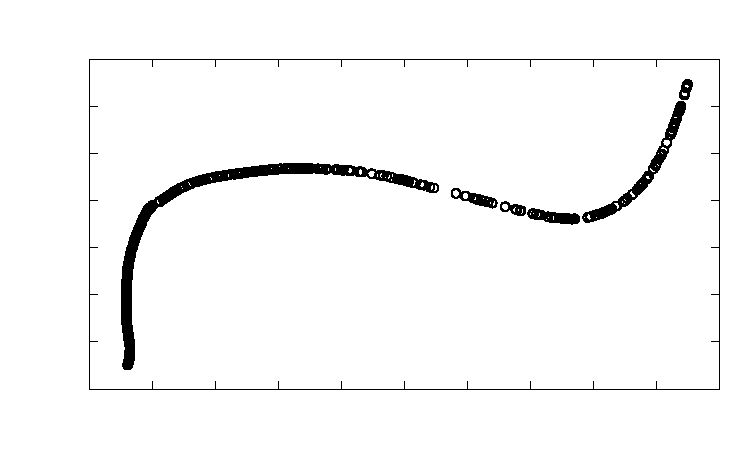
\includegraphics{GRAPH_color_graph1}}%
    \gplfronttext
  \end{picture}%
\endgroup

						}\endgroup
				\caption{A\label{fig:col1}}
			\end{minipage}
			\begin{minipage}[c]{0.5\linewidth}
				\centering
					\begingroup\endlinechar=-1
						\resizebox{\textwidth}{!}{%
							% GNUPLOT: LaTeX picture with Postscript
\begingroup
  \makeatletter
  \providecommand\color[2][]{%
    \GenericError{(gnuplot) \space\space\space\@spaces}{%
      Package color not loaded in conjunction with
      terminal option `colourtext'%
    }{See the gnuplot documentation for explanation.%
    }{Either use 'blacktext' in gnuplot or load the package
      color.sty in LaTeX.}%
    \renewcommand\color[2][]{}%
  }%
  \providecommand\includegraphics[2][]{%
    \GenericError{(gnuplot) \space\space\space\@spaces}{%
      Package graphicx or graphics not loaded%
    }{See the gnuplot documentation for explanation.%
    }{The gnuplot epslatex terminal needs graphicx.sty or graphics.sty.}%
    \renewcommand\includegraphics[2][]{}%
  }%
  \providecommand\rotatebox[2]{#2}%
  \@ifundefined{ifGPcolor}{%
    \newif\ifGPcolor
    \GPcolortrue
  }{}%
  \@ifundefined{ifGPblacktext}{%
    \newif\ifGPblacktext
    \GPblacktexttrue
  }{}%
  % define a \g@addto@macro without @ in the name:
  \let\gplgaddtomacro\g@addto@macro
  % define empty templates for all commands taking text:
  \gdef\gplbacktext{}%
  \gdef\gplfronttext{}%
  \makeatother
  \ifGPblacktext
    % no textcolor at all
    \def\colorrgb#1{}%
    \def\colorgray#1{}%
  \else
    % gray or color?
    \ifGPcolor
      \def\colorrgb#1{\color[rgb]{#1}}%
      \def\colorgray#1{\color[gray]{#1}}%
      \expandafter\def\csname LTw\endcsname{\color{white}}%
      \expandafter\def\csname LTb\endcsname{\color{black}}%
      \expandafter\def\csname LTa\endcsname{\color{black}}%
      \expandafter\def\csname LT0\endcsname{\color[rgb]{1,0,0}}%
      \expandafter\def\csname LT1\endcsname{\color[rgb]{0,1,0}}%
      \expandafter\def\csname LT2\endcsname{\color[rgb]{0,0,1}}%
      \expandafter\def\csname LT3\endcsname{\color[rgb]{1,0,1}}%
      \expandafter\def\csname LT4\endcsname{\color[rgb]{0,1,1}}%
      \expandafter\def\csname LT5\endcsname{\color[rgb]{1,1,0}}%
      \expandafter\def\csname LT6\endcsname{\color[rgb]{0,0,0}}%
      \expandafter\def\csname LT7\endcsname{\color[rgb]{1,0.3,0}}%
      \expandafter\def\csname LT8\endcsname{\color[rgb]{0.5,0.5,0.5}}%
    \else
      % gray
      \def\colorrgb#1{\color{black}}%
      \def\colorgray#1{\color[gray]{#1}}%
      \expandafter\def\csname LTw\endcsname{\color{white}}%
      \expandafter\def\csname LTb\endcsname{\color{black}}%
      \expandafter\def\csname LTa\endcsname{\color{black}}%
      \expandafter\def\csname LT0\endcsname{\color{black}}%
      \expandafter\def\csname LT1\endcsname{\color{black}}%
      \expandafter\def\csname LT2\endcsname{\color{black}}%
      \expandafter\def\csname LT3\endcsname{\color{black}}%
      \expandafter\def\csname LT4\endcsname{\color{black}}%
      \expandafter\def\csname LT5\endcsname{\color{black}}%
      \expandafter\def\csname LT6\endcsname{\color{black}}%
      \expandafter\def\csname LT7\endcsname{\color{black}}%
      \expandafter\def\csname LT8\endcsname{\color{black}}%
    \fi
  \fi
  \setlength{\unitlength}{0.0500bp}%
  \begin{picture}(7200.00,4320.00)%
    \gplgaddtomacro\gplbacktext{%
      \put(849,595){\makebox(0,0)[r]{\strut{} 8}}%
      \put(849,991){\makebox(0,0)[r]{\strut{} 8.5}}%
      \put(849,1387){\makebox(0,0)[r]{\strut{} 9}}%
      \put(849,1782){\makebox(0,0)[r]{\strut{} 9.5}}%
      \put(849,2178){\makebox(0,0)[r]{\strut{} 10}}%
      \put(849,2574){\makebox(0,0)[r]{\strut{} 10.5}}%
      \put(849,2970){\makebox(0,0)[r]{\strut{} 11}}%
      \put(849,3365){\makebox(0,0)[r]{\strut{} 11.5}}%
      \put(849,3761){\makebox(0,0)[r]{\strut{} 12}}%
      \put(951,409){\makebox(0,0){\strut{} 2.5}}%
      \put(1694,409){\makebox(0,0){\strut{} 2.55}}%
      \put(2436,409){\makebox(0,0){\strut{} 2.6}}%
      \put(3179,409){\makebox(0,0){\strut{} 2.65}}%
      \put(3922,409){\makebox(0,0){\strut{} 2.7}}%
      \put(4665,409){\makebox(0,0){\strut{} 2.75}}%
      \put(5407,409){\makebox(0,0){\strut{} 2.8}}%
      \put(6150,409){\makebox(0,0){\strut{} 2.85}}%
      \put(6893,409){\makebox(0,0){\strut{} 2.9}}%
      \csname LTb\endcsname%
      \put(144,2178){\rotatebox{-270}{\makebox(0,0){\strut{}f070w-f090w}}}%
      \csname LTb\endcsname%
      \put(3922,130){\makebox(0,0){\strut{}f090w-f115w}}%
      \put(3922,4040){\makebox(0,0){\strut{}Redshift 7.5--8.5}}%
    }%
    \gplgaddtomacro\gplfronttext{%
    }%
    \gplbacktext
    \put(0,0){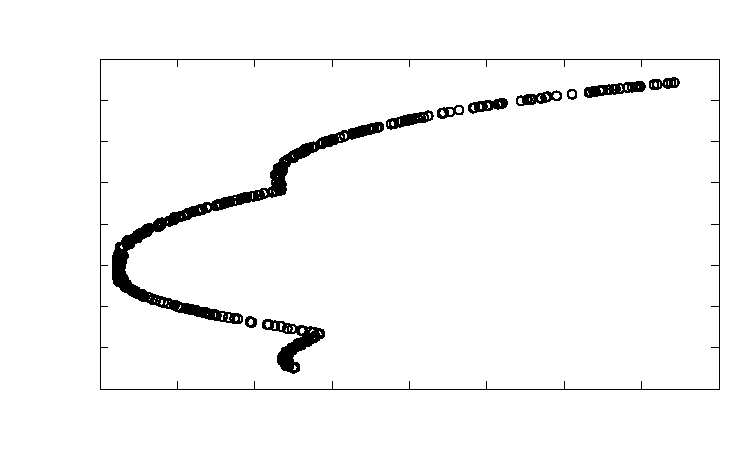
\includegraphics{GRAPH_color_graph2}}%
    \gplfronttext
  \end{picture}%
\endgroup

						}\endgroup
				\caption{B\label{fig:col2}}
			\end{minipage}
			\begin{minipage}[c]{0.5\linewidth}
				\centering
					\begingroup\endlinechar=-1
						\resizebox{\textwidth}{!}{%
							% GNUPLOT: LaTeX picture with Postscript
\begingroup
  \makeatletter
  \providecommand\color[2][]{%
    \GenericError{(gnuplot) \space\space\space\@spaces}{%
      Package color not loaded in conjunction with
      terminal option `colourtext'%
    }{See the gnuplot documentation for explanation.%
    }{Either use 'blacktext' in gnuplot or load the package
      color.sty in LaTeX.}%
    \renewcommand\color[2][]{}%
  }%
  \providecommand\includegraphics[2][]{%
    \GenericError{(gnuplot) \space\space\space\@spaces}{%
      Package graphicx or graphics not loaded%
    }{See the gnuplot documentation for explanation.%
    }{The gnuplot epslatex terminal needs graphicx.sty or graphics.sty.}%
    \renewcommand\includegraphics[2][]{}%
  }%
  \providecommand\rotatebox[2]{#2}%
  \@ifundefined{ifGPcolor}{%
    \newif\ifGPcolor
    \GPcolortrue
  }{}%
  \@ifundefined{ifGPblacktext}{%
    \newif\ifGPblacktext
    \GPblacktexttrue
  }{}%
  % define a \g@addto@macro without @ in the name:
  \let\gplgaddtomacro\g@addto@macro
  % define empty templates for all commands taking text:
  \gdef\gplbacktext{}%
  \gdef\gplfronttext{}%
  \makeatother
  \ifGPblacktext
    % no textcolor at all
    \def\colorrgb#1{}%
    \def\colorgray#1{}%
  \else
    % gray or color?
    \ifGPcolor
      \def\colorrgb#1{\color[rgb]{#1}}%
      \def\colorgray#1{\color[gray]{#1}}%
      \expandafter\def\csname LTw\endcsname{\color{white}}%
      \expandafter\def\csname LTb\endcsname{\color{black}}%
      \expandafter\def\csname LTa\endcsname{\color{black}}%
      \expandafter\def\csname LT0\endcsname{\color[rgb]{1,0,0}}%
      \expandafter\def\csname LT1\endcsname{\color[rgb]{0,1,0}}%
      \expandafter\def\csname LT2\endcsname{\color[rgb]{0,0,1}}%
      \expandafter\def\csname LT3\endcsname{\color[rgb]{1,0,1}}%
      \expandafter\def\csname LT4\endcsname{\color[rgb]{0,1,1}}%
      \expandafter\def\csname LT5\endcsname{\color[rgb]{1,1,0}}%
      \expandafter\def\csname LT6\endcsname{\color[rgb]{0,0,0}}%
      \expandafter\def\csname LT7\endcsname{\color[rgb]{1,0.3,0}}%
      \expandafter\def\csname LT8\endcsname{\color[rgb]{0.5,0.5,0.5}}%
    \else
      % gray
      \def\colorrgb#1{\color{black}}%
      \def\colorgray#1{\color[gray]{#1}}%
      \expandafter\def\csname LTw\endcsname{\color{white}}%
      \expandafter\def\csname LTb\endcsname{\color{black}}%
      \expandafter\def\csname LTa\endcsname{\color{black}}%
      \expandafter\def\csname LT0\endcsname{\color{black}}%
      \expandafter\def\csname LT1\endcsname{\color{black}}%
      \expandafter\def\csname LT2\endcsname{\color{black}}%
      \expandafter\def\csname LT3\endcsname{\color{black}}%
      \expandafter\def\csname LT4\endcsname{\color{black}}%
      \expandafter\def\csname LT5\endcsname{\color{black}}%
      \expandafter\def\csname LT6\endcsname{\color{black}}%
      \expandafter\def\csname LT7\endcsname{\color{black}}%
      \expandafter\def\csname LT8\endcsname{\color{black}}%
    \fi
  \fi
  \setlength{\unitlength}{0.0500bp}%
  \begin{picture}(7200.00,4320.00)%
    \gplgaddtomacro\gplbacktext{%
      \put(849,595){\makebox(0,0)[r]{\strut{} 11}}%
      \put(849,912){\makebox(0,0)[r]{\strut{} 11.5}}%
      \put(849,1228){\makebox(0,0)[r]{\strut{} 12}}%
      \put(849,1545){\makebox(0,0)[r]{\strut{} 12.5}}%
      \put(849,1861){\makebox(0,0)[r]{\strut{} 13}}%
      \put(849,2178){\makebox(0,0)[r]{\strut{} 13.5}}%
      \put(849,2495){\makebox(0,0)[r]{\strut{} 14}}%
      \put(849,2811){\makebox(0,0)[r]{\strut{} 14.5}}%
      \put(849,3128){\makebox(0,0)[r]{\strut{} 15}}%
      \put(849,3444){\makebox(0,0)[r]{\strut{} 15.5}}%
      \put(849,3761){\makebox(0,0)[r]{\strut{} 16}}%
      \put(951,409){\makebox(0,0){\strut{} 1.5}}%
      \put(1694,409){\makebox(0,0){\strut{} 2}}%
      \put(2437,409){\makebox(0,0){\strut{} 2.5}}%
      \put(3179,409){\makebox(0,0){\strut{} 3}}%
      \put(3922,409){\makebox(0,0){\strut{} 3.5}}%
      \put(4665,409){\makebox(0,0){\strut{} 4}}%
      \put(5408,409){\makebox(0,0){\strut{} 4.5}}%
      \put(6150,409){\makebox(0,0){\strut{} 5}}%
      \put(6893,409){\makebox(0,0){\strut{} 5.5}}%
      \csname LTb\endcsname%
      \put(144,2178){\rotatebox{-270}{\makebox(0,0){\strut{}Y-J}}}%
      \csname LTb\endcsname%
      \put(3922,130){\makebox(0,0){\strut{}J-H}}%
      \put(3922,4040){\makebox(0,0){\strut{}Redshift 8.5--10.1}}%
    }%
    \gplgaddtomacro\gplfronttext{%
    }%
    \gplbacktext
    \put(0,0){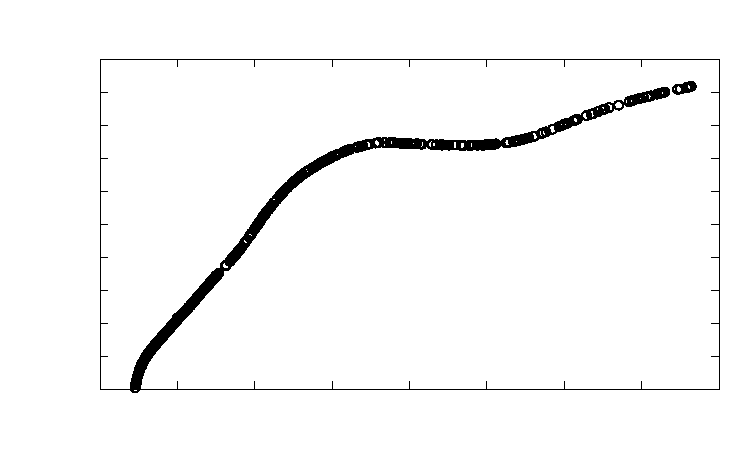
\includegraphics{GRAPH_color_graph3}}%
    \gplfronttext
  \end{picture}%
\endgroup

						}\endgroup
				\caption{C\label{fig:col3}}
			\end{minipage}
			\begin{minipage}[c]{0.5\linewidth}
				\centering
					\begingroup\endlinechar=-1
						\resizebox{\textwidth}{!}{%
							% GNUPLOT: LaTeX picture with Postscript
\begingroup
  \makeatletter
  \providecommand\color[2][]{%
    \GenericError{(gnuplot) \space\space\space\@spaces}{%
      Package color not loaded in conjunction with
      terminal option `colourtext'%
    }{See the gnuplot documentation for explanation.%
    }{Either use 'blacktext' in gnuplot or load the package
      color.sty in LaTeX.}%
    \renewcommand\color[2][]{}%
  }%
  \providecommand\includegraphics[2][]{%
    \GenericError{(gnuplot) \space\space\space\@spaces}{%
      Package graphicx or graphics not loaded%
    }{See the gnuplot documentation for explanation.%
    }{The gnuplot epslatex terminal needs graphicx.sty or graphics.sty.}%
    \renewcommand\includegraphics[2][]{}%
  }%
  \providecommand\rotatebox[2]{#2}%
  \@ifundefined{ifGPcolor}{%
    \newif\ifGPcolor
    \GPcolortrue
  }{}%
  \@ifundefined{ifGPblacktext}{%
    \newif\ifGPblacktext
    \GPblacktexttrue
  }{}%
  % define a \g@addto@macro without @ in the name:
  \let\gplgaddtomacro\g@addto@macro
  % define empty templates for all commands taking text:
  \gdef\gplbacktext{}%
  \gdef\gplfronttext{}%
  \makeatother
  \ifGPblacktext
    % no textcolor at all
    \def\colorrgb#1{}%
    \def\colorgray#1{}%
  \else
    % gray or color?
    \ifGPcolor
      \def\colorrgb#1{\color[rgb]{#1}}%
      \def\colorgray#1{\color[gray]{#1}}%
      \expandafter\def\csname LTw\endcsname{\color{white}}%
      \expandafter\def\csname LTb\endcsname{\color{black}}%
      \expandafter\def\csname LTa\endcsname{\color{black}}%
      \expandafter\def\csname LT0\endcsname{\color[rgb]{1,0,0}}%
      \expandafter\def\csname LT1\endcsname{\color[rgb]{0,1,0}}%
      \expandafter\def\csname LT2\endcsname{\color[rgb]{0,0,1}}%
      \expandafter\def\csname LT3\endcsname{\color[rgb]{1,0,1}}%
      \expandafter\def\csname LT4\endcsname{\color[rgb]{0,1,1}}%
      \expandafter\def\csname LT5\endcsname{\color[rgb]{1,1,0}}%
      \expandafter\def\csname LT6\endcsname{\color[rgb]{0,0,0}}%
      \expandafter\def\csname LT7\endcsname{\color[rgb]{1,0.3,0}}%
      \expandafter\def\csname LT8\endcsname{\color[rgb]{0.5,0.5,0.5}}%
    \else
      % gray
      \def\colorrgb#1{\color{black}}%
      \def\colorgray#1{\color[gray]{#1}}%
      \expandafter\def\csname LTw\endcsname{\color{white}}%
      \expandafter\def\csname LTb\endcsname{\color{black}}%
      \expandafter\def\csname LTa\endcsname{\color{black}}%
      \expandafter\def\csname LT0\endcsname{\color{black}}%
      \expandafter\def\csname LT1\endcsname{\color{black}}%
      \expandafter\def\csname LT2\endcsname{\color{black}}%
      \expandafter\def\csname LT3\endcsname{\color{black}}%
      \expandafter\def\csname LT4\endcsname{\color{black}}%
      \expandafter\def\csname LT5\endcsname{\color{black}}%
      \expandafter\def\csname LT6\endcsname{\color{black}}%
      \expandafter\def\csname LT7\endcsname{\color{black}}%
      \expandafter\def\csname LT8\endcsname{\color{black}}%
    \fi
  \fi
  \setlength{\unitlength}{0.0500bp}%
  \begin{picture}(7200.00,4320.00)%
    \gplgaddtomacro\gplbacktext{%
      \put(645,595){\makebox(0,0)[r]{\strut{} 10}}%
      \put(645,947){\makebox(0,0)[r]{\strut{} 15}}%
      \put(645,1299){\makebox(0,0)[r]{\strut{} 20}}%
      \put(645,1650){\makebox(0,0)[r]{\strut{} 25}}%
      \put(645,2002){\makebox(0,0)[r]{\strut{} 30}}%
      \put(645,2354){\makebox(0,0)[r]{\strut{} 35}}%
      \put(645,2706){\makebox(0,0)[r]{\strut{} 40}}%
      \put(645,3057){\makebox(0,0)[r]{\strut{} 45}}%
      \put(645,3409){\makebox(0,0)[r]{\strut{} 50}}%
      \put(645,3761){\makebox(0,0)[r]{\strut{} 55}}%
      \put(747,409){\makebox(0,0){\strut{} 0}}%
      \put(1515,409){\makebox(0,0){\strut{} 2}}%
      \put(2284,409){\makebox(0,0){\strut{} 4}}%
      \put(3052,409){\makebox(0,0){\strut{} 6}}%
      \put(3820,409){\makebox(0,0){\strut{} 8}}%
      \put(4588,409){\makebox(0,0){\strut{} 10}}%
      \put(5357,409){\makebox(0,0){\strut{} 12}}%
      \put(6125,409){\makebox(0,0){\strut{} 14}}%
      \put(6893,409){\makebox(0,0){\strut{} 16}}%
      \csname LTb\endcsname%
      \put(144,2178){\rotatebox{-270}{\makebox(0,0){\strut{}f150w-f200w}}}%
      \csname LTb\endcsname%
      \put(3820,130){\makebox(0,0){\strut{}f115w-f150w}}%
      \put(3820,4040){\makebox(0,0){\strut{}Redshift 10--14}}%
    }%
    \gplgaddtomacro\gplfronttext{%
    }%
    \gplbacktext
    \put(0,0){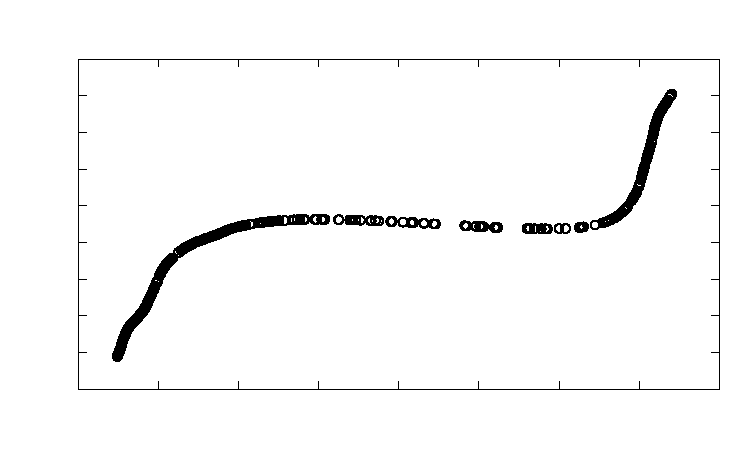
\includegraphics{GRAPH_color_graph4}}%
    \gplfronttext
  \end{picture}%
\endgroup

						}\endgroup
				\caption{D\label{fig:col4}}
			\end{minipage}
			\caption{Graphs showing the colour-colour regions for \\
			(A) z=6-7.5. The colour window was defined as $f070w-f090w{\ge}3.257$ and $f090w-f115w{\le}8.242$,\\
			(B) z=7.5-8.5. The colour window was defined as $f090w-f115w{\ge}8.251$ and $f115w-f150w{\le}2.869$, \\
			(C) z=8.54-10.1. The colour window was defined as $Y-J{\ge}11.019$ and $J-H{\le}5.298$, \\
			(D) z=10-14. The colour window was defined as $f115w-f150w{\ge}14.439$ and $f150w-f200w{\le}14.815$}
		\end{figure}
	%subsection Results_for_Colour (end)

	\subsection{Interpretation of Colour Results}
	\label{sub:Interp_Colour}
		Constraining a colour window for observations turned out to be a challenging task. The filter 275w on James Webb didn't work properly in Hyperz; some magnitudes came out as 99.0 which is the default answer if there was an error; other magnitudes were above 100. As the source of this error could not be found, the range of redshift 14 to 15 was taken from the colour window results. The colour window results  shown in Figures~\ref{fig:col1},~\ref{fig:col2},~\ref{fig:col3} and~\ref{fig:col4} are much higher than expected results such as the colour windows in \cite{lorenzoni2013constraining}. Something must be wrong with the technique that was used to find the colours, however in defense of the results, the assumptions made as described in the sections above were reasonably fair for the timescale of the project. It's hard to say if there is one set of inputs or parameters that were the main source of error.  The shape of the distribtution of the galaxies is odd but seems to follow a pattern for each redshift range, which remains unexplained. The other peculiar characteristic of the diagrams is that all the galaxies appear on a mainly continous line, as opposed to being distributed in a certain area. Having done some basic tests, the cause of this appears to be due to setting the age of the galaxies at the same redshift to be the same; as soon as the age was randomised to some time between the formation redshift and the observed redshift, the galaxies were more spread out. However these galaxies appeared `inside' the colour window, so this doesn't appear to have affected the determination of the colour windows.
	%section Interpetation_of_colour_results (end)
%section Photometry_and_colour (end)

    %!TEX root = mainfile.tex

\section{Contaminants} % (fold)
\label{sec:contaminants}
    \subsection{Low Mass Stars} % (fold)
    \label{sub:low_mass_stars}
        These can easily be identified due to the high resolution imaging provided by \ldots. The Point-spread function (PSF) obtained will allow us to determine which sources are point-like and which are extended. We should be able to avoid significant contamination by removing any point-like sources from the results as all galaxies should have a great enough diameter.
    % subsection low_mass_stars (end)

    \subsection{Spurious Sources} % (fold)
    \label{sub:spurious_sources}
        By stipulating that we will be requiring detections in two bands the influence of spurious sources will be negligible. Finding detections in 2 bands at reasonable confidence interval (?3sig?) is very improbable. By inspecting the negative with the same requirements for detection we are able to identify any such sources easily\cite{Bouwens2011}.
    % subsection spurious_sources (end)

    \subsection{Supernovae and other transient sources} % (fold)
    \label{sub:supernovae_and_other_transient_sources}
        Events such as Supernovae happen incredibly quickly releasing a vast amount of energy, as seen in figure~\ref{fig:SNe_1987a}. These events can spoil images due to their short duration by introducing new data in only a portion of the sample. These effects are usually only considered when taking exposures years apart or when combining multiple sources over a long time scale. Such events are very unlikely to contaminate our results as we propose to take our images close in time.
        \begin{figure}[!htb]
            \centering
            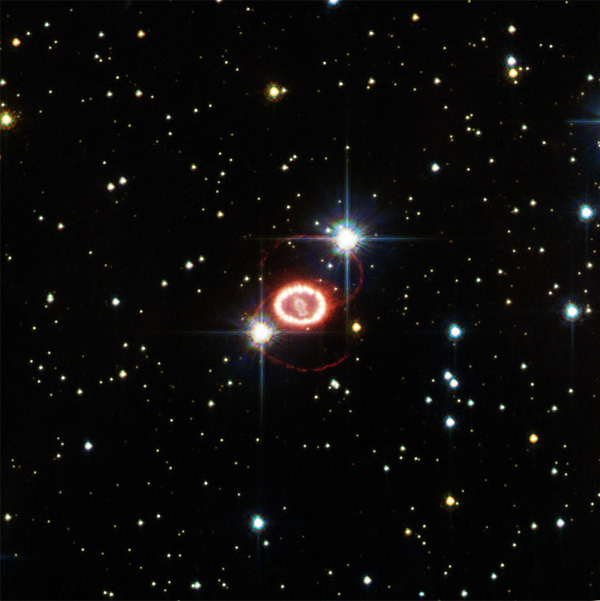
\includegraphics[width=0.6\textwidth]{../Images/SNe_1987a.jpg}
            \caption{The shock wave from Supernova 1987a imaged by HST in 2006.\label{fig:SNe_1987a}}
        \end{figure}
    % subsection supernovae_and_other_transient_sources (end)

    \subsection{Lower Redshift Sources and photometric scattering} % (fold)
    \label{sub:lower_redshift_sources_and_photometric_scattering}
        This category is likely to provide the greatest source of contamination for the surveyed area. It will do so increasingly at high redshifts where its affect on the faintest magnitudes is most greatly felt. Its affect is most influential with a small S/N ratio for the observations, by fixing this at a level of S/N = \ldots we can be confident that the contamination will be low. Detecting a source in another band such as b435, v606, i775 for YJH photometry would class it as a contaminant and then should be removed from sample.
    % subsection lower_redshift_sources_and_photometric_scattering (end)

% section contaminants (end)

    %!TEX root = mainfile.tex

\subsection{CMB Secondary Anisotropies} % (fold)
\label{sub:cmb_secondary_anisotropies}
	Over large angular scales, the CMB polarization contains key information concerning the evolution of ionization during the EoR. The CMB photons released during recombination experienced considerable Thomson scattering off of free electrons. This scattering is imprinted onto the CMB anisotropy map introducing secondary anisotropies. This has the effect of removing anisotropies on smaller scales and introducing polarization anisotropies. By comparing the anisotropies observed with models of the CMB without reionization it is possible to determine the electron column density during the EoR. Using this method it is possible to calculate the period over which reionization took place. It is also possible to make measurements of the metal enrichment history of the IGM at the EoR. On-resonance scattering off metals and the influence of inverse Compton scattering (the Sunyaev-Zel'dovich effect) introduced additional signals into the CMB\cite{Monteagudo2006}. Studies in this field are expected to get a new impetus in the coming years with the results from the Planck telescope giving greater insight into the CMB map.
% subsection cmb_secondary_anisotropies (end)

    %!TEX root = mainfile.tex

\section{Other methods for detecting Re-ionization (21cm)} % (fold)
\label{sec:other_methods_for_detecting_re-ionization}

    \subsection{Hydrogen 21cm line} %fold
    \label{sub:Hydrogen_21cm}
        The method of using the hyperfine transition of neutral Hydrogen from the ground state to study re-ionization could provide much more detail about the process of re-ionization than the Lyman break dropout method.

         \subsubsection{Hyperfine transition of Hydrogen} %fold
         \label{subsub:Hyperfine_Hydrogen}
            The Hyperfine transition corresponds to the change in the two hyperfine levels of the hydrogen 1s ground state with an energy difference of \SI{5.87433}{\micro\electronvolt}.

            FURTHER RESEARCH FROM BOOK AND DIAGRAM
        %subsubsection Hyperfine_transition_of_Hydrogen (end)

        \subsubsection{Method of Measuring \SI{21}{\centi\metre}} %fold
    	\label{subsub:Measuring_21cm}
            To observe the hydrogen \SI{21}{\centi\metre} absorption spectrum, radio sources are needed. If the radio source is located before or during the epoch of re-ionization, it's possible to see the structure of neutral hydrogen gas along the line of sight using the absorption of the \SI{21}{\centi\metre} line in the radio spectrum. Several features should be apparent blueward of the redshifted \SI{21}{\centi\metre} line: a decrement of flux due to the optical depth of the IGM along the line of sight at a particular redshift, which will vary along the line of sight due to changes in density and the ionization of the IGM and there will be areas of transmission and absorption due to `bubbles' of photoionized hydrogen and dense areas or clouds of hydrogen. Currently there are several arrays of radio telescopes planned for observing the 21cm. LOFAR, GMRT, EDGES, PAPER, MWA, SKA.
        %subsubsection Measuring_21cm (end)

        \subsubsection{Advantages/disadvantages} %fold
    	\label{subsub:Advantages_disadvantages_21cm}
            The major advantage of observing the \SI{21}{\centi\metre} forest over the Lyman break technique is that it is possible to study the history of the re-ionization far more accurately, this is because the Gunn Peterson trough reaches zero flux for the lyman break technique with only a small fraction of hydrogen in the line of sight needed.

            The main reason this study did not use the \SI{21}{\centi\metre} absorption spectrum is that it requires far more careful consideration of the IGM. This is quite a different setup from the broad assumptions that can be made for the lyman break technique, and therefore it was thought that with the time constraint of the project. MORE NEEDED HERE
        %subsubsection Advantages_disadvantages_21cm(end)

    %subsection Hydrogen_21cm (end)

    \subsection{Other methods (tbc)} %fold
    \label{sub:Other_Methods_Re-ionization}

    %subsection Other_Methods_Re-ionization (end)

%section other_methods_for_detecting_re-ionization (end)

    %!TEX root = mainfile.tex

\subsection{Observational Gravitational Lensing} % (fold)
\label{sec:observational_gravitational_lensing}
	Gravitational lensing will enhance the observing capabilities of any telescope used allowing some of the most distant objects in the universe to be seen. Since one of the aims of this project is to push current boundaries and observe objects at as yet unexplored redshifts, lensing will prove to be a very useful tool. Lensed sources at redshifts above 7 tend to be magnified by a factor of 5 to 10 over an area of 1 square arcminute, however this magnification can be as much as 30 times for certain source locations\cite{magnification}. Two routes were considered to include gravitational lensing in the observing strategy: either new lenses could be located or lenses found by other surveys could be selected. This section lays out the properties desired for the lenses chosen and the arguments for each of these options.

	\subsubsection{Constraints on the Lenses} % (fold)
	\label{sub:constraints_on_the_lenses}
		The lenses used will be chosen depending on the suitability of their properties for the observing strategy. Firstly, the area of the sky in which the lenses lie must be chosen carefully, particularly if a ground based telescope is used. The region of sky must be chosen to be compatible with the direction in which the telescope(s) used for the deep survey are able to point. For a space based telescope, this is not a major issue since they are not confined by the Earth’s motion. Any regions with bright foreground contaminants would be ruled out and the lenses would be chosen such that they are distributed across the sky in order to reduce the effect of cosmic variance. Another factor that must be accounted for is that the lensing cross section of an object is directly dependent on its mass, as shown in Figure~\ref{fig:Lensing_cross_section_as_a_function_of_mass}\cite{Optimal_mass_configurations}. This would suggest that the lenses chosen should be very massive and are therefore likely to be galaxy clusters.
		\begin{figure}[!htbp]
			\centering
				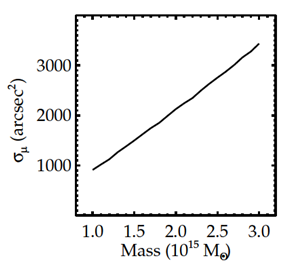
\includegraphics[width=0.4\textwidth]{../Images/Lensing_cross_section_as_a_function_of_mass.png}
			\caption[Lensing cross section as a function of mass]{\cite{Optimal_mass_configurations}Plot of the lensing cross section as a function of mass for a spherical halo at $z=0.5$. The dependence of cross section on mass can be clearly seen, indicating that the more massive a cluster, the better a lens it will be.\label{fig:Lensing_cross_section_as_a_function_of_mass}}
		\end{figure}

		The source magnification is also sensitively dependent on the lens redshift, though constraining this is less straightforward as there is a trade-off between Einstein angle and shear. On the one hand, the Einstein angle, an indicator of the strength of a lens, increases as the lens redshift decreases. Figure~\ref{fig:Einstein_angle_as_a_function_of_source_redshift} shows how lens redshift varies with Einstein angle. The point at which each curve crosses the x-axis is the lens redshift, since no lensing occurs when the source and lens redshifts are equal. For each value of lens redshift, the Einstein angle increases rapidly at source redshifts slightly greater than that of the lens, and then quickly saturates\cite{Constraining_source_redshift_distributions}. The lower the redshift of the lens, the higher the saturation value, suggesting lower lens redshifts are the best.
		\begin{figure}[!htbp]
			\centering
				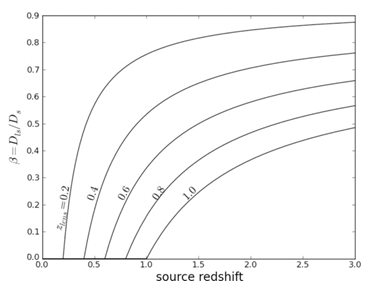
\includegraphics[width=0.5\textwidth]{../Images/Einstein_angle_as_a_function_of_source_redshift.png}
			\caption[Einstein angle as a function of source redshift]{\cite{Constraining_source_redshift_distributions} Plot of Einstein angle against source redshift. Again, each line corresponds to a different lens redshift. The point at which each line crosses the x-axis is the lens redshift, since at the lens, the magnification of the source is equal to 0.\label{fig:Einstein_angle_as_a_function_of_source_redshift}}
		\end{figure}

		However, the extent to which the images are distorted is not taken into account. The shear caused by a lens at a particular redshift is given by
		\begin{align}
			\gamma(r) &= \frac{4\pi G}{c^2}\frac{D_{LS}D_L}{D_S}\left( \overline{\Sigma}(<r)-\Sigma(r) \right)
		\end{align}
		where $\overline{\Sigma}(<r)$ is the mean projected surface mass density within r and $\Sigma(r)$ the projected surface mass density at $r$. Keeping the radius (and therefore surface mass density) constant, Figure~\ref{fig:shear_as_a_function_of_source_redshift} shows the dependence of shear on source redshift at the same fixed lens redshifts as the plot above. lens redshifts as the plot above. It can be seen from this plot, that at low source redshifts, the shear distortion is immeasurably small. As the redshift increases to around 0.5, the clusters at the lowest redshifts cause some significant distortion. Once the source redshift is greater than 1, shear distortion is seen around clusters at all the lens redshifts plotted\cite{Constraining_source_redshift_distributions}.
		\begin{figure}[!htbp]
			\centering
				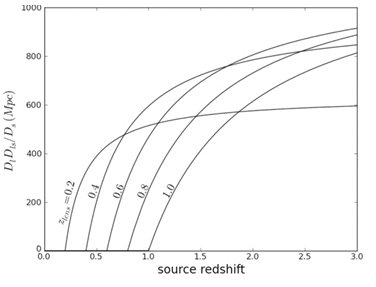
\includegraphics[width=0.5\textwidth]{../Images/Shear_as_a_function_of_source_redshift.png}
			\caption[Shear as a function of source redshift]{\cite{Constraining_source_redshift_distributions}A plot of shear against source redshift, with each line representing a different lens redshift. The point at which the lines cross the x-axis is the lens redshift, since at the lens, the magnification of the source is equal to 0.\label{fig:shear_as_a_function_of_source_redshift}}
		\end{figure}

		It has also been found that giant arcs are most likely to form behind higher redshift lenses, as shown in Figure~\ref{fig:Arc_probability}. Giant arcs are observed in systems where the shear is large. Lensing clusters at a redshift above 0.5 have been found to have an arc formation probability up to 3 times that of lower redshift lenses. Clusters observed at $z>0.5$ have also been found as a general rule to be less massive than closer clusters, indicating that clusters at this redshift are more efficient lenses. As a result, a judicious choice of lens redshift must be made to optimise both lensing strength and distortion for the best chance of observing high redshift galaxies\cite{wu_and_chiueh}.
		\begin{figure}[!htbp]
			\centering
				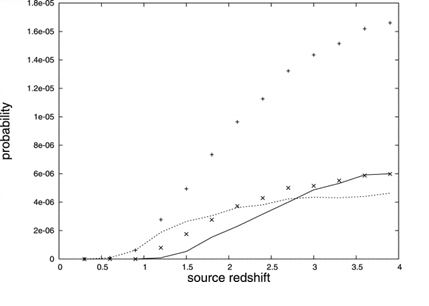
\includegraphics[width=0.5\textwidth]{../Images/Arc_probability.png}
			\caption[Arc probability]{\cite{wu_and_chiueh}Plot of the arc probability against source redshifts in four different lens intervals, $0.14\le z_L\le 0.45$ (dotted line), $0.49\le z_L\le 0.68$ (crosses), $0.73\le z_L\le 0.94$ (solid line), and $0.14\le z_L\le 0.94$ (plus signs).\label{fig:Arc_probability}}
		\end{figure}
	% subsection constraints_on_the_lenses (end)

	\subsubsection{Locating New Lenses} % (fold)
	\label{sub:locating_new_lenses}
		Locating new lenses would be advantageous in that the lenses could be chosen with the tight constraints specified above such that their properties are tailored to suit the needs of our strategy. The lenses would be selected using some form of wide survey by means of their strong lensing properties since objects that lense strongly are likely to be better for observing very faint sources. The parameters describing the lenses located would not be known so calculations to find these must be carried out. Taking the Einstein radius to be the average distance of the arcs from the centre of the lens, and assuming that most of the mass of the cluster is enclosed within this radius, an estimate of the mass can be found from
		\begin{align}
			M &= \Sigma_c\pi \theta_E^2 \label{eq:new_lens_mass_estimate}
		\end{align}
		The critical surface density, as defined in equation~(\ref{eq:new_lens_mass_estimate}) can be found when the source redshift is known and the magnification of the source can then be calculated as detailed in Section~\ref{sec:gravitational_lensing}.
	% subsection locating_new_lenses (end)

	\subsubsection{Using Known Lenses} % (fold)
	\label{sub:using_known_lenses}
		The second option, selecting known lenses has the advantage that the masses and velocity dispersions would already be well determined, allowing an accurate calculation of the magnification to be made. Examples of surveys that have been carried out previously include the Cluster Lens And Supernova survey with Hubble (CLASH)\cite{CLASH} and the MAssive Cluster Survey (MACS)\cite{MACS}. There are only a limited number of massive clusters known, however even with the small sample available, many interesting sources have already been observed for example a candidate $z\approx11$ galaxy behind cluster MACSJ0647.7+7015\cite{CLASH_z11_candidate}. Unless a wide survey is carried out as part of the observing strategy, using known lenses would significantly reduce the observing time required for the strategy compared to requiring an additional survey to locate new lenses. Both MACS and CLASH select their source using x-rays in order to obtain an unbiased distribution of masses, however, for this strategy the lenses would be chosen from these catalogues based on their masses and lensing properties.

	% subsection using_known_lenses (end)
% section observational_gravitational_lensing (end)

    %!TEX root = mainfile.tex
\subsection{Spectroscopy} % (fold)
\label{sec:spectroscopy}
	The spectrum of typical high redshift galaxy can be seen in Figure~\ref{fig:high_redshift_galaxy_spectrum}.
	\begin{figure}[!htbp]
		\centering
			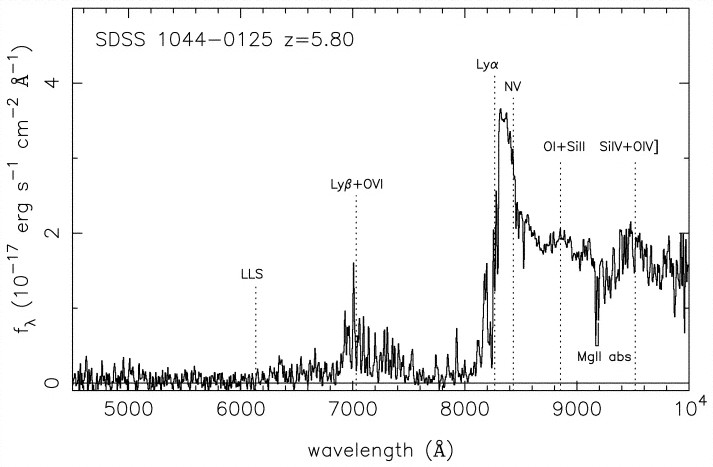
\includegraphics[width=0.7\textwidth]{../Images/high_redshift_galaxy_spec.jpg}
		\caption{\label{fig:high_redshift_galaxy_spectrum}}
	\end{figure}

	The distinct drop in emission is due to the presence of neutral hydrogen around the galaxies, known as the Gunn Peterson trough. Therefore the galaxies where formed before the start of re-ionisation. This is discussed in detail in Section~\ref{sec:the_gunn_peterson_effect}. However this particular feature in the spectra is of great importance here. The wavelength at which this drop occurs corresponds to the amount of energy required for an electron to transition between the first two energy levels in neutral hydrogen. This is known as the Lyman-$\alpha$ transition line and has a rest frame wavelength here on earth of \SI{1216}{\angstrom}\cite{rauch2001lyman}. However, the actual wavelength that this drop occurs in the spectrum of the galaxy being studied will be much longer. In Figure~\ref{fig:high_redshift_galaxy_spectrum}, it is closer to \SI{8000}{\angstrom}.This is due to the fact that the light is red shifted effectively stretching the wavelength. Indeed, the observed wavelength of the Lyman-$\alpha$ transition line will be in the infrared range. If this wavelength can be measured precisely then the redshift of the galaxy can be calculated\cite{rauch2001lyman}. This is done using the relation,
	\begin{align}
		1+z &= \frac{\lambda_{\text{observed}}}{\lambda_{\text{emitted}}} \label{eq:spectroscopy}
	\end{align}
	Hence, spectroscopy can be used to confirm the high-red shift galaxy candidates that are identified via photometry. In essence it is high resolution photometry.

	An astronomical spectrograph splits or disperses light from a source into its constituent wavelengths. Therefore it has to have some means of dispersing the light. The simplest way this can be achieved is via a prism. This exploits the fact that different wavelengths are diffracted via different amounts. However, they are rarely used by themselves in astronomical spectroscopy due to their inefficiency. Only about 10\% of the light incident upon them actually gets dispersed. Moreover, the dispersion is nonlinear causing some light to be dispersed more than others. Therefore, the universal dispersing medium used in astronomical spectroscopy is the diffraction grating. A diffraction grating consists of a large number of equidistant parallel lines ruled onto a transparent glass plate. The incident light cannot travel through the grating, but is instead channelled along the parallel lines. As the light reaches the end of the lines it is diffracted producing a series of wavelets in accordance with Huygens’s Principle. These either constructively or destructively interfere producing a series of maxima or minima. Again, different wavelengths of light will be diffracted through different angles. Therefore each maximum (order) can be thought of as the image of the galaxy split into its constituent wavelengths. As a general rule, the first maximum is projected onto the CCD equipment of the telescope and used to calculate the redshift. This is due to the fact it has the highest intensity. Figures~\ref{fig:grating_to_split_light} and~\ref{fig:grating_close_up} below show a schematic of a grating being used to split light
	\begin{figure}[!htbp]
		\begin{minipage}[c]{0.5\linewidth}
			\centering
			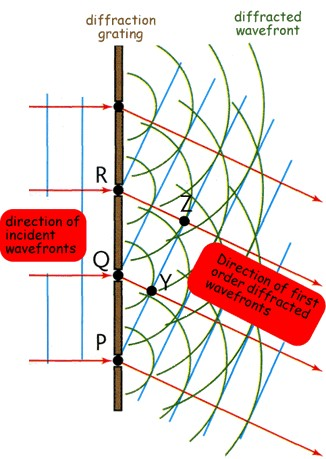
\includegraphics[width=0.7\textwidth]{../Images/grating_to_split_light.jpg}
			\caption{\label{fig:grating_to_split_light}}
		\end{minipage}
		\begin{minipage}[c]{0.5\linewidth}
			\centering
			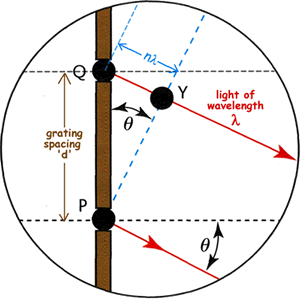
\includegraphics[width=0.7\textwidth]{../Images/grating_close_up.png}
			\caption{\label{fig:grating_close_up}}
		\end{minipage}
	\end{figure}

	Angles at which the orders occur can be found using the grating equation,
	\begin{align}
		n\lambda &= d(\sin\theta + \sin\phi)
	\end{align}
	Where $\phi$ is the angle of incidence between the light and the grating, $\theta$ is the angle of dispersion and $d$ is the grating spacing. The value of $n\lambda$ is an integer number of wavelengths of the incident light.

	Before light reaches either a prism or diffraction grating it is often sent through a fixed slit. This is a mask with a narrow rectangular aperture that is placed in the focal plane of the telescope. The slit has two main functions. First and foremost it isolates a portion of the sky of interest so that only light that falls on the slit may enter the spectrograph. This is important as it means the spectra from different parts of a galaxy cannot enter the spectrograph, overlap and thus contaminate each other. Second, the slit provides a stable spectral resolution. Without the slit the spectral resolution would be defined by the width of the galaxy or star. However, this varies with time so the spectral line width would vary with time. This would make detailed analysis of the spectrum almost impossible. If on the other hand a slit is used, the spectrum becomes an infinite number of images of the slit, and not the galaxy or star etc. As the slit width is constant, the spectral resolution remains stable.

	In between the slit and dispersion medium usually sits a collimator. The light from the slit diverges and if left would hit the grating or prism at differing angles of incidence making the resulting spectrum useless. Therefore a collimator is used to turn the diverging light back to parallel. Figure~\ref{fig:nirspec_jwst} below shows the set-up for NIRspec on the JWST.
	\begin{figure}[!htbp]
		\centering
			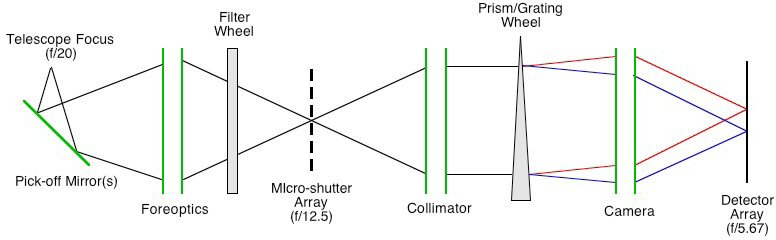
\includegraphics[width=0.8\textwidth]{../Images/nirspec_jwst.jpeg}
		\caption{\label{fig:nirspec_jwst}}
	\end{figure}

	Grisms are a combination of both diffraction gratings and prisms. In some cases they enable spectroscopy and photometry to be undertaken simultaneously. This is achieved by using the dispersed and undispersed light that they produce. This means that exposure times can be shortened when viewing and confirming high red shift galaxy candidates.
% section spectroscopy (end)



    \section{Ground Based versus Space Based Telescopes} % (fold)
\label{sec:ground_based_versus_space_based_telescopes}
	Ground based telescopes are seeing limited which is a resolving limitation due to distortion caused by the atmosphere. Light is scattered by the atmosphere and so detecting a source by these telescopes can be difficult. There is also the limitation of considerably more background light, compared to what is measured by space telescopes. To minimise these limitations, ground based telescopes are usually located at high altitude at locations such as Mauna Kea, Hawaii. The main advantage of ground based telescopes is that they can be built to very large sizes with telescopes with a primary diameter of around 30\,metres on the periphery. This cannot be achieved by space telescopes as the cost of transport to space would be very large and the telescope may well be damaged during this transportation.

	Space based telescopes are diffraction limited, i.e.\ the only limitation is whether they can resolve the object being observed. Taking the source as a point spread function, the light from the source will spread out and so the telescope must determine the source. This is important as light from other sources in the sky may almost overlap and so the diffraction gives the angle in the sky which can be resolved. Thus if the diffraction angle, the smallest angle between two objects can be resolved, is small, the better the telescope. Should two sources fall within this diffraction angle when looking into the sky, the telescope will not be able to resolve the two objects and so one cannot be distinguished from another. The diffraction angle can be calculated using the formula below:
	\begin{align}
		\Delta\theta= \frac{(1.22 \lambda)}D
	\end{align}

	This also shows that the larger the diameter, the smaller the diffraction angle will be and so the better the telescope will be at resolving sources.

	The main disadvantage of space based telescope is that they must be transported into space. This is usually done with the aid of a rocket and so the cost of achieving this can be considerable. The telescope may also be damaged during this transportation and so this limits the size of the telescope as a smaller size will mean a smaller chance of being damaged. The James Webb Space Telescope scheduled for launch in 2018 consists of a 6.5 metre primary mirror made up of multiple mirrors that will unfold once it is in space. Despite this folding up of the telescope, the primary mirror size is still small relative to some ground based ones currently in use such as the VLT (primary mirror of 8.2\,metres) and is considerably smaller than some proposed for the future such as the EELT (primary mirror 39.3\,metres).


	\subsection{Astronomical Seeing} % (fold)
	\label{sub:astronomical_seeing}
		Plane waves from a source being observed are distorted by the Earth’s atmosphere and so upon reaching a telescope within the atmosphere are slightly perturbed and so the image formed is blurred. This effect is contributed to by numerous layers where different temperatures or the interaction of different wind speed causes this effect with ‘Seeing’ the term used to describe the total distortion of the wavefront\cite[page~188]{Diffraction_Limited_Imaging_Saha}. This effect is shown below in figure~\ref{fig:Seeing} where a turbulent layer of the atmosphere causes a change in the shape of the wavefront.
		\begin{figure}[ht]
			\centering
			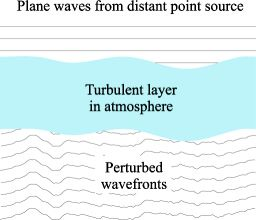
\includegraphics[width=0.4\textwidth]{../Images/Seeing.png}
			\caption{Figure 1}\label{fig:Seeing}
		\end{figure}

		Whilst the resolving power of a telescope is generally largely dependent on its diameter, this seeing limitation becomes the major source of error when resolving a point source from within the Earth’s atmosphere. This is consequently the main limitation for ground based telescopes which are therefore known as being seeing limited. A point spread function (PSF) imaged in these circumstances produces what is known as a seeing disc due to the atmospheric turbulence and the most common measurement used to describe this effect is the full width at half maximum, hereafter the FWHM, shown below in figure~\ref{fig:FWHM} where a peak shape is produced by this overall blurring of the source. When measuring the flux arriving at the CCD from a particular source, an area of radius four times the FWHM is recorded over and so a larger value of FWHM also increases the integration time required to observe the source.
		\begin{figure}[ht]
			\centering
			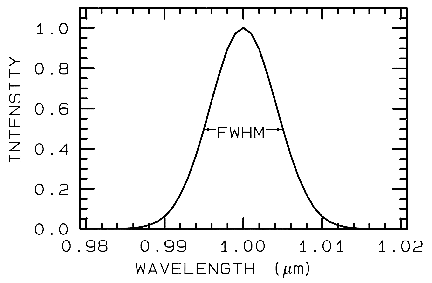
\includegraphics[width=0.5\textwidth]{../Images/FWHM.png}
			\caption{Figure 1}\label{fig:FWHM}
		\end{figure}
	% subsection astronomical_seeing (end)

	\subsection{The Future of Ground Based Telescopes} % (fold)
	\label{sub:the_future_of_ground_based_telescopes}
		The main disadvantage of ground based telescopes compared to space based telescopes is the poorer resolution due to the distortion caused by the atmosphere or astronomical seeing. The introduction of adaptive optics however, should help resolve this issue and allow ground based telescopes to be only diffraction limited similar to space based ones. This, combined with the large diameter mirrors currently in the pipeline such as for the European Extremely Large Telescope (E-ELT), a primary mirror of 39.3 metres, and the Giant Magellan Telescope (GMT), a primary mirror of 25\,metres, ensure ground based telescopes hold a place in the future of space observation, even if just to compliment space based ones. The larger mirrors ensure a greater light collecting power, receiving more photons for the source being observed and so significantly reducing the observing time required. These large diameter mirrors are currently only possible for ground based telescopes and so provide them with a distinct advantage over space based ones.

		\subsubsection{Adaptive Optics} % (fold)
		\label{ssub:adaptive_optics}
			As described earlier in astronomical seeing, light passing through the atmosphere from a source, such as a distant galaxy, is perturbed due to atmospheric turbulence and so the images produced by ground based telescopes are blurred. Adaptive optics works by first sensing the wavefront perturbations and then counteracting this blurring in real time thus enabling the telescopes to hold a much larger resolving power. This system will be used on future ground based telescopes ensuring they are no longer limited by the ability to resolve a source. An example of how this is set up, as on the Subaru Telescope, is shown below in figure~\ref{fig:AdaptiveOptics}.
			\begin{figure}[ht]
				\centering
				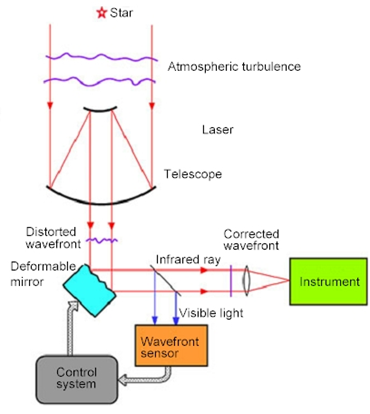
\includegraphics[width=0.6\textwidth]{../Images/AdaptiveOptics.png}
				\caption{Figure 1}\label{fig:AdaptiveOptics}
			\end{figure}

			The wavefront sensor (WFS) measures the distortions in the incoming wavefront of light. This then provides the measured information to an actuator control computer identified in figure~\ref{fig:AdaptiveOptics} as the control system. This then adjusts the shape of the adjustable mirror to effectively correct the wavefront reaching the telescope\cite{Diffraction_Limited_Imaging_Saha}.  The wavefront sensor can measure the distortions introduced into the wavefront on the timescale of a few milliseconds with the information then computed and the shape of the mirror adjusted accordingly. The correction process should therefore be completed in a time similar to the time between the changes of the wavefront thus ensuring the distortion is compensated for.
		% subsubsection adaptive_optics (end)
	% subsection the_future_of_ground_based_telescopes (end)
% section ground_based_versus_space_based_telescopes (end)


\section{Observation Times} % (fold)
\label{sec:observation_times}
	The main aim of this project is to produce an observing strategy to view some of the earliest galaxies in the universe. An important aspect of this is therefore the viewing of the galaxies themselves and the time it will take to do so. The time required to view these galaxies depends not only on the telescope being used, but also the devices used. A charged coupled device (CCD) will be used to measure the light from these sources and so to calculate the times required to view these galaxies, these must be understood in more detail. The telescope or telescopes used during the observation of these galaxies will have different properties which will affect the time required to view the source. Some of these are mentioned below.

	\subsection{Telescope Properties} % (fold)
	\label{sub:telescope_properties}

		\subsubsection{Mirror Reflectivity} % (fold)
		\label{ssub:mirror_reflectivity}
			One such factor that will increase the time required to view a source is the reflectivity of the mirrors used on the telescope. The mirror reflectivity, given as a percentage, is the amount of light reflected by the mirror. Some of the light is absorbed as the mirror is not one hundred per cent efficient meaning not all photons striking the mirror reach the CCD. The reflectivity differs depending on the material used on the surface of the mirrors. Various optical coatings are produced and used depending on the wavelengths being observed, for example, the James Webb Space Telescope uses a gold coating which is particularly useful in the infrared region and also very durable due to the inert nature of Gold. The reflectivity of this gold coated mirror is in the region of 98--99\%\cite{Quantum_Coatings_Incorporated}. Other coatings regularly used include aluminium, which has a reflectivity in the region of 80--90\% and is utilised in the UV and IR range, as well as silver, which has a reflectivity in the range of 95--99\% and is utilised in the visible and IR range.
		% subsubsection mirror_reflectivity (end)

		\subsubsection{Telescope Throughput} % (fold)
		\label{ssub:telescope_throughput}
			The definition of throughput is the ratio of the flux detected by a particular instrument in a given filter and the incoming flux measured over an area equal to the area of the telescope primary mirror\cite{WIRCam_Throughput}. The throughput is therefore the percentage of photons striking the primary mirror that reach the CCD and are recorded. This contributes to the time required to observe a source as not all the photons striking the primary mirror, originated from the source, will reach the CCD. As the number of photons reaching the CCD is fewer, a larger portion of time is required to obtain the sought after signal-to-noise ratio and so the overall observation lasts a longer period of time.
		% subsubsection telescope_throughput (end)

		\subsubsection{Filters}

		\subsubsection{Field of View}
	% subsection telescope_properties (end)

	\subsection{Charged Coupled Devices} % (fold)
	\label{sub:charged_coupled_devices}
		Describe CCD and how it works here.

		The CCD does however have numerous errors known as noise, which contribute to the integration time required to view these early galaxies and so must be taken into account. The conversion of light to pixel values in a CCD leads to an inevitable noise being introduced into the image. This noise is the unwanted variations in pixel values and causes the image produced to differ from the one being observed. The noise incurred will make it more difficult to distinguish the source being observed hence increasing the integration time. For an electrical measuring system such as a CCD, a signal to noise ratio characterises the quality of the measurement taken where the signal to noise ratio (SNR) is the ratio of signal from the source being observed and signal produced by background radiation and other sources of noise. This is generally used to quantify the quality of a CCD measurement. The main sources of noise for a CCD are the dark current, sky background and read noise, which are all described below.
	% subsection charged_coupled_devices (end)

	\subsubsection{Dark Current} % (fold)
	\label{ssub:dark_current}
		Atoms in the silicon substrate of the CCD used are thermally excited and thus electrons are freed. This occurs even when the CCD is not exposed to light, hence there is a steady creation of electrons, and this is called the dark or thermal current. As this is caused by thermal excitation, it strongly depends on the temperature at which the device is operating. At any given temperature, the rate at which electrons are freed is constant, however for every rise in temperature of 6 degrees Celsius, the dark current produced approximately doubles\cite[pages~124--125]{Astronomical_Image_Processing}. This relationship is shown in figure~\ref{fig:dark_current} below\cite{Southern_Observatory_throughput}.
		\begin{figure}[ht]
			\centering
			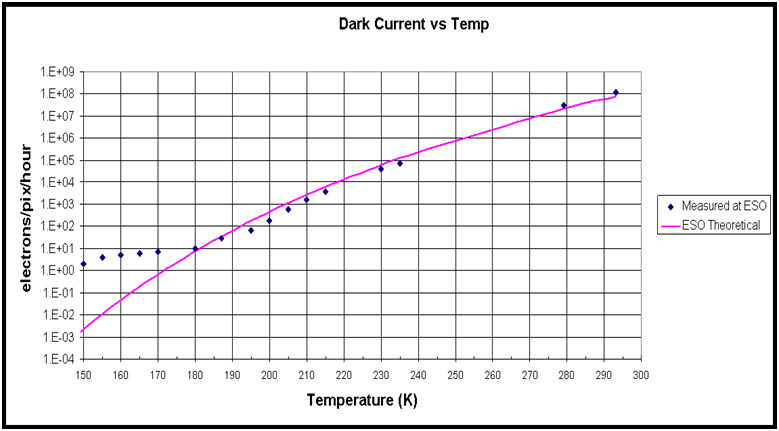
\includegraphics[width=0.7\textwidth]{../Images/Dark.png}
			\caption{Figure 1}\label{fig:dark_current}
		\end{figure}

		Figure 1 shows that relationship between temperature and dark current for a custom designed CCD provided to the European Southern Observatory and shows clearly the increase in dark current at higher temperatures. CCD’s are therefore cooled, often with the use of liquid nitrogen, to minimise this effect. The dark current itself is a relatively small electric current that flows through numerous photosensitive devices, and is one of the main sources of noise for a CCD.
	% subsubsection dark_current (end)

	\subsubsection{Sky Background} % (fold)
	\label{ssub:sky_background}
		The sky background is the incoming light from the sky measured on the telescope that is not from the source being observed. The amount of sky background can vary at different wavelengths and is mainly due to light diffusion by the atmosphere. There are numerous sources that contribute towards the sky background such as airglow and zodiacal light. Airglow is the atmospheric emission of photons at wavelengths from the near-UV to the near-IR range due to chemical reactions in the upper atmosphere\cite[page~9]{atmospheric_radiation_model}. These chemical reactions lead to light emission due to the decay of electrons from an excited state in one of the reaction products. One such example is the emission in the near infrared region by OH radicals created from a reaction between ozone and hydrogen in the upper atmosphere\cite{residual_OH_emission}. Other processes contributing to airglow are the recombination of ions originally ionised by the sun, and the luminescence of cosmic rays striking the upper atmosphere. Thermal radiation in the atmosphere by greenhouse gases also contributes to the sky background and is due to the absorption and emission of radiation from the Sun into the atmosphere in the mid-IR region. In this case, observations in the mid- and far-IR region must be carried out from outside the atmosphere\cite[pages~22--23]{Peter_Schneider_IR}. The sky background is therefore primarily an issue for ground based telescopes as they can incur a large background number of photons compared to the number of photons arriving from the source being observed. As space based telescopes are situated outside of the atmosphere, they avoid almost all of this background.
	% subsubsection sky_background (end)
% section observation_times (end)


    %!TEX root = mainfile.tex

\subsection{Dithering} % (fold)
\label{sub:dithering}
	Dithering is a technique used in photometry whereby the pointing is adjusted a small amount between exposures. This technique’s primary use it to account for dead pixels in the CCD; with adjustments of a few pixels the median stacking of the images means that any such defects will disappear. The technique also compensates for the presence of cosmic rays as well as undersampled images; where the sampling frequency is less than twice the highest frequency in the signal (Nyquist Theorem). Dithering also has the benefit of randomising the quantization error that occurs during the analogue-digital conversion of the signal [ADC_Kamensky]. Using a digital image processing method called ‘DRIZZLE’, originally developed for use in the Hubble Deep Field, the dithered images can be combined to produce more accurate observations for a given S/N [DRIZZLE].
% subsection dithering (end)


    \section{Telescopes Chosen for Investigation} % (fold)
    \label{sec:telescopes_chosen_for_investigation}
        %!TEX root = mainfile.tex

\section{The Hubble Space Telescope} % (fold)
\label{sec:the_hubble_space_telescope}

	\subsection{Mission Launch} % (fold)
	\label{ssub:mission_launch}
		On April 24th 1990 NASA’s Space Shuttle Discovery launched the world’s first space-based optical telescope; The Hubble Space Telescope (HST), named in honour of American astronomer Edwin P. Hubble. Edwin Hubble’s greatest contribution to astronomy was the Hubble Law which states that galaxies are receding from us at a speed directly proportional to their distance from us. This showed that our universe is expanding, a notion which underpins modern cosmological thinking. The telescope sits in a low-Earth orbit, as shown in figure~\ref{fig:hubble_space_telescope}, at an altitude of 569 kilometres completing one orbit of the Earth every 97\,minutes\cite{Hubsite_1}.
		\begin{figure}[ht]
			\centering
			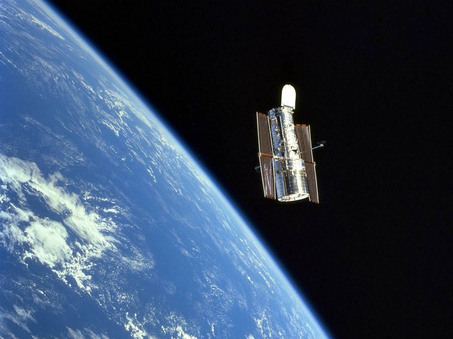
\includegraphics[width=0.5\textwidth]{../Images/Hubble_Space_Telescope.jpg}
			\caption{Photograph of HST orbiting the Earth.\label{fig:hubble_space_telescope}}
		\end{figure}

		The HST was designed to provide clear and deep views of distant galaxies and stars and most of the planets in our solar system. Hubble's domain extends from the ultraviolet through the visible and into the near-infrared\cite{NASA_1}.
	% subsection mission_launch (end)

	\subsection{Achievements to Date} % (fold)
	\label{ssub:achievements_to_date}
		The HST has provided unprecedented detail in images of star formation allowing astronomers to see the jets and disks present during the birth of new stars. It has also been able to study the atmospheric composition of extra-solar planets and take the first visible light picture of a planet outside our solar system; Fomalhaut b\cite{Hubsite_3}.

		Many EoR galaxies and candidate galaxies have been identified using HST data. In December 1995 the HST was pointed at what was believed to be a fairly empty and uninteresting patch of sky; 342 separate exposures were taken over 10 consecutive days and formed an image called the Hubble Deep Field (HDF)\cite{ESA_2}. The image contains around 3,000 objects of which the vast majority are galaxies, with a few local stars in the foreground. The HDF is one of the most iconic images of the 20th century, and it has since been cited in over 800 scientific papers.

		In 2004 its successor was revealed, the Hubble Ultra Deep Field (UDF); a million-second exposure in a 200\si{\arcsecond}$\times$200\si{\arcsecond} area of sky containing \num{10000} galaxies stretching back 13\,billion years\cite{Hubsite_2}. This exposure utilised the recently installed Advanced Camera for Surveys (ACS), seen in figure~\ref{fig:HUDF}. This survey was further refined in September 2012 in the Hubble eXtreme Deep Field (XDF) which utilised the recently installed WFC3 camera as well as combining over \num{2000} separate exposures from different sources\cite{ESA_2}.
		\begin{figure}[ht]
			\centering
			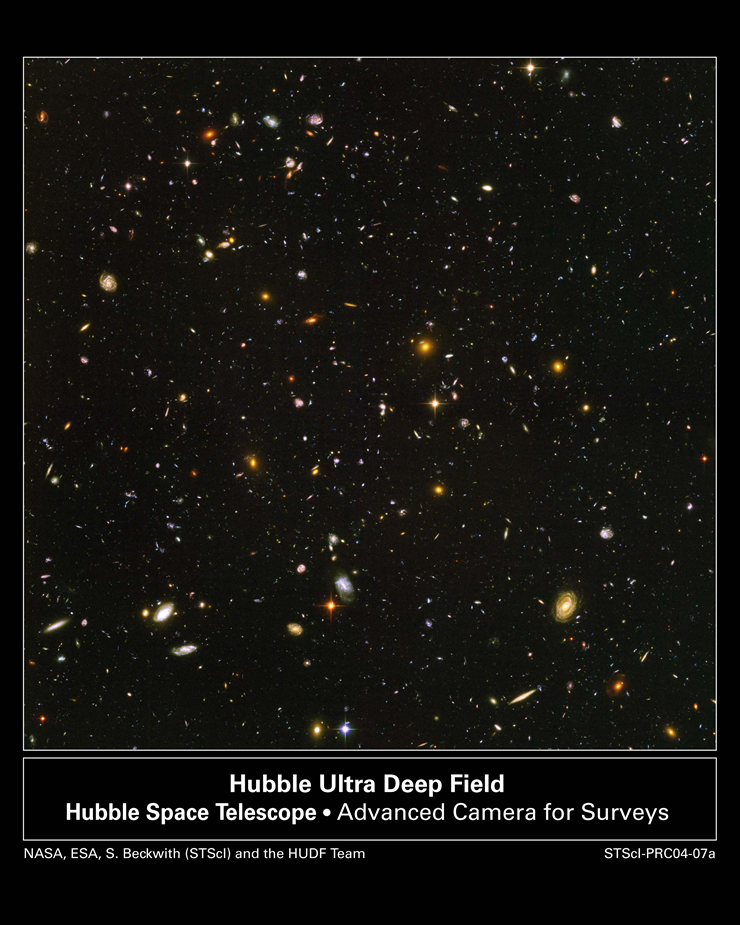
\includegraphics[width=0.8\textwidth]{../Images/HUDF.png}
			\caption{The HUbble Ultra Deep Field.\label{fig:HUDF}}
		\end{figure}

		Using data from the HUDF, object UDFj-39546284 was identified. In a paper by Bouwens et al, published in 2012, their best fit places it at a redshift of $11.8\pm0.3$\cite{Bouwens2012}. This would classify it as the oldest object ever observed. The exact nature of the object is not known but it is believed to be a mini-galaxy. Confirmation will require spectroscopic analysis, which is likely to be carried out by the James Webb Space Telescope. This observation demonstrates both the achievements and limits of the current technology.
	% subsection achievements_to_date (end)

	\subsection{Operation} % (fold)
	\label{ssub:operation}
		The HST is operated remotely from the earth, it has 4 antennae which can send and receive signals from the Flight Operations Team at Goddard Space Flight Centre in Greenbelt, Maryland via the Tracking and Data Relay Satellite system. For communication to be possible HST must have a direct line of sight to at least one of these 5 satellites.

		The HST is powered using 2 arrays of solar panels each capable of converting the Sun’s rays into \num{2800} watts of electricity. The arrays are able to store the electricity in batteries allowing the HST to remain active while in the Earth’s shadow (approximately 36\,minutes out of every 97\,minute orbit).

		Orbiting the Earth subjects the HST to extreme conditions due to the effect of zero gravity and the variation in temperature (up to around \SI{40}{\kelvin}) during each orbit. The optical system is held together using a skeleton (truss) constructed from Graphite epoxy. Graphite epoxy, commonly found in racquets and golf clubs is a stiff and lightweight material able to resist expansion and contraction due to temperature changes\cite{Hubsite_4}.
	% subsection operation (end)

	\subsection{Performance and Optical Telescope Array} % (fold)
	\label{ssub:performance_and_optical_telescope_array}
		The HST is constructed using a Ritchey-Chretien Cassegrain design; this allows high-performance over a wide field of view. The incoming light enters a tube with baffles removing any unwanted stray light, as shown in figure~\ref{fig:HST_optical_diagram} below. The light is then collected by the concave Primary mirror and reflected towards the smaller convex Secondary mirror. This light is then reflected back through a hole in the centre of the Primary mirror where it is focused onto a small area to be picked up by the instruments\cite{Hubsite_5}.
		\begin{figure}[ht]
			\centering
			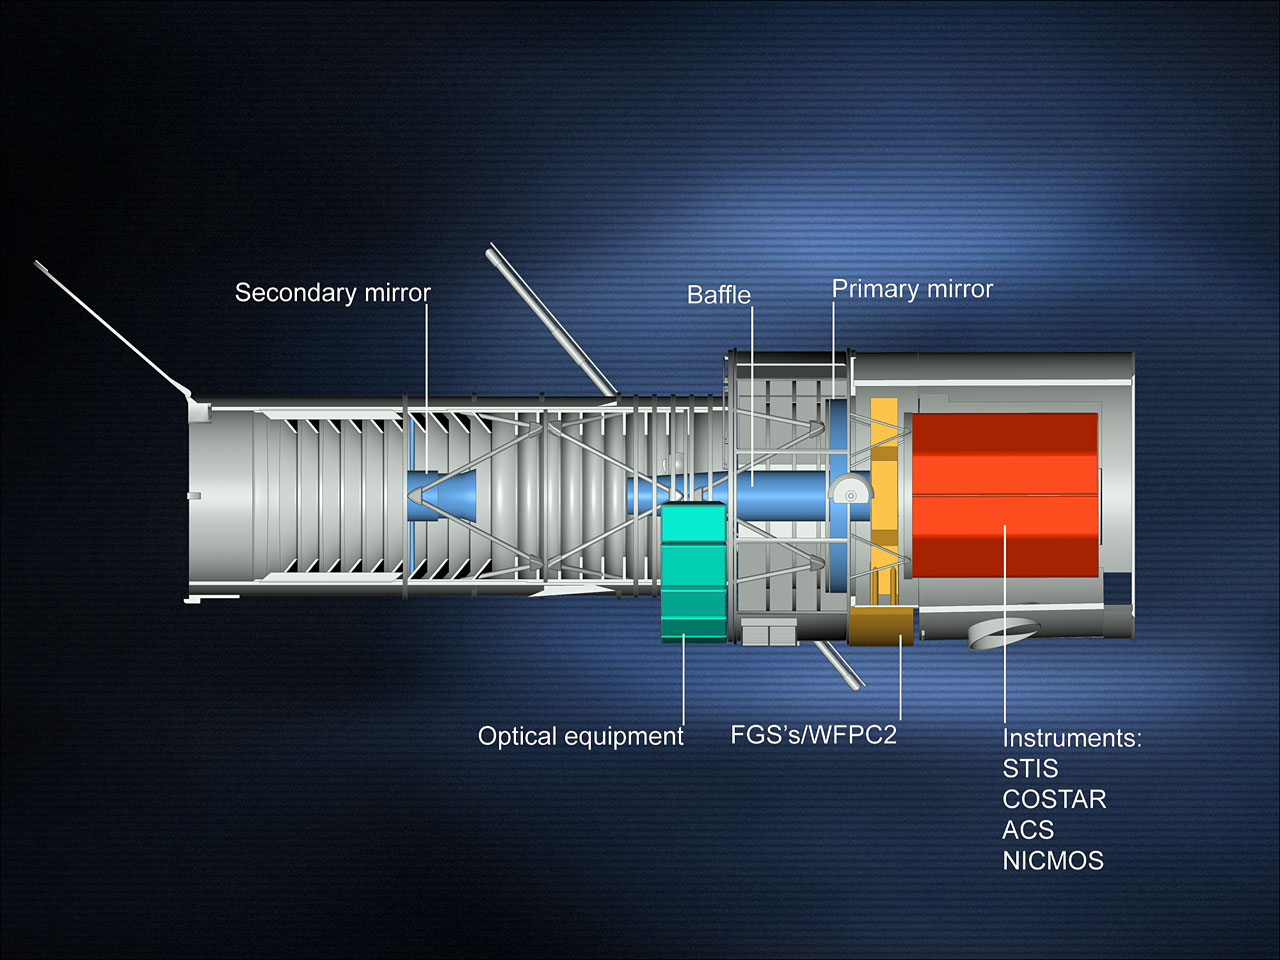
\includegraphics[width=0.5\textwidth]{../Images/HST_optical_diagram.jpg}
			\caption{Diagram showing basic systems of HST, note that WFC2 has since been replaced by WFC3.\label{fig:HST_optical_diagram}}
		\end{figure}

		The mirrors have been polished to an accuracy of better than the wavelength of visible light. When the HST was first launched the scientists soon realised that the curve to which the mirrors had been ground was not correct resulting in an error known as spherical aberration which blurred the images. A servicing mission in December 1993 deployed 5 pairs of mirrors which were able to successfully correct the error and allow Hubble to take the images it was intended to\cite{ESA_1}.

		There have been 4 servicing missions sent to the HST with the final mission taking place in May 2009. Over its lifetime the cameras and instruments have undergone many improvements and replacements. The camera currently operating that is of interest to this project is the WFC3/IR camera, installed in 2009. This camera is able to observe in the near-infra-red where we expect to see the Lyman-break galaxies. Table~\ref{tab:HST_technical} shows the key technical data for the HST, amazingly the HST is so precise it is able to lock onto a target at a distance of 1 mile without deviating more than the width of a human hair.
		\begin{table}[ht]
			\begin{center}
				\begin{tabular}{l|l}
					Component	& 	Details \\
					\hline\hline
					Primary Mirror Diameter & \SI{2.4}{\metre} \\ \hline
					Secondary Mirror Diameter & \SI{0.3}{\metre} \\ \hline
					Wavelength range & 800--1700\si{\nano\metre} \\ \hline
					Total Field of View & \SI{123}{\arcsecond}$\times$\SI{136}{\arcsecond} (\SI{16728}{\arcsecond}$^2$) \\ \hline
					Pixel Size & $18\times18$\,\si{\micro\metre} \\ \hline
					Plate Scale & \SI{0.13}{\arcsecond\per\pixel} \\ \hline
					\multirow{3}{*}{Quantum Efficiency} & 77\% at \SI{1000}{\nano\metre}\\
					 & 79\% at \SI{1400}{\nano\metre}\\
					 & 79\% at \SI{1650}{\nano\metre}\\ \hline
					Dark count &  \SI{0.048}{\electron\per\second\per\pixel} \\ \hline
					Readout noise & \SI{12.0}{\electron\per\second\per\pixel} \\ \hline
					Full Well & \SI{77900}{\electron} \\ \hline
					Gain & 2.28--2.47\si{\electron\per\ADU} \\ \hline
					Operating Temperature & \SI{145}{\kelvin} \\ \hline
					FWHM & \SI{0.151}{\arcminute} at \SI{1600}{\nano\metre}
				\end{tabular}
			\end{center}
			\caption{Technical data for HST WFC3/IR camera system\cite{WFC3_IHB}}
		\label{tab:HST_technical}
		\end{table}
	% subsection performance_and_optical_telescope_array (end)

% section the_hubble_space_telescope (end)

        %!TEX root = mainfile.tex

\subsection{Spitzer Space Telescope} % (fold)
\label{sub:spitzer_space_telescope}
(Dorothy with contributions from Catherine)

	Spitzer Space telescope was launched by NASA on 25th August 2003\cite{fast_facts_spitzer} and is designed for use in the infrared. It was the last of NASA's ``Great Observatories'', working alongside HST in the optical, Compton Gamma Ray Observatory and Chandra X-ray Observatory. The telescope is \SI{85}{\centi\metre} in diameter, and sits in an Earth-trailing orbit around the Sun, shown in Figure~\ref{fig:spitzer_orbit_LARGE}. It is a Cassegrain telescope, meaning it has primary and secondary hyperbolic mirrors to focus the light and reduce spherical aberration, in a similar manner to Hubble. The majority of Spitzer's instrumentation is now non-operational due to a lack of cryogen, but some photometry remains possible.
	\begin{figure}[htbp]
		\centering
		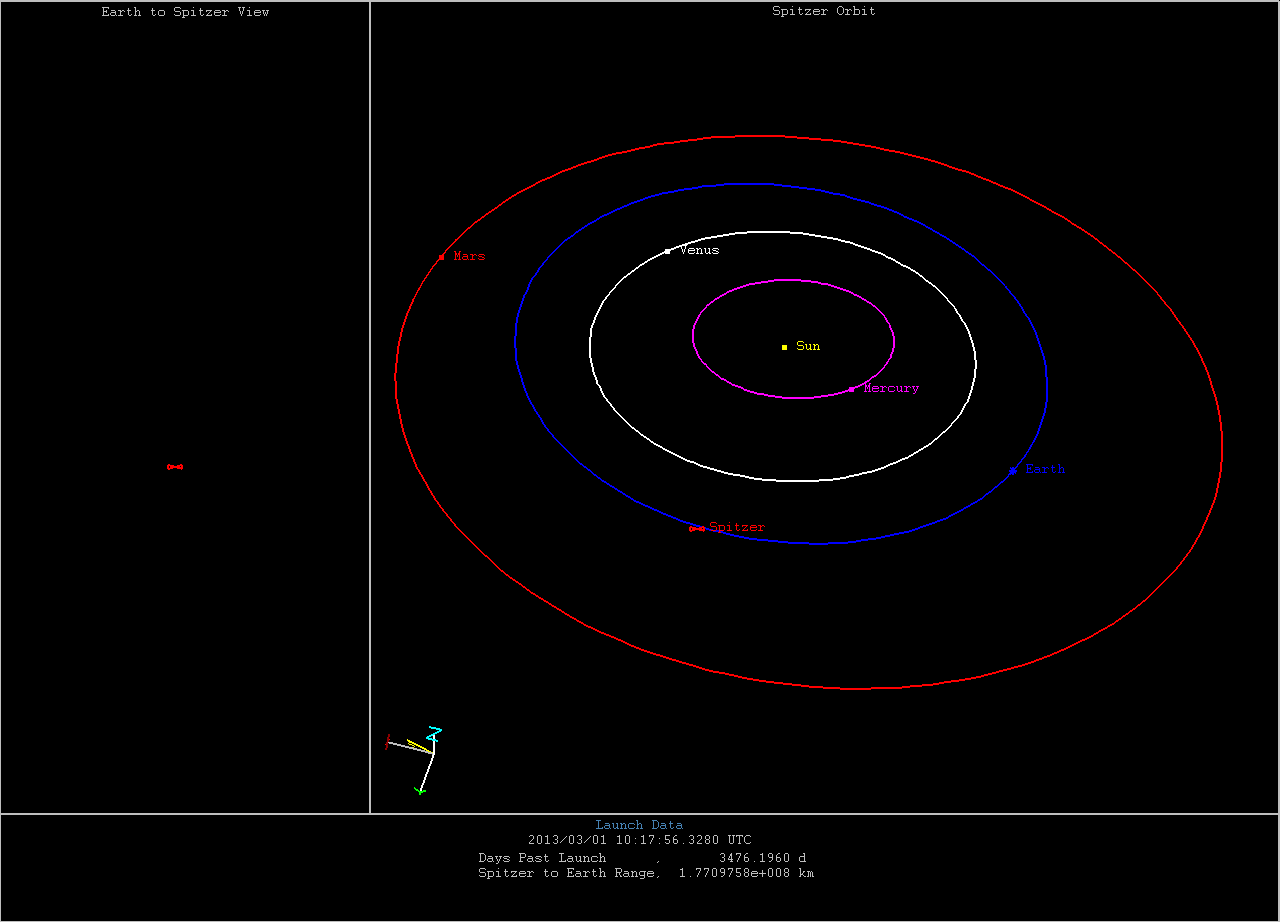
\includegraphics[trim = 110mm 70mm 5mm 30mm, clip, width=0.6\textwidth]{../Images/spitzer_orbit_LARGE.png}
		\caption{The Spitzer Space Telescope's Orbit\cite{where_is_spitzer}.\label{fig:spitzer_orbit_LARGE}}
	\end{figure}

	\subsubsection{Capabilities} % (fold)
	\label{ssub:spitzer_capabilities}
		Spitzer had the capabilities detailed in Table~\ref{tab:Spitzer_cababilities}.
		\begin{table}[htbp]
			\begin{center}
				\begin{tabular}{l|l}
					Component   &   Wavelength Range \\
					\hline\hline
					Imaging/Photometry & 3--180\si{\micro\metre} \\
					Spectroscopy       & 5--40\si{\micro\metre} \\
					Spectrophotometry  & 50--100\si{\micro\metre}
				\end{tabular}
			\end{center}
			\caption{Details of instrumentation for Spitzer\cite{WFC3_IHB}.\label{tab:Spitzer_cababilities}}
		\end{table}

		It employed three scientific instruments which helped it do the above:
		\begin{itemize}
			\item Infrared Array Camera (IRAC): an imaging camera working in the near IR at wavelengths of 3.6, 4.5, 5.8 and 8\,micrometres.
			\item Infrared Spectrograph (IRS): performing spectroscopy from 5 to 40\,micrometres.
			\item Multiband Imaging Photometer (MIPS): detected wavelengths in the far IR, at 24, 70 and 160\,micrometres.
		\end{itemize}

		The telescope was cryogenically cooled to around \SI{1.4}{\kelvin}, allowing all the instruments to function without excessive thermal interference from the telescope itself. The mission, labelled the `Cold Mission', was estimated to last between 2 and 5 years, depending on when the cryogen ran out. During this time, Spitzer imaged in all four NIR filters simultaneously, as well as doing spectroscopy, and some imaging in the far infrared. In 2009, when the cryogen ran out, the longer wavelength filters became non-operational, and the Spitzer `Warm Mission' continued imaging with the nearest IR filters ($3.6$ and $4.5$\,micrometres). This was made possible because Spitzer's orbit keeps it substantially cooler than an Earth-centred orbit would, due to the lack of IR radiation received from Earth. Furthermore it is made mostly of beryllium which has a low heat capacity at low temperatures, helping to keep it cool.

		In order to keep enough sunlight on the solar panels, Spitzer cannot point further than 120\,degrees away from the Sun. However, it also cannot get closer than 80\,degrees towards the Sun in case damage is done to the scientific instruments. This is a limitation on the area of sky which can be observed, meaning that some regions can only be seen for 40 days semi-annually, whilst other areas can be observed all year round.

		The spectrograph (IRS) operated at wavelengths too long to be of use to study the EoR, as did the far IR photometry (MIPS), however the near IR photometry capabilities of both the Spitzer warm and cold missions have been used to study high redshift galaxies, and in conjunction with HST have confirmed galaxies at redshifts as far back as $z\approx10$. Particularly the 3.6 and 4.5\,micrometre filters observe significant flux from such galaxies, and so these have been used in a number of studies looking for high redshift galaxies.
	% subsubsection capabilities (end)

	\subsubsection{Studies involving Spitzer} % (fold)
	\label{ssub:studies_involving_spitzer}
		Coe et al (2012)\cite{0004-637X-762-1-32} reports a $z\approx11$ candidate which had been observed using HST (WFC3, ACS) and Spitzer (IRAC) for longer wavelengths. This is one of the highest redshift candidates to date. The Spitzer data was taken over a total integration time of 5 hours.

		An earlier study in 2008 by Richard et al also used Hubble to detect galaxies greater than redshift seven (making use of gravitational lenses). Spitzer imaged these galaxies to help confirm that they were not foreground objects of a different nature, by looking at the flux in longer wavelength filters\cite{0004-637X-685-2-705}.

		In 2005, during the cold mission, a study was made by Spitzer on a confirmed $z=6.56$ galaxy (HCM 6A) lensed by a cluster (Abell 370). The study was used to detect the rest frame optical emission of this galaxy in order to better understand the physical properties of objects at such high redshifts\cite{1538-4357-635-1-L5}. Several other papers have also used Spitzer data in the study of high redshift galaxies.

		Spitzer also has ideal filters to look at the Balmer or \SI{4000}{\angstrom} break which, if prominent, would indicate an older stellar population and suggest that the object is more likely a contaminant than a high redshift LBG, since high redshift LBGs do not contain many old stars.

		The data in Table~\ref{tab:Spitzer_technical} shows some of the key technical data availible for the telescope.
		\begin{table}[htbp]
			\begin{center}
				\begin{tabular}{l|l}
					Component   &   Details \\
					\hline\hline
					Primary mirror & \SI{0.85}{\metre} \\
					FoV & \SI{5.2}{\arcminute}$\times$\SI{5.2}{\arcminute} \\
					Pixel size & \SI{1.2}{\arcsecond}$\times$\SI{1.2}{\arcsecond} \\
					Detector Array & $256\times256$\,\si{\pixel} \\
					\multirow{2}{*}{Full well} & 145,000 at \SI{3.6}{\micro\metre} \\
							& 140,000 at \SI{4.5}{\micro\metre} \\
				\end{tabular}
			\end{center}
			\caption{Technical data for Spitzer\cite{Spitzer_Heritage_Archive_Documentation}.\label{tab:Spitzer_technical}}
		\end{table}
	% subsubsection studies_involving_spitzer (end)
% subsection spitzer_space_telescope (end)

        %!TEX root = mainfile.tex

\subsection{Euclid} % (fold)
\label{sub:euclid}

	\subsubsection{Mission Overview} % (fold)
	\label{ssub:mission_overview}
		The Euclid mission is planned for launch in 2020, at an estimated total cost of 800\,million Euros\cite{bbc_euclid}. Its primary goal is to conduct a wide survey; some 15000 degrees of sky is planned to be covered. There is also to be a deep survey which is expected to cover around 40 degrees to a depth 2 magnitudes deeper than the wide survey. It will have a near infra-red camera and spectrometer as well as an optical camera. The primary mission  objectives are expected to be completed within 7 years. One of Euclid’s main scientific objectives with the deep field is to study high redshift galaxies at z =6+ over a very wide survey area. This will give astronomers the opportunity to spectroscopically confirm hundreds of galaxies for use in the study of the EoR. It will help constrain the bright end of the luminosity function at high z.
	% subsubsection mission_overview (end)

	\subsubsection{Capabilities} % (fold)
	\label{ssub:capabilities}
		\begin{itemize}
			\item Visual Imaging/ Photometry, 550--900\si{\nano\metre}
			\item Spectroscopy, 1100--2000\si{\nano\metre}
			\item NIR Imaging/ Photometry, 920--2000\si{\nano\metre} (Y, J,H bands)
		\end{itemize}

		Euclid will have two instruments in order to do the above; a wide-band imaging system in the visible (VIS), and an instrument capable of both slit-less spectroscopy as well as NIR imaging. These instruments will be operated simultaneously.
	% subsubsection capabilities (end)

	\subsubsection{Key Technical Data} % (fold)
	\label{ssub:key_technical_data}
		The data in table~\ref{tab:Euclid_technical} is quoted for the deep survey NIR photometry. Some data is subject to slight change as the planning stages progress.
		\begin{table}[ht]
			\begin{center}
				\begin{tabular}{l|l}
					Component & Details \\
					\hline\hline
					Primary mirror		& \SI{1.2}{\metre} \\ \hline
					FoV 				& $0.763\times0.763$\si{\degree\squared} \\ \hline
					Pixel size			& \SI{0.3}{\arcsecond}$\times$\SI{0.3}{\arcsecond} \\ \hline
					Detector Array		& \num{2000}$\times$\num{2000}\,\si{\pixel} \\ \hline
					Resolution 			& 0.3 to \SI{0.6}{\arcsecond} (in J band) \\ \hline
					Plate Scale (infra-red)	& \SI{0.3}{\arcsecond\per\pixel}
				\end{tabular}
			\end{center}
			\caption{Technical data for HST WFC3/IR camera system\cite{WFC3_IHB}.\label{tab:Euclid_technical}}
		\end{table}
	% subsubsection key_technical_data (end)
% subsection euclid (end)

        %!TEX root = mainfile.tex

\subsection{European Extremely Large Telescope} % (fold)
\label{sub:european_extremely_large_telescope}
	One of a new generation of ground based telescopes, the European Extremely Large Telescope (E-ELT), shown in figure~\ref{fig:artist_eelt}, is scheduled for first light in 2022 and has a projected lifetime of 30 years, although major upgrades are expected during this period\cite[p.~163]{E_ELT_Construction_Proposal}, and an estimated cost of around 1083\,million Euros. The Telescope will be constructed on Cerro Armazones in Chile at an altitude of approximately \SI{3060}{\metre} and will be part of the La Silla Paranal observatory. With a primary mirror diameter of \SI{39.9}{\metre}, the E-ELT will be the largest optical/near-infrared telescope in the world. The telescope will also incorporate adaptive optics, discussed in section~\ref{ssub:adaptive_optics}, which will result in it being able to correct for atmospheric perturbations and therefore be diffraction limited.
	\begin{figure}[!htb]
		\centering
		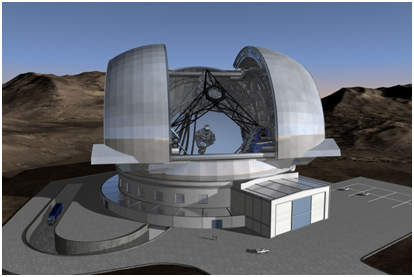
\includegraphics[width=0.6\textwidth]{../Images/E-ELT.png}
		\caption{An artist's impression of the E-ELT\cite{E_ELT_Enclosure}}\label{fig:artist_eelt}
	\end{figure}

	One of the most important components of the E-ELT is the dome within which the telescope is enclosed. This primarily provides protection to the telescope against unfavourable weather conditions and during the day. The dome is designed to allow complete freedom to the telescope, allowing it to position itself, permitting observations between a $20^{\circ}$ angle to the horizon and zenith and also incorporates a windscreen protecting the mirrors. As well as being water-tight, the dome is also air-tight to minimise the air-conditioning load. The E-ELT will use an air-conditioning system to cool the mirror and instrumentation to ensure optimum operating conditions in preparation for the upcoming night.

	The E-ELT utilises a three mirror anastigmat system with two further mirrors providing the adaptive optics, shown below in figure~\ref{fig:5_mirror_eelt}, with the fifth mirror directing the beam towards the Nasmyth focus\cite[p.~16]{E_ELT_Construction_Proposal}. The primary mirror, measuring \SI{39.3}{\metre} in diameter, will be comprised of 798 hexagonal segments eventually producing a collecting area of \SI{978}{\square\metre}. The E-ELT will therefore have a light collecting power approximately 13 times larger than any existing telescope and is predicted to produce images 16 times sharper than those of the Hubble Space Telescope. Other new generation extremely large telescopes include the Giant Magellan Telescope with a primary mirror of diameter \SI{25}{\metre} and the Thirty Metre Telescope with a primary mirror of diameter \SI{30}{\metre}. The E-ELT however remains the largest of these planned telescopes.
	\begin{figure}[!htb]
		\centering
		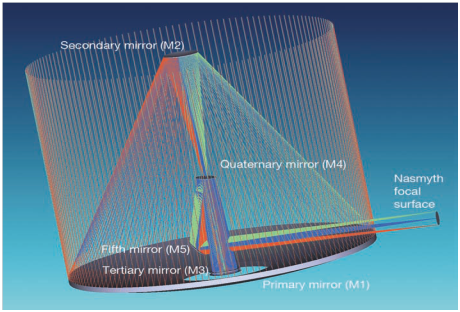
\includegraphics[width=0.6\textwidth]{../Images/Anastigmat.png}
		\caption{The 5 mirror design to be utilised on the E-ELT}\label{fig:5_mirror_eelt}
	\end{figure}

	\subsubsection{Main Aims} % (fold)
	\label{ssub:main_aims}
		One of the main aims of the E-ELT will be the search for extra-solar planets.  This will include the detection of extra-solar planets using the radial velocity technique, the detection of variations of the radial velocity of a star with respect to the Earth in response to the gravity of an orbiting planet, as well as possible direct imaging of larger planets. The E-ELT may also be used to characterise the atmosphere of these larger planets using low resolution spectroscopy. The observation of giant planets in star forming regions and young stellar clusters will also provide an insight into their evolution.

		Another of the main aims is the study of the universe at high redshift. The E-ELT will look back at the earliest galaxies formed after the ``dark ages'', the galaxies therefore responsible for the re-ionisation of the universe. Properties of these early galaxies including their star formation rates, ages, metallicities and stellar masses will be determined contributing to a better understanding of galaxy formation and evolution.

		The E-ELT will also help to understand the nature of dark energy through the discovery and identification of type 1a supernovae. As these are excellent distance indicators, they can be used to map space and its expansion history thus providing information on what is believed to be the source of this expansion. The E-ELT will also attempt to measure small time-drifts in the redshifts of distant objects in the intergalactic medium, a consequence of the evolution the universal expansion rate. The E-ELT will also attempt to discover variations of physical constants over time which, if found to be the case, will have great consequences on our understanding of the general laws of physics.
	% subsubsection main_aims (end)

	\subsubsection{Instrumentation} % (fold)
	\label{ssub:instrumentation}
		At first light, the E-ELT will have just two instruments\cite{E_ELT_Instrumentation}, a diffraction-limited near-infrared imager (MICADO) as well as a single-field near-infrared wide-band integral field spectrograph (HARMONI). Three further objects, a mid-infrared imager and spectrometer (METIS), a high-resolution spectrometer (SIMPLE) and multi-object spectrometer (OPTIMOS) will be added soon after first light\cite{E_ELT_Instrumentation}. There are also some other concepts being studied for use on the E-ELT including a planet imager with extreme adaptive optics (EPICS). Importantly, the instrumentation available will mean that the E-ELT can be used for both photometry and spectroscopy and is also said to be able to switch between these instruments in a matter of minutes.
	% subsubsection instrumentation (end)
% subsection european_extremely_large_telescope (end)

        %!TEX root = mainfile.tex

\subsection{James Webb Space Telescope} % (fold)
\label{sub:james_webb_space_telescope}
	The James Webb Space Telescope (JWST) is a near-infrared space based telescope. Formerly known as the Next Generation Space Telescope, it was renamed after the NASA administrator James Edwin Webb in 2002. It is an international collaboration between NASA, the European Space Agency (ESA) and the Canadian Space Agency (CSA). The JWST’s capabilities will enable a broad range of investigations across many different fields in astronomy. However, its primary goal is to observe the most distant objects in our universe that are beyond the reach of any current ground or spaced based instruments. More importantly for our specific goals it will enable the study of the epoch of re-ionisation and the first stars\cite{primary_mirror_construction}.

	The JWST consists of four main instrument components:
	\begin{itemize}
		\item Near-Infrared Camera (NIRCam),
		\item Near-Infrared Spectrograph (NIRSpec),
		\item Mid-Infrared Instrument,
		\item Fine Guidance Sensor.
	\end{itemize}

	NIRCam uses a technique of CCD photometry to measure the magnitude of high redshift galaxies. It consists of ten mercury-cadmium-telluride (HgCdTe) detector arrays which are analogous to CCD’s found in digital cameras. Coronagraphs enable NIRCam to collate images of very faint objects around a central bright object\cite{primary_mirror_construction}.

	NIRSpec enables the JWST to obtain the spectrums of high redshift galaxies. It is comprised of micro shutter array with \num{62000} shutters that can be closed and opened individually meaning that the JWST can record the spectrums of one hundred different objects simultaneously. The device will have a total field of view of $3\times3$ arcminutes. As well as the micro shutter array NIRSpec will also have five fixed slits for high constant spectroscopy. There is an integral field unit spectrograph (IFU) with thirty slicers meaning that the spectrums of extended bodies can be found. The wavelength range over which NIRSpec can successfully operate is \SI{0.6}{\micro\metre} to \SI{5}{\micro\metre}\cite{primary_mirror_construction}.

	The Mid-Infrared Instrument will be used to obtain the spectrums of objects similar to NIRSpec. However the range over which it will operate will be \SI{5}{\micro\metre} to \SI{29}{\micro\metre}\cite{primary_mirror_construction}.

	Fine Guidance sensor (FGS) is a sensitive camera that will provide critical information for the JWST’s altitude control system. Its main functions include obtaining images for target acquisition and providing guide stars for the alignment and phasing for the segments of the primary mirror\cite{stsci_edu}.

	The JWST’s primary advantage over other current (and planned) space telescopes is its large primary mirror which has a diameter of 6.5\,metres. The next largest mirror of any spaced based telescope belongs to the Hubble Space Telescope (HST) which has a diameter of 2.4\,metres. JWST’s primary mirror is fabricated from eighteen beryllium segments each with a diameter 1.3\,metres which when correctly phased together act as a single mirror. The mirror phasing is achieved due to the fact that every segment has six degrees of rotational freedom by way actuators attached to their underside and the back plane. The back plane holds the primary mirror structure together\cite[p.~568--569]{gardner2006james}.
	\begin{figure}[!htbp]
		\centering
			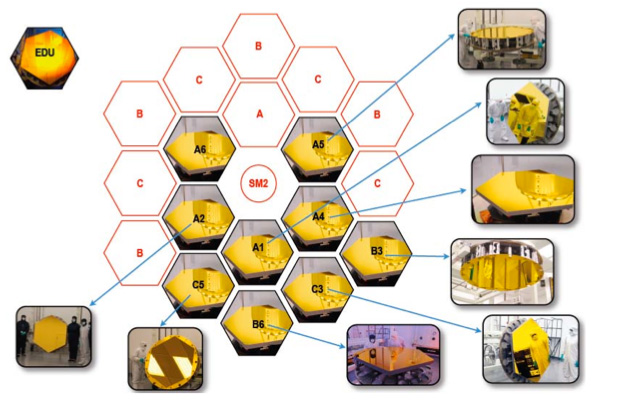
\includegraphics[width=0.6\textwidth]{../Images/JWST_mirror_construction.jpeg}
		\caption{\cite{primary_mirror_construction}\label{fig:james_web_layout}}
	\end{figure}

	The adjustability of JWST’s primary mirror allows for active optics, as discussed in Section~\ref{ssub:adaptive_optics}. When a mirror of this size pivots to look at different portions of space it naturally bends and deforms. By focusing on a reference object this deformity can be constantly corrected using the actuators connected to each segment of the primary mirror. It will be coated in gold to ensure a maximum reflectivity of 98\%\cite{mtwilson}.

	The Orbit of the JWST will lie at the second Lagrange point (L2) \SI{150000}{\kilo\metre} from Earth. L2 is one of five solutions to the three body problem posed by Joseph Louie Lagrange. It means that when the JWST is in orbit, the sun moon and earth will all stay in the same position relative to each other. The orbit is slightly inclined with respect to the elliptical plane, avoiding moon and earth eclipses of the sun, thus ensuring continuous electrical power is supplied. Orbit shown below in figure~\ref{fig:james_web_orbit}\cite{primary_mirror_construction}.
	\begin{figure}[!htbp]
		\centering
			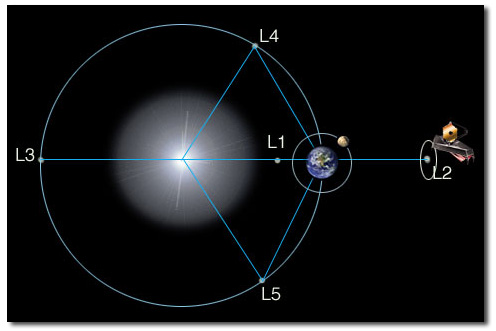
\includegraphics[width=0.5\textwidth]{../Images/JWST_orbit_L2.jpeg}
		\caption{Diagram of the orbit of the James Webb Space Telescope\label{fig:james_web_orbit}}
	\end{figure}

	The JWST is fitted with a sunshield which reduces the incident radiation of approximately 200 KW to a few milliwatts. This solar attenuation is achieved through the five layer design of the sunshield. Each layer is separated from the next via a vacuum which allows for passive cooling of the JWST. The sunshield will a surface area of approximately \SI{250}{\square\metre} which is too large to fit inside any current spacecraft so will be unfolded into position once the JWST is in orbit at L2. Due to this size, solar radiation will cause a build-up of angular momentum throughout its service. This will be offset by firing service thrusters used primarily for obit maintenance.

	The JWST is a three mirror anastigmat meaning it can minimize the three main optical aberrations, namely; spherical aberration, coma and astigmatism. The effective focal length of the mirrors combined is \SI{131.4}{\metre}. The basic layout can be seen in Figure~\ref{fig:james_web_layout}.

	For the most part the JWST will be background limited as opposed to diffraction limited. The background is due mostly to scattered zodiacal light, scattered starlight and thermal emission from the sunshield. The background due to these factors can be seen in Table~\ref{tab:JW_exposure_times_for_galaxies}. The imaging performance of the JWST will be diffraction limited (i.e.\ limited by the optical power of the telescope) at \SI{2}{\micro\metre} with a Strehl ratio greater than 0.80.

	The field of view refers to the fraction of the celestial sphere that the telescope can point at any given moment. The main limitation to the JWST’s field of view is the sunshield means that only 31\% of the sky can be seen for more than 197\,days. All regions of sky have at least 51\,days of continuous visibility per year\cite[p.~561--572]{gardner2006james}.

	Table~\ref{tab:JW_exposure_times_for_galaxies} below shows the information required in order to calculate exposure times for galaxies of given red shifts and magnitudes at a set signal to noise ratio.
	\begin{table}[!htbp]
		\begin{center}
			\begin{tabular}{c|c}
				Read Noise 					& 10 \\
				Dark Current 				& \SI{0.018}{\electron\per\second\per\pixel} \\
				Diameter of Primary Mirror 	& \SI{8.2}{\metre} \\
				Quantum Efficiency 			& 0.8 \\
				Sky Background 				& 0.005\,photon s$^{-1}$pixel$^{-1}$) \\
				Gain 						& 1.8\si{e}ADU$^{-1}$) \\
				Mirror Reflectivity 		& 0.98 \\
				CCD Pixel Number 			& $2048 \times 2048$
			\end{tabular}
		\end{center}
		\caption{Information required in order to calculate exposure times for galaxies of given red shifts and magnitudes.\label{tab:JW_exposure_times_for_galaxies}}
	\end{table}
% subsection james_webb_space_telescope (end)

    % section telescopes_chosen_for_investigation (end)

    %!TEX root = mainfile.tex

\clearpage
\section{Determining the Observation Strategy} % (fold)
\label{sec:method_for_strategy_choosing}
	\subsection{Method for Determination} % (fold)
	\label{sub:method_for_determination}
	(Dorothy and Mike)

		A range of factors were considered when determining which telescope, survey area and survey depth were best suited to the mission of observing the EoR. Firstly, time was an overall constraint on observations, with the Hubble ultra-deep field setting a realistic upper limit of around \SI{2e6}{\second} for a total exposure time. The primary aim was to see a significant number of $z\ge6$ galaxies, but it was also considered that at very high redshift (i.e.\ greater than ten), the number density of visible objects would decrease rapidly, so there were diminishing returns when looking for candidates at increasingly high redshifts. The following procedure outlines the method by which the final photometry strategy was obtained.

		Firstly the prediction group's program was run for a large range of magnitudes and redshifts. The inputs were as shown in Table~\ref{tab:program_inputs}.
		\begin{table}[htbp]
			\begin{center}
				\begin{tabular}{c|c}
					Parameter 	& Input \\
					\hline \hline
					$z_1$ & 6 \\
					$z_2$ & 16 \\
					$D_z$ & 0.5 \\
					$M_1$ & 26 \\
					$M_1$ & 35 \\
					$D_m$ & 0.05 \\
					Shell number & 100 \\
					Bin number & 100
				\end{tabular}
			\end{center}
			\caption{Data highlighting which filters would be useful for observing particular redshift galaxies\cite{Galactic_Astronomy_Binney_Merrifield}\label{tab:program_inputs}}
		\end{table}

		This gave a large selection of number densities in ``bins'' which could be summed to give the total number density of objects within a redshift and magnitude range. The observational strategists were therefore in charge of choosing realistic limits for these two parameters.

		Either a magnitude limit was set directly, or, using the ``observation time'' spreadsheet, a time limit was imposed, which therefore put constraints on how deep each telescope could observe to. Time limits were primarily needed for those observations that were looking to see the highest redshift objects, and therefore benefited from very faint magnitudes and long total exposure times.

		Subsequently, all data upwards from the faintest magnitude was put into an excel spreadsheet where it could be summed to find the total number of galaxies given the constraints.

		When a total survey time was set, this allowed the observational strategists to quantitatively say what combination of survey area and survey depth yielded the highest number of galaxies within the required redshift range. A simplified example is given below:

		\paragraph{Example} % (fold)
		\label{par:example}
			For a particular telescope, the total exposure time constrains the magnitude. A set of data that demonstrates this is shown in Table~\ref{tab:dimmest_mag_observable}.
			\begin{table}[htbp]
				\begin{center}
					\begin{tabular}{c|>{\centering\arraybackslash}m{4cm}|>{\centering\arraybackslash}m{4cm}}
						Time (\SI{e6}{\second})& Dimmest Magnitude at that Depth & Number Density of Galaxies per degree \\
						\hline \hline
						1 & 32.1 & 5000 \\
						0.5 & 30.8 & 2600 \\
						0.25 & 29.6 & 1600 \\
					\end{tabular}
				\end{center}
				\caption{The limit of magnitude, and hence number of galaxies observable, for different observing times.\label{tab:dimmest_mag_observable}}
			\end{table}

			Subsequently, there are many possible ways to make up a total survey time of \SI{1e6}{\second}, as demonstrated in Table~\ref{tab:total_survey_time_breakdowns}. In this example, the largest number of galaxies can be observed by doing $4 \times (0.25\times 10^6)$\,\si{\second} exposures. However, this favours finding more galaxies at low redshift and fewer at the high end.
			\begin{table}[htbp]
				\begin{center}
					\begin{tabular}{c|>{\centering\arraybackslash}m{5cm}}
						Survey Makeup (\SI{e6}{\second}) & Number of Galaxies Expected per degree of Total Survey\\
						\hline \hline
						$1\times 1$ & 5000 \\
						$2\times 0.5$ & 5200 \\
						$4\times 0.25$ & 6400 \\
						$4\times 0.25$ + $1\times 0.5$ & 5800 \\
					\end{tabular}
				\end{center}
				\caption{Different ways of making up a total survey time of \SI{1e6}{\second}.\label{tab:total_survey_time_breakdowns}}
			\end{table}

		% paragraph example (end)
	% subsection method_for_determination (end)
% section method_for_strategy_choosing (end)

    %!TEX root = mainfile.tex

\subsection{Observing Strategy for Redshift 8.5--10} % (fold)
\label{sub:using_euclid_for_a_survey_of_edshift_8_54_to_10_1}
	Due to its large field of view, Euclid space telescope will be useful for studying a large number of galaxies, however it has been found to be limited by its filters to providing colour information only for those objects between redshift 8.5 and 10, Section~\ref{sec:Photometry_Colour}. The Euclid survey as described in Section~\ref{sub:euclid} is planned to take approximately six years, but this will only reach a magnitude of 26. It was investigated what galaxies the telescope would be able to observe if the magnitude limit was increased, and the results are shown in Table~\ref{tab:filters_for_particular_redshift_galaxies}.

	It must be noted that the program results predict different numbers of galaxies than the Euclid documentation. The prediction group's program is the data on which the following calculations are based. The survey method adopted for this project would also be different from that detailed by the Euclid ``red book''; rather than revisiting the same patch of sky infrequently, the aim would be to stare continuously at a particular point until the required depth was met. No wide survey is required for this project since the galaxies at the high redshifts being studied all have faint magnitudes. This will take a considerable length of time to see; hence a wide survey at such depths is implausible.

	Table~\ref{tab:filters_for_particular_redshift_galaxies} shows the number of galaxies observable for survey times of 0.1, 0.2, and 0.5\,million seconds. The number of galaxies that would be observed at different magnitudes is presented, and the table also displays the time taken for 1\,FoV, and the number of galaxies in that field of view for each magnitude. The red number indicates how many FoVs were possible given the set total observing time. N/A indicates that there were either no galaxies at this magnitude, or that the time taken to get to this magnitude was larger than the intended total survey time.
	\begin{table}[htbp]
		\begin{center}
			\begin{tabular}{c|c|c|c|c|c}
				\multirow{2}{*}{Magnitude}	&Time for	&Number of	&\multicolumn{3}{|c}{Galaxies in total observing time of:}\\
					\cline{4-6}
					&1\,FoV (\si{\second})	&galaxies in 1 FoV	&0.1 mil	&0.2 mil	&0.5 mil\\
				\hline \hline
				27		&\num{2.09e3}	&None	&N/A	&N/A	&N/A\\
				28		&\num{7.67e3}	&0.052	&0.6 (13)	&1.35 (26)	&3.38 (65)\\
				28.5	&\num{1.65e4}	&1.26	&7.56 (6)	&15.12 (12)	&37.8 (30)\\
				29		&\num{3.78e4}	&12.55	&25.1 (2)	&62.75 (5)	&163.15 (13)\\
				29.5	&\num{9.90e4}	&69.37	&69.37 (1)	&138.74 (2)	&346.85 (5)\\
				30		&\num{2.25e5}	&256.23	&N/A		&N/A		&512.46 (2)\\
				31		&\num{1.39e6}	&1653.35	&N/A	&N/A		&N/A
			\end{tabular}
		\end{center}
		\caption{Data highlighting which filters would be useful for observing particular redshift galaxies\cite{Galactic_Astronomy_Binney_Merrifield}}
		\label{tab:filters_for_particular_redshift_galaxies}
	\end{table}

	\begin{figure}[htbp]
		\centering
			\begingroup\endlinechar=-1
				\resizebox{0.8\textwidth}{!}{%
					% GNUPLOT: LaTeX picture with Postscript
\begingroup
  \makeatletter
  \providecommand\color[2][]{%
    \GenericError{(gnuplot) \space\space\space\@spaces}{%
      Package color not loaded in conjunction with
      terminal option `colourtext'%
    }{See the gnuplot documentation for explanation.%
    }{Either use 'blacktext' in gnuplot or load the package
      color.sty in LaTeX.}%
    \renewcommand\color[2][]{}%
  }%
  \providecommand\includegraphics[2][]{%
    \GenericError{(gnuplot) \space\space\space\@spaces}{%
      Package graphicx or graphics not loaded%
    }{See the gnuplot documentation for explanation.%
    }{The gnuplot epslatex terminal needs graphicx.sty or graphics.sty.}%
    \renewcommand\includegraphics[2][]{}%
  }%
  \providecommand\rotatebox[2]{#2}%
  \@ifundefined{ifGPcolor}{%
    \newif\ifGPcolor
    \GPcolortrue
  }{}%
  \@ifundefined{ifGPblacktext}{%
    \newif\ifGPblacktext
    \GPblacktexttrue
  }{}%
  % define a \g@addto@macro without @ in the name:
  \let\gplgaddtomacro\g@addto@macro
  % define empty templates for all commands taking text:
  \gdef\gplbacktext{}%
  \gdef\gplfronttext{}%
  \makeatother
  \ifGPblacktext
    % no textcolor at all
    \def\colorrgb#1{}%
    \def\colorgray#1{}%
  \else
    % gray or color?
    \ifGPcolor
      \def\colorrgb#1{\color[rgb]{#1}}%
      \def\colorgray#1{\color[gray]{#1}}%
      \expandafter\def\csname LTw\endcsname{\color{white}}%
      \expandafter\def\csname LTb\endcsname{\color{black}}%
      \expandafter\def\csname LTa\endcsname{\color{black}}%
      \expandafter\def\csname LT0\endcsname{\color[rgb]{1,0,0}}%
      \expandafter\def\csname LT1\endcsname{\color[rgb]{0,1,0}}%
      \expandafter\def\csname LT2\endcsname{\color[rgb]{0,0,1}}%
      \expandafter\def\csname LT3\endcsname{\color[rgb]{1,0,1}}%
      \expandafter\def\csname LT4\endcsname{\color[rgb]{0,1,1}}%
      \expandafter\def\csname LT5\endcsname{\color[rgb]{1,1,0}}%
      \expandafter\def\csname LT6\endcsname{\color[rgb]{0,0,0}}%
      \expandafter\def\csname LT7\endcsname{\color[rgb]{1,0.3,0}}%
      \expandafter\def\csname LT8\endcsname{\color[rgb]{0.5,0.5,0.5}}%
    \else
      % gray
      \def\colorrgb#1{\color{black}}%
      \def\colorgray#1{\color[gray]{#1}}%
      \expandafter\def\csname LTw\endcsname{\color{white}}%
      \expandafter\def\csname LTb\endcsname{\color{black}}%
      \expandafter\def\csname LTa\endcsname{\color{black}}%
      \expandafter\def\csname LT0\endcsname{\color{black}}%
      \expandafter\def\csname LT1\endcsname{\color{black}}%
      \expandafter\def\csname LT2\endcsname{\color{black}}%
      \expandafter\def\csname LT3\endcsname{\color{black}}%
      \expandafter\def\csname LT4\endcsname{\color{black}}%
      \expandafter\def\csname LT5\endcsname{\color{black}}%
      \expandafter\def\csname LT6\endcsname{\color{black}}%
      \expandafter\def\csname LT7\endcsname{\color{black}}%
      \expandafter\def\csname LT8\endcsname{\color{black}}%
    \fi
  \fi
  \setlength{\unitlength}{0.0500bp}%
  \begin{picture}(7200.00,4320.00)%
    \gplgaddtomacro\gplbacktext{%
      \put(747,595){\makebox(0,0)[r]{\strut{} 0}}%
      \put(747,1182){\makebox(0,0)[r]{\strut{} 100}}%
      \put(747,1768){\makebox(0,0)[r]{\strut{} 200}}%
      \put(747,2355){\makebox(0,0)[r]{\strut{} 300}}%
      \put(747,2942){\makebox(0,0)[r]{\strut{} 400}}%
      \put(747,3528){\makebox(0,0)[r]{\strut{} 500}}%
      \put(747,4115){\makebox(0,0)[r]{\strut{} 600}}%
      \put(849,409){\makebox(0,0){\strut{} 27.5}}%
      \put(1856,409){\makebox(0,0){\strut{} 28}}%
      \put(2864,409){\makebox(0,0){\strut{} 28.5}}%
      \put(3871,409){\makebox(0,0){\strut{} 29}}%
      \put(4878,409){\makebox(0,0){\strut{} 29.5}}%
      \put(5886,409){\makebox(0,0){\strut{} 30}}%
      \put(6893,409){\makebox(0,0){\strut{} 30.5}}%
      \csname LTb\endcsname%
      \put(144,2355){\rotatebox{-270}{\makebox(0,0){\strut{}Number of Galaxies}}}%
      \csname LTb\endcsname%
      \put(3871,130){\makebox(0,0){\strut{}Magnitude ($M$)}}%
      \put(3871,4022){\makebox(0,0){\strut{}}}%
    }%
    \gplgaddtomacro\gplfronttext{%
      \csname LTb\endcsname%
      \put(2178,3729){\makebox(0,0)[r]{\strut{}\SI{0.1e6}{\second}}}%
      \csname LTb\endcsname%
      \put(2178,3543){\makebox(0,0)[r]{\strut{}\SI{0.2e6}{\second}}}%
      \csname LTb\endcsname%
      \put(2178,3357){\makebox(0,0)[r]{\strut{}\SI{0.5e6}{\second}}}%
    }%
    \gplbacktext
    \put(0,0){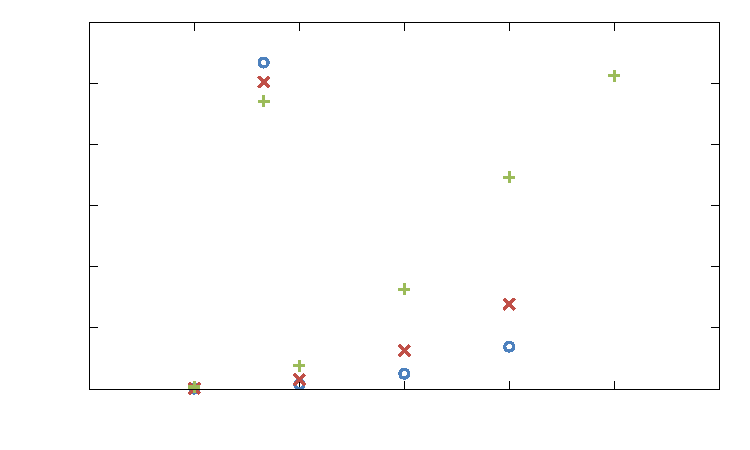
\includegraphics{GRAPH_Mag_vs_galaxies_in_time_Euclid}}%
    \gplfronttext
  \end{picture}%
\endgroup

				}\endgroup
		\caption{Number of galaxies expected for different magnitudes, given set overall observing time for the Euclid Space Telescope.\label{fig:galaxies_expected_EST}}
	\end{figure}

	For increasing magnitudes, the total number of objects given a total observing time was found to increase within the range \numrange{27}{31}. A survey of \SI{0.1e6}{\second} for each filter yielded best results at a magnitude of 29.5. Around 70 galaxies between a redshift of 8.5 and 10 would be expected. However this would involve one pointing of the telescope, which would lead to a large uncertainty on the number due to cosmic variance.
	\begin{figure}[htbp]
		\centering
			\begingroup\endlinechar=-1
				\resizebox{0.8\textwidth}{!}{%
					% GNUPLOT: LaTeX picture with Postscript
\begingroup
  \makeatletter
  \providecommand\color[2][]{%
    \GenericError{(gnuplot) \space\space\space\@spaces}{%
      Package color not loaded in conjunction with
      terminal option `colourtext'%
    }{See the gnuplot documentation for explanation.%
    }{Either use 'blacktext' in gnuplot or load the package
      color.sty in LaTeX.}%
    \renewcommand\color[2][]{}%
  }%
  \providecommand\includegraphics[2][]{%
    \GenericError{(gnuplot) \space\space\space\@spaces}{%
      Package graphicx or graphics not loaded%
    }{See the gnuplot documentation for explanation.%
    }{The gnuplot epslatex terminal needs graphicx.sty or graphics.sty.}%
    \renewcommand\includegraphics[2][]{}%
  }%
  \providecommand\rotatebox[2]{#2}%
  \@ifundefined{ifGPcolor}{%
    \newif\ifGPcolor
    \GPcolortrue
  }{}%
  \@ifundefined{ifGPblacktext}{%
    \newif\ifGPblacktext
    \GPblacktexttrue
  }{}%
  % define a \g@addto@macro without @ in the name:
  \let\gplgaddtomacro\g@addto@macro
  % define empty templates for all commands taking text:
  \gdef\gplbacktext{}%
  \gdef\gplfronttext{}%
  \makeatother
  \ifGPblacktext
    % no textcolor at all
    \def\colorrgb#1{}%
    \def\colorgray#1{}%
  \else
    % gray or color?
    \ifGPcolor
      \def\colorrgb#1{\color[rgb]{#1}}%
      \def\colorgray#1{\color[gray]{#1}}%
      \expandafter\def\csname LTw\endcsname{\color{white}}%
      \expandafter\def\csname LTb\endcsname{\color{black}}%
      \expandafter\def\csname LTa\endcsname{\color{black}}%
      \expandafter\def\csname LT0\endcsname{\color[rgb]{1,0,0}}%
      \expandafter\def\csname LT1\endcsname{\color[rgb]{0,1,0}}%
      \expandafter\def\csname LT2\endcsname{\color[rgb]{0,0,1}}%
      \expandafter\def\csname LT3\endcsname{\color[rgb]{1,0,1}}%
      \expandafter\def\csname LT4\endcsname{\color[rgb]{0,1,1}}%
      \expandafter\def\csname LT5\endcsname{\color[rgb]{1,1,0}}%
      \expandafter\def\csname LT6\endcsname{\color[rgb]{0,0,0}}%
      \expandafter\def\csname LT7\endcsname{\color[rgb]{1,0.3,0}}%
      \expandafter\def\csname LT8\endcsname{\color[rgb]{0.5,0.5,0.5}}%
    \else
      % gray
      \def\colorrgb#1{\color{black}}%
      \def\colorgray#1{\color[gray]{#1}}%
      \expandafter\def\csname LTw\endcsname{\color{white}}%
      \expandafter\def\csname LTb\endcsname{\color{black}}%
      \expandafter\def\csname LTa\endcsname{\color{black}}%
      \expandafter\def\csname LT0\endcsname{\color{black}}%
      \expandafter\def\csname LT1\endcsname{\color{black}}%
      \expandafter\def\csname LT2\endcsname{\color{black}}%
      \expandafter\def\csname LT3\endcsname{\color{black}}%
      \expandafter\def\csname LT4\endcsname{\color{black}}%
      \expandafter\def\csname LT5\endcsname{\color{black}}%
      \expandafter\def\csname LT6\endcsname{\color{black}}%
      \expandafter\def\csname LT7\endcsname{\color{black}}%
      \expandafter\def\csname LT8\endcsname{\color{black}}%
    \fi
  \fi
  \setlength{\unitlength}{0.0500bp}%
  \begin{picture}(7200.00,4320.00)%
    \gplgaddtomacro\gplbacktext{%
      \put(747,595){\makebox(0,0)[r]{\strut{}-100}}%
      \put(747,947){\makebox(0,0)[r]{\strut{} 0}}%
      \put(747,1299){\makebox(0,0)[r]{\strut{} 100}}%
      \put(747,1651){\makebox(0,0)[r]{\strut{} 200}}%
      \put(747,2003){\makebox(0,0)[r]{\strut{} 300}}%
      \put(747,2355){\makebox(0,0)[r]{\strut{} 400}}%
      \put(747,2707){\makebox(0,0)[r]{\strut{} 500}}%
      \put(747,3059){\makebox(0,0)[r]{\strut{} 600}}%
      \put(747,3411){\makebox(0,0)[r]{\strut{} 700}}%
      \put(747,3763){\makebox(0,0)[r]{\strut{} 800}}%
      \put(747,4115){\makebox(0,0)[r]{\strut{} 900}}%
      \put(849,409){\makebox(0,0){\strut{} 27.5}}%
      \put(1856,409){\makebox(0,0){\strut{} 28}}%
      \put(2864,409){\makebox(0,0){\strut{} 28.5}}%
      \put(3871,409){\makebox(0,0){\strut{} 29}}%
      \put(4878,409){\makebox(0,0){\strut{} 29.5}}%
      \put(5886,409){\makebox(0,0){\strut{} 30}}%
      \put(6893,409){\makebox(0,0){\strut{} 30.5}}%
      \csname LTb\endcsname%
      \put(144,2355){\rotatebox{-270}{\makebox(0,0){\strut{}Number of Galaxies}}}%
      \csname LTb\endcsname%
      \put(3871,130){\makebox(0,0){\strut{}Magnitude ($M$)}}%
      \put(3871,4022){\makebox(0,0){\strut{}}}%
    }%
    \gplgaddtomacro\gplfronttext{%
      \csname LTb\endcsname%
      \put(2178,3670){\makebox(0,0)[r]{\strut{}\SI{0.1e6}{\second}}}%
      \csname LTb\endcsname%
      \put(2178,3484){\makebox(0,0)[r]{\strut{}\SI{0.2e6}{\second}}}%
      \csname LTb\endcsname%
      \put(2178,3298){\makebox(0,0)[r]{\strut{}\SI{0.5e6}{\second}}}%
    }%
    \gplbacktext
    \put(0,0){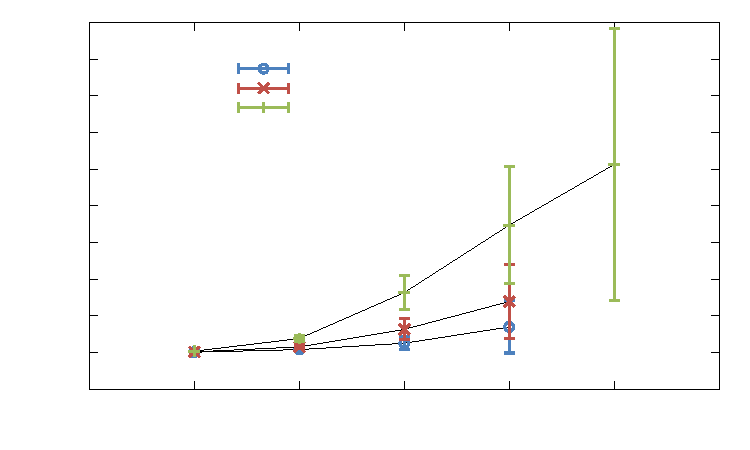
\includegraphics{GRAPH_Mag_vs_galaxies_in_time_Euclid_errors}}%
    \gplfronttext
  \end{picture}%
\endgroup

				}\endgroup
		\caption{Number of galaxies expected for different magnitudes, given set overall observing time for the Euclid Telescope.\label{fig:galaxies_expected_Euclid}}
	\end{figure}

	The alternative option was to double the survey time to \SI{0.2e6}{\second}, which yielded 63 galaxies at a magnitude of 29.0, and increasing the number of pointings (and survey area) by a factor of five, thus reducing the cosmic variance. For the same time, there was also the option of observing around 140 galaxies down to a magnitude of 29.5, with 2 pointings of the telescope.

	In order to keep time to a minimum, it was decided that the \SI{0.1e6}{\second} option was best, as each galaxy needs to be observed in three filters, and subsequently confirmed by spectroscopy. The multi-band photometry approximately triples the \SI{0.1e6}{\second} to \SI{0.3e6}{\second}. Added to this, overhead times extend the time further as the telescope will need to be read out. As an approximation, this increases the total time taken to do photometry to around \SI{0.6e6}{\second}, or 7\,days continuous viewing. The telescope is assumed to be operational for 18\,hours a day, meaning that the shortest time over which this survey could be done is around ten days, not including spectroscopy.
% subsection using_euclid_for_a_survey_of_edshift_8_54_to_10_1 (end)

% part observations (end)

\newpage
\bibliographystyle{unsrt}
\bibliography{references}
\addcontentsline{toc}{section}{References}
\newpage
\appendix
    \addcontentsline{toc}{section}{Appendix}
    %!TEX root = mainfile.tex

\section{Derivation of Thermal Background} % (fold)
\label{sec:derivation_of_thermal_background}
	Number of incident photons, $N_{\gamma}$, is
	\begin{align}
		N_{\gamma} &= \int_{\nu_1}^{\nu_2} \frac{\epsilon B_\nu(T)}{h_nu}\d{\nu}
	\end{align}
	This integral spans the filter from the red to the blue end.
	\begin{align}
		B_\nu(T) &= \frac{2h\nu^3}{c^2}\frac{1}{\e{\frac{h\nu}{kT}}-1}
	\end{align}
	where $\e{\frac{h\nu}{kT}} \ll 1$. Using the substitution
	\begin{align}
		x = \frac{h\nu}{kT}, \qquad \nu &= \frac{kTx}{h} \\
		\Rightarrow \d{\nu} &= \frac{kT}{h}\d{x}
	\end{align}
	$B_\nu(T)$, then, is
	\begin{align}
		B_\nu(T) &= \frac{2k^3 T^3 x^3}{h^2 c^2} \frac{1}{\e{x}}
	\end{align}
	Thus, the number of photons is given by
	\begin{align}
		N_\gamma &= \frac{2 k^3 T^3\epsilon}{h^2 c^2} \int_{x_1}^{x_2}x^2 \e{-x}\d{x} \\
			&= \frac{2 k^3 T^3\epsilon}{h^2 c^2} \left[ -x^2 \e{-x} + \int \e{-x}\cdot 2x\d{x} \right]_{x_1}^{x_2} \\
			&= \frac{2 k^3 T^3\epsilon}{h^2 c^2} \left[ -x^2 \e{-x} -2x\e{-x} + \int 2\e{-x}\d{x} \right]_{x_1}^{x_2} \\
			&= \frac{2 k^3 T^3\epsilon}{h^2 c^2} \Big[ -\e{-x}\left( x^2 + 2x + 2 \right) \Big]_{x_1}^{x_2}
	\end{align}
	By integrating from the blue end of the filter to the red, we can remove the negative sign to give
	\begin{align}
		N_\gamma &= \frac{2 k^3 T^3\epsilon}{h^2 c^2} \Big[\e{-x}\left( x^2 + 2x + 2 \right) \Big]_{x_1}^{x_2}
	\end{align}
% section derivation_of_thermal_background (end)

    %!TEX root = mainfile.tex

\section{Parameter Fit Data} % (fold)
\label{app:parameter_fit_data}
	\subsection{Faint End Slope Data} % (fold)
	\label{sub:alpha_data}
		\begin{table}[!htbp]
			\begin{center}
			\makebox[\linewidth]{
				\begin{tabular}{L|L|L|c|c|c|L|L|c|c|L}
					Rest $\lambda$ (\AA)	&$z$	&error $z$	&$\alpha$	&pos error $\phi^*$	&neg error $\phi^*$	&upper $z$	&lower $z$	&upper 	&lower& Citation\\
					\hline \hline
					1750	&8	&	&-1.91	&0.32	&0.09	&8	&8	&-2	&-1.59	&\cite{}\\
					1750	&8	&	&-1.67	&0.4	&0.4	&8	&8	&-2.07	&-1.27	&\cite{}\\
					1700	&2.3	&0.4	&-1.73	&0.07	&0.07	&2.7	&1.9	&-1.8	&-1.66	&\cite{}\\
					1700	&3.05	&0.35	&-1.73	&0.13	&0.13	&3.4	&2.7	&-1.86	&-1.6	&\cite{}\\
					1500	&7	&0.5	&-1.72	&0	&0	&7.5	&6.5	&-1.72	&-1.72	&\cite{}\\
					1500	&5	&0.3	&-1.66	&0.06	&0.06	&5.3	&4.7	&-1.72	&-1.6	&\cite{}\\
					1500	&6	&0.3	&-1.71	&0.11	&0.11	&6.3	&5.7	&-1.82	&-1.6	&\cite{}\\
					1600	&3.8	&	&-1.76	&0.05	&0.05	&3.8	&3.8	&-1.81	&-1.71	&\cite{}\\
					1600	&5	&	&-1.69	&0.09	&0.09	&5	&5	&-1.78	&-1.6	&\cite{}\\
					1600	&6.8	&	&-1.895	&0.1045	&0	&6.8	&6.8	&-1.895	&-1.791	&\cite{}\\
					1600	&3.8	&	&-1.73	&0.05	&0.05	&3.8	&3.8	&-1.78	&-1.68	&\cite{}\\
					1600	&5	&	&-1.66	&0.09	&0.09	&5	&5	&-1.75	&-1.57	&\cite{}\\
					1350	&5.9	&	&-1.74	&0.16	&0.16	&5.9	&5.9	&-1.9	&-1.58	&\cite{}\\
					1350	&5.9	&	&-1.77	&0.16	&0.16	&5.9	&5.9	&-1.93	&-1.61	&\cite{}\\
				\end{tabular}
			}
			\end{center}
			\caption{Data describing the evolution of the faint end slope parameter, $\alpha$.\label{tab:alpha_data}}
		\end{table}

	% subsection _alpha_data (end)

	\subsection{Normalisation Data} % (fold)
	\label{sub:phi_data}
		\begin{table}[!htbp]
			\begin{center}
			\makebox[\linewidth]{
				\begin{tabular}{L|L|L|c|c|c|L|L|c|c|L}
					Rest $\lambda$ (\AA)	&$z$	&error $z$	&$\phi^*$	&pos error $\phi^*$	&neg error $\phi^*$	&upper $z$	&lower $z$	&upper 	&lower& Citation\\
					\hline \hline
					1750	&8	&	&5.90E-04	&1.01E-03	&3.70E-04	&8	&8	&1.60E-03	&2.20E-04	&\cite{}\\
					1750	&8	&	&1.50E-03	&2.90E-03	&1.00E-03	&8	&8	&4.40E-03	&5.00E-04	&\cite{}\\
					1700	&2.3	&0.4	&2.75E-03	&5.40E-04	&5.40E-04	&2.7	&1.9	&3.29E-03	&2.21E-03	&\cite{}\\
					1700	&3.0	&0.35	&1.71E-03	&5.30E-04	&5.30E-04	&3.4	&2.7	&2.24E-03	&1.18E-03	&\cite{}\\
					1500	&7	&0.5	&7.00E-04	&0	&0	&7.5	&6.5	&7.00E-04	&7.00E-04	&\cite{}\\
					1500	&5	&0.3	&9.00E-04	&2.00E-04	&2.00E-04	&5.3	&4.7	&1.10E-03	&7.00E-04	&\cite{}\\
					1500	&6	&0.3	&1.80E-03	&0	&0	&6.3	&5.7	&1.80E-03	&1.80E-03	&\cite{}\\
					1600	&3.8	&	&1.10E-03	&2.00E-04	&2.00E-04	&3.8	&3.8	&1.30E-03	&9.00E-04	&\cite{}\\
					1600	&5	&	&9.00E-04	&3.00E-04	&2.00E-04	&5	&5	&1.20E-03	&7.00E-04	&\cite{}\\
					1600	&6.8	&	&8.60E-04	&7.00E-04	&3.90E-04	&6.8	&6.8	&1.56E-03	&4.70E-04	&\cite{}\\
					1600	&3.8	&	&1.30E-03	&2.00E-04	&3.00E-04	&3.8	&3.8	&1.50E-03	&1.00E-03	&\cite{}\\
					1600	&5	&	&1.00E-03	&3.00E-04	&3.00E-04	&5	&5	&1.30E-03	&7.00E-04	&\cite{}\\
					1350	&5.9	&	&1.50E-03	&2.90E-03	&1.00E-03	&5.9	&5.9	&4.40E-03	&5.00E-04	&\cite{}\\
					1350	&5.9	&	&1.40E-03	&6.00E-04	&4.00E-04	&5.9	&5.9	&2.00E-03	&1.00E-03	&\cite{}\\
				\end{tabular}
			}
			\end{center}
			\caption{Data describing the evolution of the Schechter normalisation parameter, $\phi^{*}$.\label{tab:phi_star_data}}
		\end{table}
	% subsection phi_data (end)

	\subsection{Characteristic Magnitude Data} % (fold)
	\label{sub:m_data}
		\begin{table}[!htbp]
			\begin{center}
			\makebox[\linewidth]{
				\begin{tabular}{L|c|c|c|c|c|c|c|c|c}
					Rest $\lambda$ (\AA)	&$z$	&error $z$	&$M^*$	&error $M^*$	&upper $z$	&lower $z$	&upper 	&lower& Citation\\
					\hline \hline
					1750	&8	&	&-20.1	&0.52	&8	&8	&-20.62	&-20.1	&\cite{2009ApJ...692..778R}\\
					1750	&8	&	&-19.54	&0.56	&8	&8	&-20.1	&-19.54	&\cite{2009ApJ...692..778R}\\
					1700	&2.3	&0.4	&-20.7	&0.11	&2.7	&1.9	&-20.81	&-20.7	&\cite{2009ApJ...692..778R}\\
					1700	&3.05	&0.35	&-20.97	&0.14	&3.4	&2.7	&-21.11	&-20.97	&\cite{2009ApJ...692..778R}\\
					1500	&7	&0.5	&-20.11	&	&7.5	&6.5	&-20.11	&-20.11	&\cite{2010MNRAS.403..960M}\\
					1500	&5	&0.3	&-20.73	&0.11	&5.3	&4.7	&-20.84	&-20.73	&\cite{2010MNRAS.403..960M}\\
					1500	&6	&0.3	&-20.04	&0.12	&6.3	&5.7	&-20.16	&-20.04	&\cite{2010MNRAS.403..960M}\\
					1600	&3.8	&	&-21.06	&0.1	&3.8	&3.8	&-21.16	&-21.06	&\cite{2007ApJ...670..928B}\\
					1600	&5	&	&-20.69	&0.13	&5	&5	&-20.82	&-20.69	&\cite{2007ApJ...670..928B}\\
					1600	&6.8	&	&-20.14	&0.26	&6.8	&6.8	&-20.4	&-20.14	&\cite{2011ApJ...737...90B}\\
					1600	&3.8	&	&-20.98	&0.1	&3.8	&3.8	&-21.08	&-20.98	&\cite{2011ApJ...737...90B}\\
					1600	&5	&	&-20.64	&0.13	&5	&5	&-20.77	&-20.64	&\cite{2011ApJ...737...90B}\\
					1350	&5.9	&	&-20.24	&0.19	&5.9	&5.9	&-20.43	&-20.24	&\cite{2011ApJ...737...90B}\\
					1350	&5.9	&	&-20.29	&0.19	&5.9	&5.9	&-20.48	&-20.29	&\cite{2007ApJ...670..928B}
				\end{tabular}
			}
			\end{center}
			\caption{Data describing the evolution of the charachteristic magnitude parameter, $M^{*}$.\label{tab:m_star_data}}
		\end{table}
	% subsection m_data (end)
% section paramter_fit_data (end)


\end{document}

